\documentclass{report}
%\usepackage[utopia]{mathdesign}
%\usepackage{amsmath, amsthm}

\usepackage[top=2.5cm, bottom=2.5cm, left=2cm, right=2cm]{geometry}


\usepackage{amsmath,amsfonts,amsthm,amssymb,mathtools}
\usepackage{nicefrac, xfrac}
%\usepackage[varbb]{newpxmath}
%\usepackage[osf,largesc,theoremfont]{newpxtext}
%\usepackage{coelacanth}
%\usepackage{beraserif} % Bitstream Vera Serif font
%\usepackage{berasans} % Bitstream Vera Sans font
%\usepackage{beramono} % Bitstream Vera Sans Mono font
%\usepackage{berasans}
%\usepackage{libertine}
%\usepackage{mathpazo}
%\usepackage{palatino}
%\usepackage{crimson}

% NEW ------- For pointilles lines
\usepackage{multido}
\usepackage{lipsum}

%% Choose one of the following (if not choosing the  
%% default, viz., Computer Modern, font family):
%\usepackage{lmodern}
\usepackage{bold-extra}
%%
%\usepackage{mathpazo}
% \usepackage{newpxmath}
%\usepackage{kpfonts} % Very good
%%
%\usepackage{mathptmx} %Very good
%\usepackage{stix} 
%\usepackage{txfonts} %Very good
\usepackage{newtxtext,newtxmath} %Very good
%%
%\usepackage{libertine} \usepackage[libertine]{newtxmath}
%\usepackage{libertine,libertinust1math} % added 2019/11/28
%%
%\usepackage{newpxtext} \usepackage[euler-digits]{eulervm}
%\usepackage{textcomp}
%\usepackage{bm}
\usepackage{contour}
\usepackage{adjustbox}
\usepackage{nicematrix}
\usepackage{booktabs}
\usepackage{tabularx}




\input{/home/cryptopsy/Semesters/LaTeXTemplates/UniversalTeXTemplate/preamble.tex}
%From M275 "Topology" at SJSU
\newcommand{\id}{\mathrm{id}} % Identité
\newcommand{\taking}[1]{\xrightarrow{#1}} % Flèche avec annotation
\newcommand{\inv}{^{-1}} % Inverse

%From M170 "Introduction to Graph Theory" at SJSU
\DeclareMathOperator{\diam}{diam} % Diamètre
\DeclareMathOperator{\ord}{ord} % Ordre
\newcommand{\defeq}{\overset{\mathrm{def}}{=}} % Défini comme égal

%From the USAMO .tex files
\newcommand{\ts}{\textsuperscript} % Exposant
\newcommand{\dg}{^\circ} % Degré
\newcommand{\ii}{\item} % Item

% % From Math 55 and Math 145 at Harvard
% \newenvironment{subproof}[1][Proof]{%
% \begin{proof}[#1] \renewcommand{\qedsymbol}{$\blacksquare$}}%
% {\end{proof}}

\newcommand{\liff}{\leftrightarrow} % Si et seulement si
\newcommand{\lthen}{\rightarrow} % Implique
\newcommand{\opname}{\operatorname} % Opérateur générique
\newcommand{\surjto}{\twoheadrightarrow} % Flèche surjective
\newcommand{\injto}{\hookrightarrow} % Flèche injective
\newcommand{\On}{\mathrm{On}} % Ordinaux
\DeclareMathOperator{\img}{im} % Image
\DeclareMathOperator{\Img}{Im} % Image
\DeclareMathOperator{\coker}{coker} % Cokernel
\DeclareMathOperator{\Coker}{Coker} % Cokernel
\DeclareMathOperator{\Ker}{Ker} % Noyau
\DeclareMathOperator{\rank}{rank} % Rang
\DeclareMathOperator{\Spec}{Spec} % Spectre
\DeclareMathOperator{\Tr}{Tr} % Trace
\DeclareMathOperator{\pr}{pr} % Projection
\DeclareMathOperator{\ext}{ext} % Extension
\DeclareMathOperator{\pred}{pred} % Prédécesseur
\DeclareMathOperator{\dom}{dom} % Domaine
\DeclareMathOperator{\ran}{ran} % Image (range)
\DeclareMathOperator{\Hom}{Hom} % Homomorphisme
\DeclareMathOperator{\Mor}{Mor} % Morphismes
\DeclareMathOperator{\End}{End} % Endomorphisme

\newcommand{\eps}{\epsilon} % Épsilon
\newcommand{\veps}{\varepsilon} % Variance d'épsilon
\newcommand{\ol}{\overline} % Ligne au-dessus
\newcommand{\ul}{\underline} % Ligne en-dessous
\newcommand{\wt}{\widetilde} % Tilde large
\newcommand{\wh}{\widehat} % Chapeau large
\newcommand{\vocab}[1]{\textbf{\color{blue} #1}} % Texte en gras et bleu
\providecommand{\half}{\frac{1}{2}} % Fraction 1/2
\newcommand{\dang}{\measuredangle} % Angle dirigé
\newcommand{\ray}[1]{\overrightarrow{#1}} % Ray
\newcommand{\seg}[1]{\overline{#1}} % Segment
\newcommand{\arc}[1]{\wideparen{#1}} % Arc
\DeclareMathOperator{\cis}{cis} % cis
\DeclareMathOperator*{\lcm}{lcm} % Plus petit commun multiple
\DeclareMathOperator*{\argmin}{arg min} % Argument du minimum
\DeclareMathOperator*{\argmax}{arg max} % Argument du maximum
\newcommand{\cycsum}{\sum_{\mathrm{cyc}}} % Somme cyclique
\newcommand{\symsum}{\sum_{\mathrm{sym}}} % Somme symétrique
\newcommand{\cycprod}{\prod_{\mathrm{cyc}}} % Produit cyclique
\newcommand{\symprod}{\prod_{\mathrm{sym}}} % Produit symétrique
\newcommand{\Qed}{\begin{flushright}\qed\end{flushright}} % QED aligné à droite
\newcommand{\parinn}{\setlength{\parindent}{1cm}} % Indentation de paragraphe à 1 cm
\newcommand{\parinf}{\setlength{\parindent}{0cm}} % Pas d'indentation de paragraphe
% \newcommand{\norm}{\|\cdot\|} % Norme
\newcommand{\inorm}{\norm_{\infty}} % Norme infinie
\newcommand{\opensets}{\{V_{\alpha}\}_{\alpha\in I}} % Ensemble ouvert
\newcommand{\oset}{V_{\alpha}} % Ensemble ouvert V
\newcommand{\opset}[1]{V_{\alpha_{#1}}} % Ensemble ouvert V avec indice
\newcommand{\lub}{\text{lub}} % Plus petite borne supérieure
\newcommand{\del}[2]{\frac{\partial #1}{\partial #2}} % Dérivée partielle
\newcommand{\Del}[3]{\frac{\partial^{#1} #2}{\partial^{#1} #3}} % Dérivée partielle d'ordre élevé
\newcommand{\deld}[2]{\dfrac{\partial #1}{\partial #2}} % Dérivée partielle avec dfrac
\newcommand{\Deld}[3]{\dfrac{\partial^{#1} #2}{\partial^{#1} #3}} % Dérivée partielle d'ordre élevé avec dfrac
\newcommand{\lm}{\lambda} % Lambda
\newcommand{\uin}{\mathbin{\rotatebox[origin=c]{90}{$\in$}}} % Appartient, tourné de 90 degrés
\newcommand{\usubset}{\mathbin{\rotatebox[origin=c]{90}{$\subset$}}} % Sous-ensemble, tourné de 90 degrés
\newcommand{\lt}{\left} % Gauche
\newcommand{\rt}{\right} % Droite
\newcommand{\bs}[1]{\boldsymbol{#1}} % Symbole en gras
\newcommand{\exs}{\exists} % Il existe
\newcommand{\st}{\strut} % Strut
\newcommand{\dps}[1]{\displaystyle{#1}} % Disposition en ligne

\newcommand{\sol}{\setlength{\parindent}{0cm}\textbf{\textit{Solution:}}\setlength{\parindent}{1cm} } % Solution sans indentation initiale puis rétablie
\newcommand{\solve}[1]{\setlength{\parindent}{0cm}\textbf{\textit{Solution: }}\setlength{\parindent}{1cm}#1 \Qed}

\newcommand{\entoure}[1]{\fcolorbox{black}{gray!30}{\texttt{#1}}}

\renewcommand{\ttdefault}{cmtt}
\newcommand{\textttbf}[1]{\contour{yellow!45}{\texttt{#1}}}
\newcommand{\varitem}[3][black]{%
    \item [%
        \colorbox{#2}{\textcolor{#1}{\makebox(5.5,7){#3}}}%
    ]
}
% Allow you to do the non implication (implication barred)
\newcommand{\notimplies}{%
  \mathrel{{\ooalign{\hidewidth$\not\phantom{=}$\hidewidth\cr$\implies$}}}}


\newcommand*{\authorimg}[1]%
    { \raisebox{-1\baselineskip}{\includegraphics[width=\imagesize]{#1}}}
\newlength\imagesize 

\input{/home/cryptopsy/Semesters/LaTeXTemplates/UniversalTeXTemplate/letterfonts.tex}
% lstlistingsEnvs.tex

\usepackage{minted}


\lstset{
  basicstyle=\ttfamily, % Set
  columns=fullflexible,
  keepspaces=true,
  language=Python % You can specify the language if you want syntax highlighting
}

%%%%%%%%%%%%%%%%%%%%%%%%%%%%%%%%%%%%%%%%%%%%%%%%%%%%%%%%%%%%%%%%%%%%%%%%%%%%%%%%%%%%%%%%%%%%%%%%%
%                                 Custom lstlisting Environments
%%%%%%%%%%%%%%%%%%%%%%%%%%%%%%%%%%%%%%%%%%%%%%%%%%%%%%%%%%%%%%%%%%%%%%%%%%%%%%%%%%%%%%%%%%%%%%%%%
% Gruvbox style for Python
\definecolor{Pgruvbox-bg}{HTML}{282828}
\definecolor{Pgruvbox-fg}{HTML}{ebdbb2}
\definecolor{Pgruvbox-red}{HTML}{fb4934}
\definecolor{Pgruvbox-green}{HTML}{b8bb26}
\definecolor{Pgruvbox-yellow}{HTML}{fabd2f}
\definecolor{Pgruvbox-blue}{HTML}{83a598}
\definecolor{Pgruvbox-purple}{HTML}{d3869b}
\definecolor{Pgruvbox-aqua}{HTML}{8ec07c}
\definecolor{BBBlack}{rgb}{0.05, 0.06, 0.09}



% JAVA LSTLISTING STYLE IN Gruvbox Colorscheme
\definecolor{gruvbox-bg}{rgb}{0.282, 0.247, 0.204}
\definecolor{gruvbox-fg1}{rgb}{0.949, 0.898, 0.776}
\definecolor{gruvbox-fg2}{rgb}{0.871, 0.804, 0.671}
\definecolor{gruvbox-red}{rgb}{0.788, 0.255, 0.259}
\definecolor{gruvbox-green}{rgb}{0.518, 0.604, 0.239}
\definecolor{gruvbox-yellow}{rgb}{0.914, 0.808, 0.427}
\definecolor{gruvbox-blue}{rgb}{0.353, 0.510, 0.784}
\definecolor{gruvbox-purple}{rgb}{0.576, 0.412, 0.659}
\definecolor{gruvbox-aqua}{rgb}{0.459, 0.631, 0.737}
\definecolor{gruvbox-gray}{rgb}{0.518, 0.494, 0.471}

\definecolor{lst-bg}{RGB}{45, 45, 45}
\definecolor{lst-fg}{RGB}{220, 220, 204}
\definecolor{lst-keyword}{RGB}{215, 186, 125}
\definecolor{lst-comment}{RGB}{117, 113, 94}
\definecolor{lst-string}{RGB}{163, 190, 140}
\definecolor{lst-number}{RGB}{181, 206, 168}
\definecolor{lst-type}{RGB}{218, 142, 130}

\lstdefinestyle{PythonGruvbox}{
    language=Python,
    identifierstyle=\color{lst-fg},
    basicstyle=\ttfamily\color{Pgruvbox-fg},
    keywordstyle=\color{Pgruvbox-yellow},
    keywordstyle=[2]\color{Pgruvbox-blue},
    stringstyle=\color{Pgruvbox-green},
    commentstyle=\color{Pgruvbox-aqua},
    backgroundcolor=\color{BBBlack},
    rulecolor=\color{BBBlack},
    showstringspaces=false,
    keepspaces=true,
    captionpos=b,
    breaklines=true,
    tabsize=4,
    showspaces=false,
    numbers=left,
    numbersep=5pt,
    numberstyle=\tiny\color{gray},
    showtabs=false,
    columns=fullflexible,
    morekeywords={True,False,None},
    morekeywords=[2]{and,as,assert,break,class,continue,def,del,elif,else,except,exec,
    finally,for,from,global,if,import,in,is,lambda,nonlocal,not,or,pass,print,raise,
    return,try,while,with,yield},
    morecomment=[s]{"""}{"""},
    morecomment=[s]{'''}{'''},
    morecomment=[l]{\#},
    morestring=[b]",
    morestring=[b]',
    literate=
    {0}{{\textcolor{Pgruvbox-purple}{0}}}{1}
    {1}{{\textcolor{Pgruvbox-purple}{1}}}{1}
    {2}{{\textcolor{Pgruvbox-purple}{2}}}{1}
    {3}{{\textcolor{Pgruvbox-purple}{3}}}{1}
    {4}{{\textcolor{Pgruvbox-purple}{4}}}{1}
    {5}{{\textcolor{Pgruvbox-purple}{5}}}{1}
    {6}{{\textcolor{Pgruvbox-purple}{6}}}{1}
    {7}{{\textcolor{Pgruvbox-purple}{7}}}{1}
    {8}{{\textcolor{Pgruvbox-purple}{8}}}{1}
    {9}{{\textcolor{Pgruvbox-purple}{9}}}{1}
}

% Gruvbox style for Java
\definecolor{gruvbox-bg}{rgb}{0.282, 0.247, 0.204}
\definecolor{gruvbox-fg1}{rgb}{0.949, 0.898, 0.776}
\definecolor{gruvbox-fg2}{rgb}{0.871, 0.804, 0.671}
\definecolor{gruvbox-red}{rgb}{0.788, 0.255, 0.259}
\definecolor{gruvbox-green}{rgb}{0.518, 0.604, 0.239}
\definecolor{gruvbox-yellow}{rgb}{0.914, 0.808, 0.427}
\definecolor{gruvbox-blue}{rgb}{0.353, 0.510, 0.784}
\definecolor{gruvbox-purple}{rgb}{0.576, 0.412, 0.659}
\definecolor{gruvbox-aqua}{rgb}{0.459, 0.631, 0.737}
\definecolor{gruvbox-gray}{rgb}{0.518, 0.494, 0.471}

\lstdefinestyle{JavaGruvbox}{
    language=Java,
    basicstyle=\ttfamily\color{Pgruvbox-fg},
    keywordstyle=\color{Pgruvbox-yellow},
    keywordstyle=[2]\color{lst-type},
    commentstyle=\itshape\color{lst-comment},
    stringstyle=\color{lst-string},
    numberstyle=\color{lst-number},
    backgroundcolor=\color{BBBlack},
    rulecolor=\color{gruvbox-aqua},
    showstringspaces=false,
    keepspaces=true,
    captionpos=b,
    breaklines=true,
    tabsize=4,
    showspaces=false,
    showtabs=false,
    columns=fullflexible,
    morekeywords={var},
    morekeywords=[2]{boolean, byte, char, double, float, int, long, short, void},
    morecomment=[s]{/}{/},
    morecomment=[l]{//},
    morestring=[b]",
    morestring=[b]',
    numbers=left,
    numbersep=5pt,
    numberstyle=\tiny\color{gray},
}

% Dracula style for Java
\definecolor{draculawhite-background}{RGB}{237, 239, 252}
\definecolor{draculawhite-comment}{RGB}{98, 114, 164}
\definecolor{draculawhite-keyword}{RGB}{189, 147, 249}
\definecolor{draculawhite-string}{RGB}{152, 195, 121}
\definecolor{draculawhite-number}{RGB}{249, 189, 89}
\definecolor{draculawhite-operator}{RGB}{248, 248, 242}

\lstdefinestyle{JavaDraculaWhite}{
    language=Java,
    backgroundcolor=\color{draculawhite-background},
    commentstyle=\itshape\color{draculawhite-comment},
    keywordstyle=\color{draculawhite-keyword},
    stringstyle=\color{draculawhite-string},
    basicstyle=\ttfamily\footnotesize\color{black},
    identifierstyle=\color{black},
    keywordstyle=\color{draculawhite-keyword}\bfseries,
    morecomment=[s][\color{draculawhite-comment}]{/**}{*/},
    showstringspaces=false,
    showspaces=false,
    breaklines=true,
    %frame=single,
    rulecolor=\color{draculawhite-operator},
    tabsize=2,  
    numbers=left,
    numbersep=4pt,
    numberstyle=\ttfamily\tiny\color{gray}
}

% Dracula style for Python
\definecolor{draculawhite-bg}{HTML}{FAFAFA}
\definecolor{draculawhite-fg}{HTML}{282A36}
\definecolor{pdraculawhite-keyword}{HTML}{BD93F9}
\definecolor{pdraculawhite-comment}{HTML}{6272A4}
\definecolor{draculawhite-number}{HTML}{FF79C6}

\lstdefinestyle{PythonDraculaWhite}{
    language=Python,
    basicstyle=\ttfamily\small\color{draculawhite-fg},
    backgroundcolor=\color{draculawhite-background},
    keywordstyle=\color{orange}\bfseries,
    stringstyle=\color{draculawhite-string},
    commentstyle=\color{pdraculawhite-comment}\itshape,
    numberstyle=\color{draculawhite-number},
    showstringspaces=false,
    showspaces=false,
    breaklines=true,
    frame=single,
    rulecolor=\color{draculawhite-operator}, 
    tabsize=4,
    morekeywords={as,with,1,2,3,4, 5,6,7,8,9,True,False},
    numbers=left,
    numbersep=5pt,
    numberstyle=\small\bfseries\ttfamily\color{htmlcomment},
}

% Dracula Dark style for HTML
\definecolor{htmltag}{HTML}{ff79c6}
\definecolor{htmlattr}{HTML}{f1fa8c}
\definecolor{htmlvalue}{HTML}{bd93f9}
\definecolor{htmlcomment}{HTML}{6272a4}
\definecolor{htmltext}{HTML}{401E31}
\definecolor{htmlbackground}{HTML}{282a36}
\definecolor{comphtmlbackground}{HTML}{8093FF}

\lstdefinestyle{HTMLDraculaDark}{
    basicstyle=\normalsize\bfseries\ttfamily\color{htmltext},
    commentstyle=\itshape\color{htmlcomment},
    keywordstyle=\bfseries\color{htmltag},
    stringstyle=\color{htmlvalue},
    emph={DOCTYPE,html,head,body,div,span,a,script},
    emphstyle={\color{htmltag}\bfseries},
    sensitive=true,
    showstringspaces=false,
    backgroundcolor=\color{white},
    inputencoding=utf8,
    extendedchars=true,
    language=HTML,
    tabsize=4,
    breaklines=true,
    breakatwhitespace=true,
    numbers=left,
    numbersep=10pt,
    numberstyle=\small\bfseries\ttfamily\color{htmlcomment},
    escapeinside={<@}{@>},
    rulecolor=\color{htmlbackground},
    xleftmargin=10pt,
    frame=none, 
    breaklines=true,
    postbreak=\mbox{\textcolor{gray}{$\hookrightarrow$}\space},
    showlines=false,
    moredelim=[s][\itshape\color{htmlcomment}]{<!--}{-->},
    morekeywords={id,class,type,name,value,placeholder,checked,src,href,alt},
    literate={é}{{\'e}}1 {è}{{\`e}}1 {ê}{{\^e}}1 {ë}{{\"e}}1 {à}{{\`a}}1 {ù}{{\`u}}1 {û}{{\^u}}1 {ç}{{\c{c}}}1 {â}{{\^a}}1 {î}{{\^i}}1 {ï}{{\"i}}1
}


\lstdefinestyle{Haskell}{
  frame=none,
  xleftmargin=2pt,
  stepnumber=1,
  numbers=left,
  numbersep=5pt,
  numberstyle=\ttfamily\tiny\color[gray]{0.3},
  belowcaptionskip=\bigskipamount,
  captionpos=b,
  escapeinside={*'}{'*},
  language=haskell,
  tabsize=2,
  emphstyle={\bf},
  %commentstyle=\it,
  stringstyle=\mdseries\ttfamily,
  showspaces=false,
  keywordstyle=\bfseries\ttfamily,
  columns=flexible,
  basicstyle=\small\ttfamily,
  showstringspaces=false,
  morecomment=[l]\%,
}



\lstdefinestyle{CSSDraculaLight}{
    basicstyle=\bfseries\scriptsize\ttfamily\color{htmltext},
    commentstyle=\color{htmlcomment},
    keywordstyle=\bfseries\color{htmlvalue},
    stringstyle=\color{htmlvalue},
    emph={DOCTYPE,html,head,body,div,span,a,script},
    emphstyle={\color{htmltag}\bfseries},
    sensitive=true,
    showstringspaces=false,
    backgroundcolor=\color{white},
    inputencoding=utf8,
    extendedchars=true, % Support extended characters
    frame=none, 
    %frame=tb,
    tabsize=4,
    breaklines=true,
    breakatwhitespace=true,
    numbers=left,
    numbersep=10pt,
    numberstyle=\small\bfseries\ttfamily\color{htmlcomment},
    escapeinside={<@}{@>},
    rulecolor=\color{htmlbackground},
    xleftmargin=20pt,
    % Add a vertical line for opening and closing tags
    %frame=lines,
    framesep=2pt,
    framexleftmargin=4pt,
    % Add a vertical line for closing tags that go through multiple lines
    breaklines=true,
    postbreak=\mbox{\textcolor{gray}{$\hookrightarrow$}\space},
    showlines=true,
    % Add a rule to apply commentstyle to keywords inside comments
    moredelim=[s][\color{htmlcomment}]{/*}{*/},
    literate={é}{{\'e}}1
             {è}{{\`e}}1
             {ê}{{\^e}}1
             {ë}{{\"e}}1
             {à}{{\`a}}1
             {ù}{{\`u}}1
             {û}{{\^u}}1
             {ç}{{\c{c}}}1
             {â}{{\^a}}1
             {î}{{\^i}}1
             {ï}{{\"i}}1,
    morekeywords={color, background, background-color, font-size, font-weight, border, border-radius, padding, margin, display, position, top, right, bottom, left, flex, grid, width, height, min-width, max-width, min-height, max-height, transition, transform, animation, keyframes, content, z-index,id,class,type,name,value,placeholder,checked,src,href,alt},
    morestring=[s][\color{htmltag}]{:}{;},
}


\usetikzlibrary{decorations.pathreplacing}


\def\blankpage{%
      \clearpage%
      \thispagestyle{empty}%
      \addtocounter{page}{-1}%
      \null%
      \clearpage}





\title{\huge{IFT-1575}\\\Huge{Modèles de recherche opérationnelle}\\\vspace{2em} Introduction}
\author{\huge{Franz Girardin}}
\date{\today}



% NEW for point lines
\newcommand{\Pointilles}[1]{%
  \par\nobreak
  \noindent\rule{0pt}{1.5\baselineskip}% Provides a larger gap between the preceding paragraph and the dots
  \multido{}{#1}{\noindent\makebox[\linewidth]{\dotfill}\endgraf}% ... dotted lines ...
  \bigskip% Gap between dots and next paragraph
}
% Define a new command for dotted lines that works in align
\newcommand{\PointillesAlign}{%
  \multido{}{1}{\makebox[\linewidth]{\dotfill}}
}

   

\begin{document}
\setlength{\columnsep}{1cm}
\pagestyle{empty}
\begin{tikzpicture}[remember picture,overlay]

% Fill the background with BlueViolet color
\fill[myb] (current page.south west) rectangle (current page.north east);

% Hexagon pattern on the left
\foreach \i in {2.5,3,...,22} {
    \node[
        rounded corners,
        myb!90,
        draw,
        regular polygon,
        regular polygon sides=6,
        minimum size=\i cm,
        ultra thick
    ] at ($(current page.west)+(2.5,-5)$) {};
}

% Central hexagon with the year
\node[
    rounded corners,
    fill=myb!95,
    text=myb!5,
    regular polygon,
    regular polygon sides=6,
    minimum size=2.5cm,
    inner sep=0,
    ultra thick
] at ($(current page.west)+(2.5,-5)$) {\LARGE \bfseries };

% Hexagon pattern at the top left
\foreach \i in {0.5,1,...,22} {
    \node[
        rounded corners,
        myb!90,
        draw,
        regular polygon,
        regular polygon sides=6,
        minimum size=\i cm,
        ultra thick
    ] at ($(current page.north west)+(2.5,0)$) {};
}

% Hexagon pattern at the top right
\foreach \i in {0.5,1,...,22} {
    \node[
        rounded corners,
        myb!98,
        draw,
        regular polygon,
        regular polygon sides=6,
        minimum size=\i cm,
        ultra thick
    ] at ($(current page.north east)+(0,-9.5)$) {};
}

% Hexagon pattern at the bottom right
\foreach \i in {12} {
    \node[
        fill=myb,
        rounded corners,
        draw=myb,
        regular polygon,
        regular polygon sides=6,
        minimum size=\i cm,
        ultra thick
    ] at ($(current page.south east)+(-0.2,-0.45)$) {};
}

\foreach \i in {21,20,...,6} {
    \node[
        myb!95,
        rounded corners,
        draw,
        regular polygon,
        regular polygon sides=6,
        minimum size=\i cm,
        ultra thick
    ] at ($(current page.south east)+(-0.2,-0.45)$) {};
}

% Title of the report
\node[
    left,
    myb!5,
    minimum width=0.625\paperwidth,
    minimum height=3cm,
    rounded corners
] at ($(current page.north east)+(0,-9.5)$) {\fontsize{25}{30}\selectfont \bfseries IFT-1575};

% Subtitle of the report
\node[
    left,
    myb!10,
    minimum width=0.625\paperwidth,
    minimum height=2cm,
    rounded corners
] at ($(current page.north east)+(0,-11)$) {\huge \text{Modèle de Recherche Opérationelle}};

% Author name
\node[
    left,
    myb!5,
    minimum width=0.625\paperwidth,
    minimum height=2cm,
    rounded corners
] at ($(current page.north east)+(0,-13)$) {\Large \textsc{Franz Girardin}};

\end{tikzpicture}
\clearpage
\newpage
\pdfbookmark[section]{\contentsname}{toc}
\tableofcontents
\clearpage
\pagebreak


\setcounter{page}{1}
\pagestyle{plain}

\begin{multicols*}{2}
\chapter{Algorithme du Simplexe}
\section{Forme algébrique de l'algorithme}
\begin{itemize}
    \item[$\blacktriangleright$] \textbf{Forme standard} :
    \begin{align*}
        \text{Minimiser } & z = c_1x_1 + c_2x_2 + \dots + c_nx_n \\
        \text{s.a. } &
        \begin{cases}
            a_{11}x_1 + a_{12}x_2 + \dots + a_{1n}x_n \leq b_1 \\
            \vdots \\
            a_{m1}x_1 + a_{m2}x_2 + \dots + a_{mn}x_n \leq b_m \\
            x_1, x_2, \dots, x_n \geq 0
        \end{cases}
    \end{align*}

    \item[$\blacktriangleright$] \textbf{Introduction des variables d'écart} $s_i$ :
    \[
    a_{i1}x_1 + a_{i2}x_2 + \dots + a_{in}x_n + s_i = b_i, \quad s_i \geq 0
    \]

    \item[$\blacktriangleright$] \textbf{Fonction objectif ajustée} :
    \[
    z + c_1x_1 + c_2x_2 + \dots + c_nx_n = 0
    \]

    \item[$\blacktriangleright$] \textbf{Choix de la variable entrante} :
    \begin{itemize}
        \item[$\rhd$] Sélectionner la variable avec le coefficient \textbf{le plus négatif} dans la fonction objectif.
    \end{itemize}

    \item[$\blacktriangleright$] \textbf{Détermination de la variable sortante} :
    \begin{itemize}
        \item[$\rhd$] Calculer le \textbf{ratio} pour chaque contrainte :
        \[
        \boxed{\text{Ratio} = \dfrac{b_i}{a_{ij}}} \quad \text{avec } a_{ij} > 0
        \]
        \item[$\rhd$] La variable avec le plus petit ratio positif est la \textbf{variable sortante}.
        \item[$\rhd$] Si tous les $a_{ij}$ sont négatifs, on conclue 
            alors que le problème est \textbf{non borné}                        .
    \end{itemize}

    \item[$\blacktriangleright$] \textbf{Pivot} :
    \begin{itemize}
        \item[$\rhd$] Mettre à jour le tableau en pivotant sur le coefficient correspondant.
    \end{itemize}

    \item[$\blacktriangleright$] \textbf{Critère d'optimalité} :
    \begin{itemize}
        \item[$\rhd$] Si tous les coefficients $\overline{c}_j$de la fonction objectif sont tels que 
            $\overline{c}_j \geq 0$, la solution est optimale.
    \end{itemize}

    \item[$\blacktriangleright$] \textbf{Formules importantes} :
    \begin{itemize}
        \item[$\rhd$] \textbf{Mise à jour des coefficients} :
        \begin{align*}
            & \text{Nouvelle ligne pivot} : 
         \\ &\quad \hspace{-2em}\boxed{\text{Ligne pivot} \div \text{Coefficient pivot}} \\
            & \text{Autres lignes} : 
         \\ &\hspace{-4em}\boxed{\text{Ligne} - (\text{Coefficient} \times \text{Nouvelle ligne pivot})}
        \end{align*}
    \end{itemize}

    \item[$\blacktriangleright$] \textbf{Résumé des étapes} :
    \begin{enumerate}
        \item[$\rhd$] Formuler le problème en forme standard.
        \item[$\rhd$] Identifier la variable entrante (coefficient le plus négatif).
        \item[$\rhd$] Trouver la variable sortante (plus petit ratio positif).
        \item[$\rhd$] Effectuer le pivot.
        \item[$\rhd$] Répéter jusqu'à optimalité.
    \end{enumerate}
\end{itemize}

\section{Forme Tabulée de l'algorithme}
\begin{itemize}
    \item[$\blacktriangleright$] \textbf{Construction du Tableau Simplexe} :
    \begin{itemize}
        \item[$\rhd$] Organiser les équations du problème en \textbf{forme standard} dans un tableau.
        \item[$\rhd$] La première colonne contient les \textbf{variables de base} (variables dépendantes).
        \item[$\rhd$] Chaque ligne représente une équation, y compris la fonction objectif négative $(-z)$.
    \end{itemize}
\begin{alignat*}{4}
    &\text{Min} &\quad -8x & - 6y &\\
    &\text{s.a.} \\
    &\phantom{\text{Min}} &\quad 5x & + 3y & 
    + \; \textcolor{myr}{\boldsymbol{u}}& 
    \phantom{+ \; \textcolor{myr}{\boldsymbol{ p}}} 
    \phantom{+ \;\textcolor{myr}{\boldsymbol{ h}}} \leq 30 & 
    \\
    &\phantom{\text{Min}} &\quad 2x & + 3y & 
    \phantom{+\textcolor{myr}{\boldsymbol{ u}}}& + 
    \textcolor{myr}{\boldsymbol{ p}} 
    \phantom{+\;\textcolor{myr}{\boldsymbol{ h}}} 
    \leq 24 & \\
    &\phantom{\text{Min}} &\quad x & + 3y & 
    \phantom{+\textcolor{myr}{\boldsymbol{ u}}}&  
    \phantom{+\;\textcolor{myr}{\boldsymbol{ p}}} 
    +\textcolor{myr}{\boldsymbol{ h}} \leq 18 & \\ 
    \\ 
    \\
                &\phantom{\text{Min}} &\quad x &, \phantom{+3} y,& 
    \textcolor{myr}{\boldsymbol{u}}&,
    \textcolor{myr}{\boldsymbol{ p}}, 
    \textcolor{myr}{\boldsymbol{ h}}
    \phantom{+\textcolor{myr}{\boldsymbol{ p}}} \geq 0 & \\
\end{alignat*}


        \begin{table}[H]
                \begin{center}
                    \renewcommand{\arraystretch}{1.5}
                    \fontfamily{flr}\selectfont
                    \footnotesize
                        \begin{tabular}{|l|l l l l l |l|l|}
                        \arrayrulecolor{myb}
                        \hline
                        v.d. & $\phantom{-}x$
                             & $\phantom{-}y$ & $\phantom{-}u$ & $\phantom{-}p$ & $\phantom{-}h$ & $-z$ & t.d 
                        \\
                        \hline
                        \arrayrulecolor{black}
                        $\phantom{-}\textcolor{myr}{\boldsymbol{u}}$     
                                & $\phantom{-}5$
                                & $\phantom{-}3$
                                & 1
                                & 
                                & &  &  30
                        \\
                        $\phantom{-}\textcolor{myr}{\boldsymbol{p}}$     
                               & $\phantom{-}2$
                               & $\phantom{-}3$
                               & & 1
                               & & & 24 
                        \\
                        $\phantom{-}\textcolor{myr}{\boldsymbol{h}}$     
                               & $\phantom{-}1$
                               & $\phantom{-}3$ 
                               &  & 
                               &  1
                               & & 18 
                        \\ 
                        \hline
                        $-z$ 
                                & $-8$
                                & $-6$
                                & 
                                & 
                                & 
                                & 1 & 0 
                        \\
                        \hline 



                        \end{tabular}
                \end{center}
                \caption{État initial de la \textbf{forme  standard}}
        \end{table}       
    
    \item[$\blacktriangleright$] \textbf{Choix de la Variable Entrante} :
    \begin{itemize}
        \item[$\rhd$] Sélectionner la variable avec le coefficient le plus négatif dans la ligne $(-z)$.
        \item[$\rhd$] Cette variable améliorera le plus la valeur de l'objectif.
    \end{itemize}
        \begin{table}[H]
                \begin{center}
                    \renewcommand{\arraystretch}{1.5}
                    \fontfamily{flr}\selectfont
                    \footnotesize
                        \begin{tabular}{|l|l l l l l |l|l|}
                        \arrayrulecolor{myb}
                        \hline
                        v.d. & \;\textcolor{myb}{\circled{$x$}} 
                             & $\phantom{-}y$ & $\phantom{-}u$ & $\phantom{-}p$ & $\phantom{-}h$ & $-z$ & t.d 
                        \\
                        \hline
                        \arrayrulecolor{black}
                        $\phantom{-}\textcolor{myr}{\boldsymbol{u}  } 
                        $     & $\phantom{-}5$
                                & $\phantom{-}3$
                                & 1
                                & 
                                & &  &  30
                        \\
                        $\phantom{-}\textcolor{myr}{\boldsymbol{p}  } $     
                               & $\phantom{-}2$
                               & $\phantom{-}3$
                               & & 1
                               & & & 24 
                        \\
                        $\phantom{-}\textcolor{myr}{\boldsymbol{h}  } $     
                               & $\phantom{-}1$
                               & $\phantom{-}3$ 
                               &  & 
                               &  1
                               & & 18 
                        \\ 
                        \hline
                        $-z$ 
                               & \cellcolor{myb!40}$-8$
                                & $-6$
                                & 
                                & 
                                & 
                                & 1 & 0 
                        \\
                        \hline 



                        \end{tabular}
                \end{center}
        \caption{Variable d'entrée choisie}
        \end{table}
    
    \item[$\blacktriangleright$] \textbf{Détermination de la Variable Sortante} :
    \begin{itemize}
        \item[$\rhd$] Calculer les \textbf{ratios} pour chaque variable de base :
        \[
        \boxed{\text{Ratio} = \dfrac{\text{Terme de droite}}{\text{Coefficient de la variable entrante}}}
        \]
        \item[$\rhd$] Ignorer les coefficients négatifs ou nuls de la variable entrante.
        \item[$\rhd$] La variable avec le plus petit ratio positif est la \textbf{variable sortante}.
    \end{itemize}
\noindent
\textbf{Exemple} 
\begin{align*}
    &\text{lim}(\textcolor{myr}{\boldsymbol{u}} ) = 
    \text{t.d.}(\textcolor{myr}{\boldsymbol{u}}) \div 
    x(\textcolor{myr}{\boldsymbol{u}}) = 30 \div 5 = \textcolor{myr}{\boldsymbol{6}}
    \\
    &\text{lim}(\textcolor{myr}{\boldsymbol{p}} ) = 
\text{t.d.}(\textcolor{myr}{\boldsymbol{p}}) \div 
    x(\textcolor{myr}{\boldsymbol{p}}) = 24 \div 2 = 12 
    \\
    &\text{lim}(\textcolor{myr}{\boldsymbol{h}}) = 
\text{t.d.}(\textcolor{myr}{\boldsymbol{h}}) \div 
    x(\textcolor{myr}{\boldsymbol{h}}) = 18 \div 1 = 12 
\end{align*}

    
    \item[$\blacktriangleright$] \textbf{Pivot} :
    \begin{itemize}
        \item[$\rhd$] Identifier le \textbf{coefficient pivot} à l'intersection de la colonne de la variable entrante et de la ligne de la variable sortante.
        \item[$\rhd$] Diviser la ligne pivot par le coefficient pivot pour obtenir un 1.
        \item[$\rhd$] Utiliser des opérations sur les lignes pour annuler les autres coefficients dans la colonne de la variable entrante.
    \end{itemize}


        \begin{table}[H]
                \begin{center}
                    \renewcommand{\arraystretch}{1.5}
                    \fontfamily{flr}\selectfont
                    \footnotesize
                        \begin{tabular}{|l|l l l l l |l|l|}
                        \arrayrulecolor{myb}
                        \hline
                        v.d. & $\phantom{-}x$
                             & $\phantom{-}y$ & $\phantom{-}u$ & $\phantom{-}p$ & $\phantom{-}h$ & $-z$ & t.d 
                        \\
                        \hline
                        \arrayrulecolor{black}
                        $\phantom{-}\textcolor{myr}{\boldsymbol{u \rightarrow x}} 
                        $     & $\phantom{-}5$ 
                                & $\phantom{-}3$
                                & $\phantom{-}1$
                                & 
                                & &  &  30
                        \\
                        $\phantom{-}p$     
                               & $\phantom{-}2$
                               & $\phantom{-}3$
                               & & 1
                               & & & 24 
                        \\
                        $\phantom{-}h$     
                               & $\phantom{-}1$
                               & $\phantom{-}3$ 
                               &  & 
                               &  1
                               & & 18 
                        \\ 
                        \hline
                        $-z$ 
                               & $-8$
                                & $-6$
                                & 
                                & 
                                & 
                                & 1 & 0 
                        \\
                        \hline 



                        \end{tabular}
                \end{center}
        \caption{État durant le pivot}
        \end{table}

 \begin{table}[H]
                \begin{center}
                    \renewcommand{\arraystretch}{1.5}
                    \fontfamily{flr}\selectfont
                    \footnotesize
                        \begin{tabular}{|l|l l l l l |l|l|}
                        \arrayrulecolor{myb}
                        \hline
                        v.d. & $\phantom{-}x$ 
                             & $\phantom{-}y$ & $\phantom{-}u$ & $\phantom{-}p$ & $\phantom{-}h$ & $-z$ & t.d 
                        \\
                        \hline
                        \arrayrulecolor{black}
                        $\textcolor{myr}{\boldsymbol{u \rightarrow x}  } 
                        $     & \;\textcolor{myb}{\circled{$5$}} 
                                & $\phantom{-}3$
                                & $\phantom{-}1$
                                & 
                                & &  &  30
                        \\
                        $\phantom{-}p$     
                               & $\phantom{-}2$
                               & $\phantom{-}3$
                               & & 1
                               & & & 24 
                        \\
                        $\phantom{-}h$     
                               & $\phantom{-}1$
                               & $\phantom{-}3$ 
                               &  & 
                               &  1
                               & & 18 
                        \\ 
                        \hline
                        $-z$ 
                               & $-8$
                                & $-6$
                                & 
                                & 
                                & 
                                & 1 & 0 
                        \\
                        \hline 



                        \end{tabular}
                \end{center}
        \caption{Coefficient du pivot identifié}
        \end{table}   

\begin{table}[H]
                \begin{center}
                    \renewcommand{\arraystretch}{1.5}
                    \fontfamily{flr}\selectfont
                    \footnotesize
                        \begin{tabular}{|l|l l l l l |l|l|}
                        \arrayrulecolor{myb}
                        \hline
                        v.d. & $\phantom{-}x$
                             & $\phantom{-}y$ & $u$ & $\phantom{-}p$ & $\phantom{-}h$ & $-z$ & t.d 
                        \\
                        \hline
                        \arrayrulecolor{black}
                        \rowcolor{myb!40}
                        $\phantom{-}\textcolor{myb}{\boldsymbol{x}}  
                        $     & $\phantom{-}\textcolor{myb}{\boldsymbol{1}}$ 
                              & $\phantom{-}\textcolor{myb}{\boldsymbol{\nicefrac{3}{5}}}$
                                & $\textcolor{myb}{\boldsymbol{\nicefrac{1}{5}}}$
                                & 
                                & &  &  $\textcolor{myb}{\boldsymbol{\nicefrac{30}{5}}}$
                        \\
                        $\phantom{-}\textcolor{myr}{\boldsymbol{p} } $     
                               & $\phantom{-}2$
                               & $\phantom{-}3$
                               & & 1
                               & & & 24 
                        \\
                        $\phantom{-}\textcolor{myr}{\boldsymbol{h}} $     
                               & $\phantom{-}1$
                               & $\phantom{-}3$ 
                               &  & 
                               &  1
                               & & 18 
                        \\ 
                        \hline
                        $-z$ 
                               & $-8$
                                & $-6$
                                & 
                                & 
                                & 
                                & 1 & 0 
                        \\
                        \hline 



                        \end{tabular}
                \end{center}
        \caption{Division par le cofficient du pivot}
        \end{table}


\begin{table}[H]
                \begin{center}
                    \renewcommand{\arraystretch}{1.5}
                    \fontfamily{flr}\selectfont
                    \footnotesize
                        \begin{tabular}{|l|l l l l l |l|l|}
                        \arrayrulecolor{myb}
                        \hline
                        v.d. & $x$
                             & $y$ & $u$ & $p$ & $h$ & $-z$ & t.d 
                        \\
                        \hline
                        \arrayrulecolor{black}
                        \rowcolor{myb!40}
                        $\phantom{-}\textcolor{myb}{\boldsymbol{x}} 
                        $     & $\phantom{-}\textcolor{myb}{\boldsymbol{1}}$ 
                              & $\phantom{-}\textcolor{myb}{\boldsymbol{\nicefrac{3}{5}}}$
                                & $\phantom{-}\textcolor{myb}{\boldsymbol{\nicefrac{1}{5}}}$
                                & 
                                & &  &  $\textcolor{myb}{\boldsymbol{6}}$
                        \\
                        \rowcolor{myb!40}
                        $\phantom{-}\textcolor{myb}{\boldsymbol{p}} $     
                                & $\phantom{-}\textcolor{myb}{\boldsymbol{0}}$             
                                & $\phantom{-}\textcolor{myb}{\boldsymbol{\nicefrac{9}{5}}}$
                                & $\textcolor{myb}{\boldsymbol{-\nicefrac{2}{5}}}$ & 
                                1 & & & $\textcolor{myb}{\boldsymbol{12}}$

                        \\
                        $\phantom{-}h$     
                               & $\phantom{-}1$
                               & $\phantom{-}3$ 
                               &  & 
                               &  1
                               & & 18 
                        \\ 
                        \hline
                        $-z$ 
                               & $-8$
                                & $-6$
                                & 
                                & 
                                & 
                                & 1 & 0 
                        \\
                        \hline 



                        \end{tabular}
                \end{center}
        \caption{$ligne(p) \; - \; 2 \; \times \; ligne(x)$}
        \end{table}


\begin{table}[H]
                \begin{center}
                    \renewcommand{\arraystretch}{1.5}
                    \fontfamily{flr}\selectfont
                    \footnotesize
                        \begin{tabular}{|l|l l l l l |l|l|}
                        \arrayrulecolor{myb}
                        \hline
                        v.d. & $\phantom{-}x$
                             & $\phantom{-}y$ & $\phantom{-}u$ & $p$ & $h$ & $-z$ & t.d 
                        \\
                        \hline
                        \arrayrulecolor{myb}
                        \rowcolor{myb!40}
                        $\phantom{-}\textcolor{myb}{{\boldsymbol{x}}} 
                        $     & $\phantom{-}\textcolor{myb}{{\boldsymbol{1}}}$ 
                              & $\phantom{-}\textcolor{myb}{{\boldsymbol{\nicefrac{3}{5}}}}$
                                & $\phantom{-}\textcolor{myb}{{\boldsymbol{\nicefrac{1}{5}}}}$
                                & 
                                & &  &  $\textcolor{myb}{{\boldsymbol{6}}}$
                        \\
                        \rowcolor{myb!40}
                        $\phantom{-}\textcolor{myb}{{\boldsymbol{p}  }} $     
                                & $\phantom{-}\textcolor{myb}{{\boldsymbol{0}  }}$  
                                & $\phantom{-}\textcolor{myb}{{\boldsymbol{\nicefrac{9}{5}}  }}$
                               & $\textcolor{myb}{{\boldsymbol{-\nicefrac{2}{5}}}}$ & 1 
                               & & & $\textcolor{myb}{{\boldsymbol{12}}}$

                        \\

                        \rowcolor{myb!40}
                    $\phantom{-}\textcolor{myb}{{\boldsymbol{h}  }} $     
                                & $\phantom{-}\textcolor{myb}{{\boldsymbol{0}}}$  
                                & $\phantom{-}\textcolor{myb}{{\boldsymbol{\nicefrac{12}{5}} }}$
                                & $\textcolor{myb}{{\boldsymbol{-\nicefrac{1}{5}}}}$ &  
                                & 1 & & $\textcolor{myb}{{\boldsymbol{12}}}$
                        \\ 
                        \hline
                        $-z$ 
                               & $-8$
                                & $-6$
                                & 
                                & 
                                & 
                                & 1 & 0 
                        \\
                        \hline 



                        \end{tabular}
                \end{center}
        \caption{$ligne(h) \; - \; 1 \; \times \; ligne(x)$}
        \end{table}

\begin{table}[H]
                \begin{center}
                    \renewcommand{\arraystretch}{1.5}
                    \fontfamily{flr}\selectfont
                    \footnotesize
                        \begin{tabular}{|l|l l l l l |l|l|}
                        \arrayrulecolor{myb}
                        \hline
                        v.d. & $\phantom{-}x$
                             & $\phantom{-}y$ & $\phantom{-}u$ & $p$ & $h$ & $-z$ & t.d 
                        \\
                        \hline
                        \arrayrulecolor{myb}
                        \rowcolor{myb!40}
                        $\phantom{-}\textcolor{myb}{{\boldsymbol{x}}} 
                        $     & $\phantom{-}\textcolor{myb}{{\boldsymbol{1}}}$ 
                              & $\phantom{-}\textcolor{myb}{{\boldsymbol{\nicefrac{3}{5}}}}$
                                & $\phantom{-}\textcolor{myb}{{\boldsymbol{\nicefrac{1}{5}}}}$
                                & 
                                & &  &  $\textcolor{myb}{{\boldsymbol{6}}}$
                        \\
                        \rowcolor{myb!40}
                        $\phantom{-}\textcolor{myb}{{\boldsymbol{p}  }} $     
                                & $\phantom{-}\textcolor{myb}{{\boldsymbol{0}  }}$  
                                & $\phantom{-}\textcolor{myb}{{\boldsymbol{\nicefrac{9}{5}}  }}$
                               & $\textcolor{myb}{{\boldsymbol{-\nicefrac{2}{5}}}}$ & 1 
                               & & & $\textcolor{myb}{{\boldsymbol{12}}}$

                        \\

                        \rowcolor{myb!40}
                    $\phantom{-}\textcolor{myb}{{\boldsymbol{h}  }} $     
                                & $\phantom{-}\textcolor{myb}{{\boldsymbol{0}}}$  
                                & $\phantom{-}\textcolor{myb}{{\boldsymbol{\nicefrac{12}{5}} }}$
                                & $\textcolor{myb}{{\boldsymbol{-\nicefrac{1}{5}}}}$ &  
                                & 1 & & $\textcolor{myb}{{\boldsymbol{12}}}$
                        \\ 
                        \hline
                        \rowcolor{myb!40}
                        $\textcolor{myb}{{\boldsymbol{-z} }}$ 
                                &  $\textcolor{myb}{{\boldsymbol{0}}}$
                                & $\textcolor{myb}{{\boldsymbol{-\nicefrac{6}{5}}}}$
                                & $\phantom{-}\textcolor{myb}{{\boldsymbol{\nicefrac{8}{5}}}}$
                                & 
                                & 
                                & 1 & $\textcolor{myb}{{\boldsymbol{48}}}$ 
                        \\
                        \hline 



                        \end{tabular}
                \end{center}
        \caption{$ligne(-z) \; + \; 8 \; \times \; ligne(x)$}
        \end{table}



        Nous avons complété \textbf{une itération} de l'algorithme.
        On obtien alors la solution suivante :
        \begin{align*}
            \boxed{\left[y, u = 0 \right] \implies x = 6, p = 12, h = 12, z = -48}
        \end{align*}

    \item[$\blacktriangleright$] \textbf{Itération} :
    \begin{itemize}
        \item[$\rhd$] Répéter le processus de sélection des variables entrante et sortante, suivi du pivot, jusqu'à ce que tous les coefficients de $(-z)$ soient positifs ou nuls.
    \end{itemize}

        \subsection{Choix de la variable d'entrée}

\begin{table}[H]
                \begin{center}
                    \renewcommand{\arraystretch}{1.5}
                    \fontfamily{flr}\selectfont
                    \footnotesize
                        \begin{tabular}{|l|l l l l l |l|l|}
                        \arrayrulecolor{myb}
                        \hline
                        v.d. & $x$
                             & \; \textcolor{myb}{\circled{$y$}}  & $\phantom{-}u$ & $\phantom{-}p$ & $h$ & $-z$ & t.d 
                        \\
                        \hline
                        \arrayrulecolor{black}
                        $\textcolor{black}{{x}} 
                        $     & $\textcolor{black}{{1}}$ 
                              & $\phantom{-}\textcolor{black}{{\nicefrac{3}{5}}}$
                                & \phantom{-}$\textcolor{black}{{\nicefrac{1}{5}}}$
                                & 
                                & &  &  $\textcolor{black}{{6}}$
                        \\
                        $\textcolor{black}{{p}} $     
                                & $\textcolor{black}{{0}}$  
                                &\phantom{-} $\textcolor{black}{{\nicefrac{9}{5}}}$
                               & $\textcolor{black}{{-\nicefrac{2}{5}}}$ & 1 
                               & & & $\textcolor{black}{{12}}$

                        \\
                    $\textcolor{black}{{h}} $     
                                & $\textcolor{black}{{0}}$  
                                & $\phantom{-}\textcolor{black}{{\nicefrac{12}{5}}}$
                                & $\textcolor{black}{{-\nicefrac{1}{5}}}$ &  
                                & 1 & & $\textcolor{black}{{12}}$
                        \\ 
                        \hline
                        $\textcolor{black}{{-z}}$ 
                                &  $\textcolor{black}{{0}}$
                                & \cellcolor{myb!40}$\textcolor{black}{{-\nicefrac{6}{5}}}$
                                & $\phantom{-}\textcolor{black}{{\nicefrac{8}{5}}}$
                                & 
                                & 
                                & 1 & $\textcolor{black}{{48}}$ 
                        \\
                        \hline 



                        \end{tabular}
                \end{center}
        \end{table}

La variable d'entrée est donc $x_s = \boldsymbol{\textcolor{myb}{y}}$
\section{Choix de la variable de sortie}
\textbf{Démonstration} 
\begin{align*}
    &\text{lim}(\textcolor{myr}{\boldsymbol{x}}) = 
    \text{t.d.}(\textcolor{myr}{\boldsymbol{x}}) \div 
    y(\textcolor{myr}{\boldsymbol{x}} ) = 6  \div \nicefrac{3}{5} = 10
    \\
    &\text{lim}(\textcolor{myr}{\boldsymbol{p}}) = 
    \text{t.d.}(\textcolor{myr}{\boldsymbol{p}}) \div 
    y(\textcolor{myr}{\boldsymbol{p}}) = 12 \div \nicefrac{9}{5} = \nicefrac{20}{3}
    \\
    &\text{lim}(\textcolor{myr}{\boldsymbol{h}}) = 
    \text{t.d.}(\textcolor{myr}{\boldsymbol{h}}) \div 
    y(\textcolor{myr}{\boldsymbol{h}} ) = 18 \div \nicefrac{12}{5} = \textcolor{myr}{\boldsymbol{5}} 
\end{align*}

    La variable de sortie est donc $x_r = \boldsymbol{\textcolor{myr}{h}}$, puisqu'après 
    $y \leq 5$, $h$ devient négatif, ce qui viole la contrainte de \textbf{non négativité}. 


\begin{table}[H]
                \begin{center}
                    \renewcommand{\arraystretch}{1.5}
                    \fontfamily{flr}\selectfont
                    \footnotesize
                        \begin{tabular}{|l|l l l l l |l|l|}
                        \arrayrulecolor{myb}
                        \hline
                        v.d. & $x$
                             & $\phantom{-}y$ & $\phantom{-}u$ & $p$ & $h$ & $-z$ & t.d 
                        \\
                        \hline
                        \arrayrulecolor{black}
                        $\textcolor{black}{{x}} 
                        $     & $\textcolor{black}{{1}}$ 
                              & $\phantom{-}\textcolor{black}{{\nicefrac{3}{5}}}$
                              & $\phantom{-}\textcolor{black}{{\nicefrac{1}{5}}}$
                                & 
                                & &  &  $\textcolor{black}{{6}}$
                        \\
                        $\textcolor{black}{{p}} $     
                                & $\textcolor{black}{{0}}$  
                                & $\phantom{-}\textcolor{black}{{\nicefrac{9}{5}}}$
                               & $\textcolor{black}{{-\nicefrac{2}{5}}}$ & 1 
                               & & & $\textcolor{black}{{12}}$

                        \\
                    $\textcolor{myr}{{\boldsymbol{h \rightarrow y}  }} $     
                                & $\textcolor{black}{{0}}$  
                                & $\textcolor{myb}{\circled{{\nicefrac{12}{5}}}}$
                                & $\textcolor{black}{{-\nicefrac{1}{5}}}$ &  
                                & 1 & & $\textcolor{black}{{12}}$
                        \\ 
                        \hline
                        $\textcolor{black}{{-z}}$ 
                                &  $\textcolor{black}{{0}}$
                                & $\textcolor{black}{{-\nicefrac{6}{5}}}$
                                & $\phantom{-}\textcolor{black}{{\nicefrac{8}{5}}}$
                                & 
                                & 
                                & 1 & $\textcolor{black}{{48}}$ 
                        \\
                        \hline 
                        \end{tabular}
                \end{center}
                \caption{Coefficient de pivot}
        \end{table}



    Puisque le pivot est $\textcolor{myb}{\boldsymbol{\nicefrac{12}{5}}}$, 
    on divise $ligne(h)$ par cette même valeur pour que $y$ soit variable 
    dépendante à $ligne(h)$. 

    \begin{table}[H]
                    \begin{center}
                        \renewcommand{\arraystretch}{1.5}
                        \fontfamily{flr}\selectfont
                        \footnotesize
                            \begin{tabular}{|l|l l l l l |l|l|}
                            \arrayrulecolor{myb}
                            \hline
                            v.d. & $x$
                                 & $\phantom{-}y$ & $\phantom{-}u$ & $p$ & $h$ & $-z$ & t.d 
                            \\
                            \hline
                            \arrayrulecolor{black}
                            $\textcolor{black}{{x}} 
                            $     & $\textcolor{black}{{1}}$ 
                                  & $\phantom{-}\textcolor{black}{{\nicefrac{3}{5}}}$
                                    & $\phantom{-}\textcolor{black}{{\nicefrac{1}{5}}}$
                                    & 
                                    & &  &  $\textcolor{black}{{6}}$
                            \\
                            $\textcolor{black}{{p}} $     
                                    & $\textcolor{black}{{0}}$  
                                    & $\phantom{-}\textcolor{black}{{\nicefrac{9}{5}}}$
                                   & $\textcolor{black}{{-\nicefrac{2}{5}}}$ & 1 
                                   & & & $\textcolor{black}{{12}}$

                            \\

                        \rowcolor{myb!40}
                        $\textcolor{myb}{{\boldsymbol{y}}} $ 
                                    & $\textcolor{myb}{{\boldsymbol{0}}}$  
                                    & $\phantom{-}\textcolor{myb}{{\boldsymbol{1}  }}$
                                    & $\textcolor{myb}{{\boldsymbol{-\nicefrac{1}{12}}}}$ &  
                                    & $\textcolor{myb}{\boldsymbol{\nicefrac{5}{12}}}$ & & $\textcolor{myb}{\boldsymbol{5}}$
                            \\ 
                            \hline
                            $\textcolor{black}{{-z}}$ 
                                    &  $\textcolor{black}{{0}}$
                                    & $\textcolor{black}{{-\nicefrac{6}{5}}}$
                                    & $\phantom{-}\textcolor{black}{{\nicefrac{8}{5}}}$
                                    & 
                                    & 
                                    & 1 & $\textcolor{black}{{48}}$ 
                            \\
                            \hline 
                            \end{tabular}
                    \end{center}
                    \caption{$ligne(h) \div \nicefrac{12}{5}$
                    devient $ligne(y)$
} 
            \end{table}

            On soustrait maintenant $ligne(y)$ à $ligne(p)$ et $ligne(x)$ 
            de façon à avoir un coefficient de 0 sous $y$. 
    \begin{table}[H]
                        \begin{center}
                            \renewcommand{\arraystretch}{1.5}
                            \fontfamily{flr}\selectfont
                            \footnotesize
                                \begin{tabular}{|l|l l l l l |l|l|}
                                \arrayrulecolor{myb}
                                \hline
                                v.d. & $x$
                                     & $\phantom{-}y$ & $\phantom{-}u$ & $p$ & $\phantom{-}h$ & $-z$ & t.d 
                                \\
                                \hline
                                \arrayrulecolor{black}
                                $\textcolor{black}{{x}} 
                                $     & $\textcolor{black}{{1}}$ 
                                      & $\phantom{-}\textcolor{black}{{\nicefrac{3}{5}}}$
                                        & $\phantom{-}\textcolor{black}{{\nicefrac{1}{5}}}$
                                        & 
                                        & &  &  $\textcolor{black}{{6}}$
                                \\
                                \rowcolor{myb!40}
                            $\textcolor{myb}{\boldsymbol{p}} $     
                                        & $\textcolor{myb}{\boldsymbol{0}}$  
                                        & $\phantom{-}\textcolor{myb}{\boldsymbol{0}}$
                                        & $\textcolor{myb}{{\boldsymbol{-\nicefrac{1}{4}}}}$ 
                                        & $\textcolor{myb}{\boldsymbol{1}}$
                                        & $\textcolor{myb}{\boldsymbol{\nicefrac{-3}{4}}}$      
                                        & & $\textcolor{myb}{\boldsymbol{3}}$

                                \\

                            \rowcolor{myb!40}
                            $\textcolor{myb}{{y}} $ 
                                        & $\textcolor{myb}{{0}}$  
                                        & $\phantom{-}\textcolor{myb}{{1}}$
                                        & $\textcolor{myb}{{-\nicefrac{1}{12}}}$ &  
                                        & $\phantom{-}\textcolor{myb}{\nicefrac{5}{12}}$ & & $\textcolor{myb}{5}$
                                \\ 
                                \hline
                                $\textcolor{black}{{-z}}$ 
                                        &  $\textcolor{black}{{0}}$
                                        & $\textcolor{black}{{-\nicefrac{6}{5}}}$
                                        & $\phantom{-}\textcolor{black}{{\nicefrac{8}{5}}}$
                                        & 
                                        & 
                                        & 1 & $\textcolor{black}{{48}}$ 
                                \\
                                \hline 
                                \end{tabular}
                        \end{center}
                        \caption{$ligne(p) \; -  \; \nicefrac{9}{5} \; ligne(y) $}
                \end{table}


    \begin{table}[H]
                        \begin{center}
                            \renewcommand{\arraystretch}{1.5}
                            \fontfamily{flr}\selectfont
                            \footnotesize
                                \begin{tabular}{|l|l l l l l |l|l|}
                                \arrayrulecolor{myb}
                                \hline
                                v.d. & $x$
                                     & $\phantom{-}y$ & $\phantom{-}u$ & $p$ & $\phantom{-}h$ & $-z$ & t.d 
                                \\
                                \hline
                                \arrayrulecolor{black}
                                \rowcolor{myb!40}
                            $\textcolor{myb}{\boldsymbol{x}} $     
                                        & $\textcolor{myb}{\boldsymbol{1}}$  
                                        & $\phantom{-}\textcolor{myb}{\boldsymbol{0}}$
                                        & $\phantom{-}\textcolor{myb}{{\boldsymbol{\nicefrac{1}{4}}}}$ 
                                        & $\textcolor{myb}{\boldsymbol{0}}$
                                        & $\textcolor{myb}{\boldsymbol{\nicefrac{-1}{4}}}$      
                                        & & $\textcolor{myb}{\boldsymbol{3}}$
                                \\
                                \rowcolor{myb!40}
                            $\textcolor{myb}{p} $     
                                        & $\textcolor{myb}{0}$  
                                        & $\phantom{-}\textcolor{myb}{0}$
                                        & $\textcolor{myb}{{-\nicefrac{1}{4}}}$ 
                                        & $\textcolor{myb}{1}$
                                        & $\textcolor{myb}{\nicefrac{-3}{4}}$      
                                        & & $\textcolor{myb}{3}$

                                \\

                            \rowcolor{myb!40}
                            $\textcolor{myb}{{y}} $ 
                                        & $\textcolor{myb}{{0}}$  
                                        & $\phantom{-}\textcolor{myb}{{1}}$
                                        & $\textcolor{myb}{{-\nicefrac{1}{12}}}$ &  
                                        & $\phantom{-}\textcolor{myb}{\nicefrac{5}{12}}$ & & $\textcolor{myb}{5}$
                                \\ 
                                \hline
                                $\textcolor{black}{{-z}}$ 
                                        &  $\textcolor{black}{{0}}$
                                        & $\textcolor{black}{{-\nicefrac{6}{5}}}$
                                        & $\textcolor{black}{{\nicefrac{8}{5}}}$
                                        & 
                                        & 
                                        & 1 & $\textcolor{black}{{48}}$ 
                                \\
                                \hline 
                                \end{tabular}
                        \end{center}
                        \caption{$ligne(x) \; -  \; \nicefrac{3}{5} \; ligne(h) $}
                \end{table}


    \begin{table}[H]
                            \begin{center}
                                \renewcommand{\arraystretch}{1.5}
                                \fontfamily{flr}\selectfont
                                \footnotesize
                                    \begin{tabular}{|l|l l l l l |l|l|}
                                    \arrayrulecolor{myb}
                                    \hline
                                    v.d. & $x$
                                         & $y$ & $\phantom{-}u$ & $p$ & $\phantom{-}h$ & $-z$ & t.d 
                                    \\
                                    \hline
                                    \arrayrulecolor{black}
                                    \rowcolor{myb!40}
                                $\textcolor{myb}{\boldsymbol{x}} $     
                                            & $\textcolor{myb}{\boldsymbol{1}}$  
                                            & $\textcolor{myb}{\boldsymbol{0}}$
                                            & $\phantom{-}\textcolor{myb}{{\boldsymbol{\nicefrac{1}{4}}}}$ 
                                            & $\textcolor{myb}{\boldsymbol{0}}$
                                            & $\textcolor{myb}{\boldsymbol{\nicefrac{-1}{4}}}$      
                                            & & $\textcolor{myb}{\boldsymbol{3}}$
                                    \\
                                    \rowcolor{myb!40}
                                $\textcolor{myb}{\boldsymbol{p}} $     
                                            & $\textcolor{myb}{\boldsymbol{0}}$  
                                            & $\textcolor{myb}{\boldsymbol{0}}$
                                            & $\textcolor{myb}{{\boldsymbol{-\nicefrac{1}{4}}}}$ 
                                            & $\textcolor{myb}{\boldsymbol{1}}$
                                            & $\textcolor{myb}{\boldsymbol{\nicefrac{-3}{4}}}$      
                                            & & $\textcolor{myb}{\boldsymbol{3}}$

                                    \\
                                \rowcolor{myb!40}
                                $\textcolor{myb}{{\boldsymbol{y}  }} $ 
                                            & $\textcolor{myb}{{\boldsymbol{0}  }}$  
                                            & $\textcolor{myb}{{\boldsymbol{1}  }}$
                                            & $\textcolor{myb}{{\boldsymbol{-\nicefrac{1}{12}}}}$ &  
                                            & $\phantom{-}\textcolor{myb}{\boldsymbol{\nicefrac{5}{12}} }$ & 
                                            & $\textcolor{myb}{\boldsymbol{5}  }$
                                    \\ 
                                    \hline
                                    \rowcolor{myb!40}
                                $\textcolor{myb}{\boldsymbol{-z}} $     
                                            & $\textcolor{myb}{\boldsymbol{0}}$  
                                            & $\textcolor{myb}{\boldsymbol{0}}$
                                            & $\phantom{-}\textcolor{myb}{{\boldsymbol{\nicefrac{3}{2}}}}$ 
                                            & $\textcolor{myb}{\boldsymbol{0}}$
                                            & $\phantom{-}\textcolor{myb}{\boldsymbol{\nicefrac{1}{2}}}$      
                                            & $\textcolor{myb}{\boldsymbol{1}}$
                                            & $\textcolor{myb}{\boldsymbol{54}}$
                                    \\
                                    \hline 
                                    \end{tabular}
                            \end{center}
                            \caption{$ligne(-z) \; -  \; \nicefrac{6}{5} \; ligne(h) $}
                    \end{table}

    Nous avons complété \textbf{une seconde itération} de l'algorithme.         
    Le système est associé à la solution :

    \begin{align*}
        \boxed{\left[u, h = 0 \right] \implies x = 3, p = 3, y = 5, z = -54}
    \end{align*}

    Il n’est pas intéressant d’augmenter ni la valeur de $u$, 
    ni la valeur de $h$ car la valeur de $z$ augmente. 
    Ainsi, nous sommes à l’optimum.

    
    \item[$\blacktriangleright$] \textbf{Solution Optimale} :
    \begin{itemize}
        \item[$\rhd$] Lorsque tous les coefficients de $(-z)$ sont positifs ou nuls, la solution optimale est atteinte.
        \item[$\rhd$] Les valeurs des variables de base se trouvent dans la colonne des termes de droite.
    \end{itemize}
    
    \item[$\blacktriangleright$] \textbf{Nombre de Solutions de Base} :
\hspace{-4em}
    \begin{itemize}
        \item[$\rhd$] Pour un système avec $n$ variables et $m$ équations :
        \[
            \hspace{-2em}\boxed{\text{Nombre de solutions de base} = {n \choose m} = \dfrac{n!}{m!(n-m)!}}
        \]
    \end{itemize}
    
    \item[$\blacktriangleright$] \textbf{Résumé des Étapes} :
    \begin{enumerate}
        \item[$\rhd$] \textbf{Organiser} les équations en tableau.
        \item[$\rhd$] \textbf{Choisir} la variable entrante ($x_s$) avec le coefficient le plus négatif dans $(-z)$.
        \item[$\rhd$] \textbf{Déterminer} la variable sortante ($x_r$) avec le plus petit ratio positif.
        \item[$\rhd$] \textbf{Effectuer} le pivot sur le coefficient pivot.
        \item[$\rhd$] \textbf{Répéter} jusqu'à optimalité.
    \end{enumerate}
\end{itemize}

\section{Résolution Graphique}

\begin{itemize}
    \item[$\blacktriangleright$] \textbf{Méthode de Résolution Graphique} (pour problèmes à deux variables) :
    \begin{enumerate}
        \item[$\rhd$] \textbf{Tracer les contraintes} sur un plan cartésien :
        \begin{itemize}
            \item[$\rhd$] Convertir chaque inégalité en équation pour tracer la droite correspondante.
            \item[$\rhd$] Identifier la zone admissible (région des solutions réalisables) en tenant compte des inégalités.
        \end{itemize}
        \item[$\rhd$] \textbf{Déterminer les sommets} de la zone admissible :
        \begin{itemize}
            \item[$\rhd$] Trouver les points d'intersection des droites (sommets du polygone formé).
        \end{itemize}
        \item[$\rhd$] \textbf{Calculer la valeur de la fonction objectif} en chaque sommet :
        \begin{itemize}
            \item[$\rhd$] Évaluer $z = c_1x + c_2y$ pour chaque couple $(x, y)$.
        \end{itemize}
        \item[$\rhd$] \textbf{Choisir la solution optimale} :
        \begin{itemize}
            \item[$\rhd$] Pour une maximisation, sélectionner le sommet avec la valeur de $z$ la plus élevée.
            \item[$\rhd$] Pour une minimisation, choisir le sommet avec la valeur de $z$ la plus faible.
        \end{itemize}
    \end{enumerate}
\end{itemize}

\begin{center}
\begin{tikzpicture}[scale=0.35]
    % Axe des x et des y
    \draw[->] (-1,0) -- (18,0) node[right] {$x$};
    \draw[->] (0,-1) -- (0,12.5) node[above] {$y$};
    
    % Tracer la droite 5x + 3y = 30 en rouge
    \draw[red, thick] (0,10) -- (6,0) 
     node at (3, 11) {$5x + 3y = 30$};
        
    % Tracer la droite x + 3y = 18
    \draw[myg, thick] (0,18/3) -- (18,0) 
     node at (6.5, 6) {$x + 3y = 18$};



    % Tracer la droite 2x + 3y = 24 en bleu
    \draw[blue, thick] (0,8) -- (12,0) 
    node at (4.5,8.5) {$2x + 3y = 24$};
    
    
    % Hachures pour la région de la solution
    \fill[red!20,opacity=0.6] (0,10) -- (6,0) -- (0,0) -- cycle;
    \fill[blue!20,opacity=0.6] (0,8) -- (12,0) -- (0,0) -- cycle;
    \fill[myg!20,opacity=0.6] (0,18/3) -- (18,0) -- (0,0) -- cycle;


 % Tracer les lignes d'intersection plus épaisses
    \draw[myp!70!blue, ultra thick] (0,6) -- (3,5); % Intersection rouge-bleu
    \draw[myp!70!blue, ultra thick] (3,5) -- (6,0); % Intersection rouge-bleu
    \draw[myp!70!blue, ultra thick] (6,0) -- (0,0); % Intersection rouge-bleu
    \draw[myp!70!blue, ultra thick] (0,0) -- (0,6); % Intersection rouge-bleu

    % Hachures pour la région de solution commune, avec une couleur plus foncée
    \fill[red!50!blue!50!myg!50, opacity=0.8] (0,6) -- (3,5) -- (6,0) -- (0,0) -- cycle;
    
    % Ajouter des labels
\end{tikzpicture}
\end{center}

\subsection{Notes Importantes}
\begin{itemize}
    \item[$\blacktriangleright$] \textbf{Dans un problème à deux variables}, la zone admissible est un polygone convexe sur le plan $xy$, et la solution optimale se trouve toujours à l'un des sommets de ce polygone.

    \item[$\blacktriangleright$] \textbf{Vérification de la Faisabilité} :
    \begin{itemize}
        \item[$\rhd$] S'assurer que les points trouvés respectent toutes les contraintes.
    \end{itemize}

    \item[$\blacktriangleright$] \textbf{Cas Particuliers} :
    \begin{itemize}
        \item[$\rhd$] \textbf{Solutions Multiples} : Si la fonction objectif est parallèle à une contrainte bordant la région admissible.
        \item[$\rhd$] \textbf{Région Non Bornée} : Si la région admissible n'est pas limitée, la solution optimale peut être non bornée.
    \end{itemize}
\end{itemize}

\end{multicols*}
\begin{table}[H]
    \centering
    \renewcommand{\arraystretch}{1.5}
    \fontfamily{flr}\selectfont
    \footnotesize
    \resizebox{1\linewidth}{!}{
    \begin{tabular}{|l|*{12}{c}|c|c|}
    \arrayrulecolor{myb}\hline
    v.d. & $x_1$ & $x_2$ & $\cdots$ & $x_r$ & $\cdots$ & $x_m$ &
    $x_{m+1}$ & $\cdots$ & $x_s$ & $\cdots$ & $x_n$ & $-z$ & & t.d. \\
    \hline\arrayrulecolor{black}
    $x_1$ & $1$ & & & & & & $\overline{a}_{1,m+1}$ & $\cdots$ &
    $\overline{a}_{1s}$ & $\cdots$ & $\overline{a}_{1n}$ & & & $\overline{b}_1$ \\
    $x_2$ & & $1$ & & & & & $\overline{a}_{2,m+1}$ & $\cdots$ &
    $\overline{a}_{2s}$ & $\cdots$ & $\overline{a}_{2n}$ & & & $\overline{b}_2$ \\
    $\vdots$ & & & $\ddots$ & & & & & $\ddots$ & & $\ddots$ & & & & $\vdots$ \\
    $x_r$ & & & & $1$ & & & $\overline{a}_{r,m+1}$ & $\cdots$ &
    $\overline{a}_{rs}$ & $\cdots$ & $\overline{a}_{rn}$ & & & $\overline{b}_r$ \\
    $\vdots$ & & & & & $\ddots$ & & $\ddots$ & $\ddots$ & & $\ddots$ &
    $\overline{a}_{1n}$ & & & $\vdots$ \\
    $x_m$ & & & & & & $1$ & $\overline{a}_{m,m+1}$ & $\cdots$ &
    $\overline{a}_{ms}$ & $\cdots$ & $\overline{a}_{mn}$ & & & $\overline{b}_m$ \\
    \hline
    $-z$ & & & & & & & $\overline{c}_{m+1}$ & $\cdots$ &
    $\overline{c}_{s}$ & $\cdots$ & $\overline{c}_{n}$ & $1$ & & $\overline{z}$ \\
    \hline
    \end{tabular}}
\end{table}

% La solution associée est :
% \begin{align*}
%     &x_1 = \overline{b}_1,\quad x_2 = \overline{b}_2,\quad \dots,\quad
%     x_m = \overline{b}_m, \\
%     &x_{m+1} = x_{m+2} = \dots = x_n = 0,\quad z = \overline{z}
% \end{align*}
\begin{multicols*}{2}
\section{Forme Générale de l'Algorithme}

    \begin{itemize}
        \item[$\blacktriangleright$] \textbf{Notations} :
            \begin{itemize}
                \item[$\rhd$] \( x_j \) : Variables de décision, \( j = 1, 2, \dots, n \).
                \item[$\rhd$] \( c_j \) : Coefficients dans la fonction objectif.
                \item[$\rhd$] \( a_{ij} \) : Coefficients des contraintes, \( i = 1, 2, \dots, m \).
                \item[$\rhd$] \( b_i \) : Termes de droite des contraintes.
                \item[$\rhd$] \( x_s \) : Variable d'entrée
                \item[$\rhd$] \( x_r \) : Variable de sortie
            \end{itemize}


        \item[$\blacktriangleright$] \textbf{Forme Standard} :
        \[%
            \begin{aligned}
            &\text{Minimiser } & z = \sum_{j=1}^{n} c_j x_j \\
            &\text{sous contraintes } & \sum_{j=1}^{n} a_{ij} x_j = b_i, \quad i = 1, 2, \dots, m \\
            & & x_j \geq 0, \quad j = 1, 2, \dots, n
            \end{aligned}
        \]%

        \item[$\blacktriangleright$] \textbf{Tableau Simplexe Général} :
            \begin{itemize}
                \item[$\rhd$] Les variables de base \( x_i \) forment une base identité.
                \item[$\rhd$] Les variables non de base sont initialement fixées à zéro.
            \end{itemize}

        \item[$\blacktriangleright$] \textbf{Choix de la Variable Entrante} :
            \begin{itemize}
                \item[$\rhd$] Si tous les coefficients réduits \( \overline{c}_j \geq 0 \), la solution est optimale.
                \item[$\rhd$] Sinon, choisir \( x_s \) tel que :
                \[%
                \boxed{\overline{c}_s = \min \{ c_j \mid j = 1, 2, \dots, n \}}
                \]%
            \end{itemize}

        \item[$\blacktriangleright$] \textbf{Détermination de la Variable Sortante} :
            \begin{itemize}
                \item[$\rhd$] Calculer les ratios pour \( \overline{a}_{is} > 0 \) :
                \[%
                \boxed{\text{Ratio} = \dfrac{\overline{b}_i}{\overline{a}_{is}}}
                \]%
                \item[$\rhd$] La variable sortante \( x_r \) correspond au plus petit ratio positif.
                \item[$\rhd$] Si \( \overline{a}_{is} \leq 0 \) pour tout \( i \), le problème est non borné.
            \end{itemize}

        \item[$\blacktriangleright$] \textbf{Pivot et Mise à Jour du Tableau} :
        \begin{itemize}
            \item[$\rhd$] \textbf{Ligne Pivot} (\( r \)) :
            \[
            \boxed{\text{Nouvelle ligne } r = \dfrac{\text{Ancienne ligne } r}{\overline{a}_{rs}}}
            \]
            \item[$\rhd$] \textbf{Autres Lignes} (\( i \neq r \)) :
            \[
                \hspace{-4em}\boxed{\text{Nouvelle ligne } i = \text{Ancienne ligne } i - \overline{a}_{is} \times \text{Nouvelle ligne } r}
            \]
            \item[$\rhd$] \textbf{Fonction Objectif} :
            \[
                \boxed{\overline{\tilde{c}}_j = \overline{c}_j - \overline{c}_s \times \overline{a}_{rj}}
            \]
            \[
                \boxed{\overline{\tilde{z}} = \overline{z} + \overline{c}_s \times \overline{b}_r}
            \]
        \end{itemize}

    \item[$\blacktriangleright$] \textbf{Résumé des Étapes de l'Algorithme} :
    \begin{enumerate}
        \item[$\rhd$] \textbf{Initialisation} : Formuler le problème en forme standard et construire le tableau initial.
        \item[$\rhd$] \textbf{Itération} :
        \begin{enumerate}
            \item[$\rhd$] Choisir la variable entrante \( x_s \) avec le \( \overline{c}_s \) le plus négatif.
            \item[$\rhd$] Déterminer la variable sortante \( x_r \) en calculant les ratios.
            \item[$\rhd$] Effectuer le pivot pour mettre à jour le tableau.
        \end{enumerate}
        \item[$\rhd$] \textbf{Vérification d'Optimalité} :
        \begin{itemize}
            \item[$\rhd$] Si tous les \( \overline{c}_j \geq 0 \), la solution optimale est atteinte.
            \item[$\rhd$] Sinon, répéter l'itération.
        \end{itemize}
    \end{enumerate}

    \item[$\blacktriangleright$] \textbf{Formules Clés} :
    \begin{itemize}
        \item[$\rhd$] \textbf{Mise à Jour des Coefficients} :
        \[
            \boxed{\overline{\tilde{a}}_{ij} = \overline{a}_{ij} - \overline{a}_{is} \times \overline{a}_{rj}}
        \]
        \item[$\rhd$] \textbf{Mise à Jour des Termes de Droite} :
        \[
            \boxed{\overline{\tilde{b}}_i = \overline{b}_i - \overline{a}_{is} \times \overline{b}_r}
        \]
    \end{itemize}
\end{itemize}
\section{Forme Matricielle de l'Algorithme}

\subsection{Notations Matricielles}

\begin{itemize}
    \item[$\blacktriangleright$] \textbf{Variables de Décision} :
    \[
    \mathbf{x}_{n \times 1} = 
    \begin{bmatrix}
    x_1 \\
    x_2 \\
    \vdots \\
    x_n
    \end{bmatrix}
    \]
    \item[$\blacktriangleright$] \textbf{Coefficients de l'Objectif} :
    \[
    \mathbf{c}_{n \times 1} = 
    \begin{bmatrix}
    c_1 \\
    c_2 \\
    \vdots \\
    c_n
    \end{bmatrix}
    \]
    \item[$\blacktriangleright$] \textbf{Matrice des Contraintes} :
    \[
    \mathbf{A}_{m \times n} = 
    \begin{bmatrix}
    a_{11} & a_{12} & \cdots & a_{1n} \\
    a_{21} & a_{22} & \cdots & a_{2n} \\
    \vdots & \vdots & \ddots & \vdots \\
    a_{m1} & a_{m2} & \cdots & a_{mn}
    \end{bmatrix}
    \]
    \item[$\blacktriangleright$] \textbf{Termes de Droite} :
    \[
    \mathbf{b}_{m \times 1} = 
    \begin{bmatrix}
    b_1 \\
    b_2 \\
    \vdots \\
    b_m
    \end{bmatrix}
    \]
\end{itemize}

\subsection{Formulation Matricielle du Problème}

Le problème de programmation linéaire en forme standard peut être écrit en notation matricielle comme suit :

\begin{align*}
& \text{Minimiser} \quad z = \mathbf{c}^T \mathbf{x} \\
& \text{sous contraintes} \quad \mathbf{A} \mathbf{x} = \mathbf{b} \\
& \quad \quad \quad \quad \quad \mathbf{x} \geq 0
\end{align*}

\subsection{Interprétation}

\begin{itemize}
    \item[$\rhd$] \textbf{Objectif} : \(\mathbf{c}^T \mathbf{x} = \sum_{j=1}^{n} c_j x_j\)
    \item[$\rhd$] \textbf{Contraintes} : Chaque équation \( \sum_{j=1}^{n} a_{ij} x_j = b_i \) est représentée par le produit matriciel \( \mathbf{A} \mathbf{x} = \mathbf{b} \)
    \item[$\rhd$] \textbf{Non-négativité} : \( \mathbf{x} \geq 0 \) signifie que chaque \( x_j \geq 0 \)
\end{itemize}

\subsection{Exemple : Problème du Restaurateur}

Considérons le problème du restaurateur avec les variables \( x \) et \( y \), et les variables d'écart \( u, p, h \).

\begin{align*}
& \text{Minimiser} \quad z = 8x + 6y \\
& \text{sous contraintes} \\
& 5x + 3y + u = 30 \\
& 2x + 3y + p = 24 \\
& x + 3y + h = 18 \\
& x, y, u, p, h \geq 0
\end{align*}

En notation matricielle :

\[
\mathbf{x} = 
\begin{bmatrix}
x \\ y \\ u \\ p \\ h
\end{bmatrix}, \quad
\mathbf{c} = 
\begin{bmatrix}
-8 \\ -6 \\ 0 \\ 0 \\ 0
\end{bmatrix}, \quad
\mathbf{A} = 
\begin{bmatrix}
5 & 3 & 1 & 0 & 0 \\
2 & 3 & 0 & 1 & 0 \\
1 & 3 & 0 & 0 & 1
\end{bmatrix}, \quad
\mathbf{b} = 
\begin{bmatrix}
30 \\ 24 \\ 18
\end{bmatrix}
\]

\subsection{Base et Variables de Base}

\begin{itemize}
    \item[$\blacktriangleright$] Une \textbf{base} \( B \) est une sous-matrice \( m \times m \) non singulière de \( \mathbf{A} \).
    \item[$\blacktriangleright$] Les variables correspondant aux colonnes de \( B \) sont les \textbf{variables de base}.
    \item[$\blacktriangleright$] Les autres variables sont les \textbf{variables hors-base}.
\end{itemize}

\subsubsection{Exemple de Bases}

\[
B_1 = 
\begin{bmatrix}
u & p & h \\
1 & 0 & 0 \\
0 & 1 & 0 \\
0 & 0 & 1
\end{bmatrix}, \quad
B_2 = 
\begin{bmatrix}
x & u & h \\
5 & 1 & 0 \\
2 & 0 & 0 \\
1 & 0 & 1
\end{bmatrix}, \quad
B_3 = 
\begin{bmatrix}
x & p & y \\
5 & 0 & 3 \\
2 & 1 & 3 \\
1 & 0 & 3
\end{bmatrix}
\]

\subsection{Partitionnement des Matrices}

\begin{itemize}
    \item[$\blacktriangleright$] \textbf{Variables} :
    \[
    \mathbf{x} = 
    \begin{bmatrix}
    \mathbf{x}_B \\ \mathbf{x}_R
    \end{bmatrix}
    \]
    où \( \mathbf{x}_B \) sont les variables de base et \( \mathbf{x}_R \) les variables hors-base.
    \item[$\blacktriangleright$] \textbf{Coefficients de l'Objectif} :
    \[
    \mathbf{c} = 
    \begin{bmatrix}
    \mathbf{c}_B \\ \mathbf{c}_R
    \end{bmatrix}
    \]
    \item[$\blacktriangleright$] \textbf{Matrice des Contraintes} :
    \[
    \mathbf{A} = [ B \, : \, R ]
    \]
    où \( B \) est la base et \( R \) le reste de la matrice.
\end{itemize}

\subsection{Formulation Réécrite}

Le problème peut être réécrit comme :

\begin{align*}
& \text{Minimiser} \quad z = \mathbf{c}_B^T \mathbf{x}_B + \mathbf{c}_R^T \mathbf{x}_R \\
& \text{sous contraintes} \quad B \mathbf{x}_B + R \mathbf{x}_R = \mathbf{b} \\
& \mathbf{x}_B \geq 0, \quad \mathbf{x}_R \geq 0
\end{align*}

\subsection{Résolution par le Simplexe en Notation Matricielle}

\begin{enumerate}
    \item \textbf{Expression de \( \mathbf{x}_B \)} :
    \[
    \mathbf{x}_B = B^{-1} \mathbf{b} - B^{-1} R \mathbf{x}_R
    \]
    \item \textbf{Substitution dans l'Objectif} :
    \[
    z = \mathbf{c}_B^T ( B^{-1} \mathbf{b} - B^{-1} R \mathbf{x}_R ) + \mathbf{c}_R^T \mathbf{x}_R
    \]
    \item \textbf{Définition des Multiplicateurs du Simplexe} :
    \[
    \pi^T = \mathbf{c}_B^T B^{-1}
    \]
    \item \textbf{Calcul des Coûts Réduits} :
    \[
    \tilde{\mathbf{c}}_R^T = \mathbf{c}_R^T - \pi^T R
    \]
    \item \textbf{Nouvelle Forme de l'Objectif} :
    \[
    z = \pi^T \mathbf{b} + \tilde{\mathbf{c}}_R^T \mathbf{x}_R
    \]
\end{enumerate}

\subsection{Exemple Numérique}

\begin{itemize}
    \item[$\rhd$] \textbf{Matrice de Base} \( B \) et son inverse \( B^{-1} \)
    \[
    B = 
    \begin{bmatrix}
    5 & 0 & 3 \\
    2 & 1 & 3 \\
    1 & 0 & 3
    \end{bmatrix}, \quad
    B^{-1} = 
    \begin{bmatrix}
    1/4 & 0 & -1/4 \\
    -1/4 & 1 & -3/4 \\
    -1/12 & 0 & 5/12
    \end{bmatrix}
    \]
    \item[$\rhd$] \textbf{Calcul de \( \pi^T \)} :
    \begin{align*}
        \pi^T = \mathbf{c}_B^T B^{-1} &= 
    \begin{bmatrix}
    -8 & 0 & -6
    \end{bmatrix}
    \begin{bmatrix}
    1/4 & 0 & -1/4 \\
    -1/4 & 1 & -3/4 \\
    -1/12 & 0 & 5/12
    \end{bmatrix} 
    \\
                                      &= 
    \begin{bmatrix}
    -\dfrac{3}{2} & 0 & -\dfrac{1}{2}
    \end{bmatrix}               
    \end{align*}
    

    
    \item[$\rhd$] \textbf{Calcul des Coûts Réduits} :
        \begin{align*}
            \tilde{\mathbf{c}}_R^T = \mathbf{c}_R^T - \pi^T R &= 
    \begin{bmatrix}
    0 & 0
    \end{bmatrix} - 
    \begin{bmatrix}
    -\dfrac{3}{2} & 0 & -\dfrac{1}{2}
    \end{bmatrix}
    \begin{bmatrix}
    1 & 0 \\
    0 & 0 \\
    0 & 1
    \end{bmatrix} 
    \\
                                                              &= 
    \begin{bmatrix}
    \dfrac{3}{2} & \dfrac{1}{2}
    \end{bmatrix} 
        \end{align*}
    \item[$\rhd$] \textbf{Valeur de l'Objectif} :
    \[
    z = \pi^T \mathbf{b} = 
    \begin{bmatrix}
    -\dfrac{3}{2} & 0 & -\dfrac{1}{2}
    \end{bmatrix}
    \begin{bmatrix}
    30 \\ 24 \\ 18
    \end{bmatrix} = -54
    \]
\end{itemize}

\subsection{Résumé des Étapes}

\begin{enumerate}
    \item \textbf{Initialisation} : Choisir une base initiale \( B \) (par exemple, les variables d'écart).
    \item \textbf{Calculer} \( B^{-1} \) et \( \pi^T = \mathbf{c}_B^T B^{-1} \).
    \item \textbf{Calculer} les coûts réduits \( \tilde{\mathbf{c}}_R^T = \mathbf{c}_R^T - \pi^T R \).
    \item \textbf{Vérifier} la condition d'optimalité : si tous les \( \tilde{c}_j \geq 0 \), la solution est optimale.
    \item \textbf{Sinon}, choisir la variable entrante correspondante au \( \tilde{c}_j < 0 \) le plus négatif.
    \item \textbf{Déterminer} la variable sortante en utilisant la règle du rapport minimal.
    \item \textbf{Mettre à jour} la base \( B \) et répéter les étapes jusqu'à l'optimalité.
\end{enumerate}
\section{Analyse Post-Optimale}

\begin{itemize}
    \item[$\blacktriangleright$] \textbf{Modification des Termes de Droite (\( b \))} :
    \begin{itemize}
        \item[$\rhd$] Si les termes de droite \( b \) sont modifiés par \( \Delta b \), la nouvelle solution est :
        \[
        \boxed{\overline{\tilde{b}} = \overline{b} + B^{-1} \Delta b}
        \]
        \item[$\rhd$] La nouvelle valeur de la fonction objectif est :
        \[
        \boxed{\tilde{z} = \overline{z} + \pi^T \Delta b}
        \]
        \item[$\rhd$] \textbf{Interprétation} :
        \begin{itemize}
            \item[$\rhd$] Si \( \overline{\tilde{b}} \geq 0 \), la base reste optimale.
            \item[$\rhd$] Si \( \overline{\tilde{b}} \) contient des valeurs négatives, une réoptimisation est nécessaire.
        \end{itemize}
    \end{itemize}

    \item[$\blacktriangleright$] \textbf{Modification d'un Coût dans la Fonction Objectif (\( c_j \))} :
    \begin{itemize}
        \item[$\rhd$] Si un coût \( c_j \) est modifié par \( \Delta c_j \), le nouveau coefficient réduit est :
        \[
        \boxed{\overline{\tilde{c}}_j = \overline{c}_j + \Delta c_j}
        \]
        \item[$\rhd$] \textbf{Interprétation} :
        \begin{itemize}
            \item[$\rhd$] Si \( \overline{\tilde{c}}_j \geq 0 \) pour toutes les variables hors-base, la solution reste optimale.
            \item[$\rhd$] Sinon, il faut réoptimiser en introduisant la variable correspondante dans la base.
        \end{itemize}
    \end{itemize}

    \item[$\blacktriangleright$] \textbf{Modification d'une Variable Hors-Base (Colonne \( a_j \))} :
    \begin{itemize}
        \item[$\rhd$] Si une colonne \( a_j \) est modifiée par \( \Delta a_j \), le nouveau coefficient réduit devient :
        \[
        \boxed{\overline{\tilde{c}}_j = \overline{c}_j - \pi^T \Delta a_j}
        \]
        \item[$\rhd$] \textbf{Interprétation} :
        \begin{itemize}
            \item[$\rhd$] Si \( \overline{\tilde{c}}_j \geq 0 \), la base reste optimale.
            \item[$\rhd$] Si \( \overline{\tilde{c}}_j < 0 \), une réoptimisation est nécessaire.
        \end{itemize}
    \end{itemize}

    \item[$\blacktriangleright$] \textbf{Ajout d'une Nouvelle Variable (Nouvelle Action)} :
    \begin{itemize}
        \item[$\rhd$] Pour une nouvelle variable \( x_r \) avec coût \( c_r \) et colonne \( a_r \) :
        \begin{align*}
            &\boxed{\tilde{a}_r = B^{-1} a_r} \\
            &\boxed{\tilde{c}_r = c_r - \pi^T a_r}
        \end{align*}
        \item[$\rhd$] \textbf{Interprétation} :
        \begin{itemize}
            \item[$\rhd$] Si \( \tilde{c}_r \geq 0 \), la nouvelle variable n'améliore pas la solution actuelle.
            \item[$\rhd$] Si \( \tilde{c}_r < 0 \), il est avantageux d'introduire \( x_r \) dans la base et de réoptimiser.
        \end{itemize}
    \end{itemize}

    \item[$\blacktriangleright$] \textbf{Généralités sur l'Analyse Post-Optimale} :
    \begin{itemize}
        \item[$\rhd$] L'analyse post-optimale permet d'évaluer l'impact de modifications mineures sans refaire tout le calcul.
        \item[$\rhd$] Elle utilise les informations du dernier tableau optimal, notamment \( B^{-1} \) et les multiplicateurs de Lagrange \( \pi \).
        \item[$\rhd$] Elle est utile pour les \textbf{analyses de sensibilité} et la prise de décision informée.
    \end{itemize}
\end{itemize}
\end{multicols*}

\begin{multicols*}{2}
    \chapter{Rappel d'algèbre linéaire}

    \section{Définitions}

    Soit $x, y \in \mathbb{R}^n$, nous avons les quantités suivantes :

    \begin{align*}
        &\text{Produit scalaire } : \quad  x^{T}y = y^Tx = \sum_{j=1}^{n }x_jy_j \\ 
        &\text{Vecteur} : \quad
        \begin{bmatrix} x_1 \\ \vdots \\ x_n \end{bmatrix} \;
        \text{Tranposée} : \quad [x_1, \dots x_n]
    \end{align*}            



\noindent
\subsection{Exemple de produit scalaire}

Prenons \( n = 3 \), \( \boldsymbol{x} = \begin{bmatrix} 1 \\ 2 \\ 3 \end{bmatrix} \),
\( \boldsymbol{y} = \begin{bmatrix} 4 \\ 5 \\ 6 \end{bmatrix} \), et 
$x^T = \begin{bmatrix} 1 & 2 & 3\end{bmatrix}$

Calculons le produit scalaire :
\begin{align*}
    \boldsymbol{x}^T \boldsymbol{y} &= x_1 y_1 + x_2 y_2 + x_3 y_3 \\
          &= \textcolor{myr}{(1)(4)} + \textcolor{myg}{(2)(5)} + \textcolor{myb}{(3)(6)} \\
          &= \textcolor{myr}{4} + \textcolor{myg}{10} + \textcolor{myb}{18} \\
          &= 32
\end{align*}

Ainsi, le produit scalaire de \( \boldsymbol{x} \) et \( \boldsymbol{y} \) est \boxed{32}.

\subsection{Dépendance linéaire}
    \begin{note}{}{}
        Un ensemble de vecteur $x^1, \dots, x^k \in \mathbb{R}^n$ 
        est dit \textbf{linéairement dépendant} s'il existe  
        $k$ scalaires $\lambda_{1}, \lambda_{2}, \dots \lambda_{k} 
        \in \mathbb{R}$ \textit{non nul} tel que :  
        \begin{align*}
            \lambda_{1}x^1 + \lambda_{2}x^2  + 
            \cdots 
            + \lambda_{k}x^k = 
        \begin{bmatrix} 0 \\ \vdots \\ 0 \end{bmatrix}  = 0
        \end{align*}
    \end{note}  

        Dans le contexte d'une matrice, s'il existe une 
        combinaison linéaire de ligne ou de colonne 
        qui peuvent engendrer une autre ligne ou colonne, on dit que la matrice 
        linéairement dépendantes.

\subsection{Exemples de dépendance}
Considérons la matrice suivante :
Considérons la matrice suivante :
\[
\mathbf{A} = 
\begin{bmatrix}
1 & 2 & 3 \\
4 & 8 & 12 \\
5 & 10 & 15
\end{bmatrix}
\]
Les lignes de cette matrice sont linéairement dépendantes. La première 
ligne est une combinaison linéaire de la 2\up{e} ligne:
\[
\text{Ligne 2} = \lambda \times \text{Ligne 1} = 2 \times \text{Ligne 1}
\]
D'ailleurs, la 3\up{e} ligne est une combinaison linéaire des deux premières lignes :
\[
\text{Ligne 3} = \text{Ligne 1} + 1\times \text{Ligne 2} 
\]
Cela signifie qu'il existe une relation linéaire entre les lignes, donc la matrice
\(\mathbf{A}\) est linéairement dépendante.


\subsection{Exemples d'indépendance linéaire}
Considérons la matrice suivante :
\[
\mathbf{B} = 
\begin{bmatrix}
1 & 0 & 0 \\
0 & 1 & 0 \\
0 & 0 & 1
\end{bmatrix}
\]
Les lignes de cette matrice sont linéairement indépendantes car aucune des lignes 
ne peut être obtenue comme une combinaison linéaire des autres lignes. 
Il s'agit d'une matrice identité, et donc elle est linéairement indépendante.

\subsection{Matrice carrée}

    Soit une matrice $A$ : 
        \begin{align*}
                        \begin{bmatrix} 
            a_{11} &  \cdots & a_{1n}  \\ 
            \vdots &  \ddots & \ldots \\ 
            a_{m1} &  \cdots & a_{mn}
            \end{bmatrix}
        \end{align*}

    \textbf{alors},  on dit que l'élément $a_{ij}$ est à
    \textbf{l'intersection} de la ligne  $i$ et de la colonne $j$      
    de la matrice.  Une \textbf{matrice carrée} est une 
    matrice $A_{m \times n}$ où $m = n$ et un vecteur de dimension $n$ 
    peut être vue comme une matrice de dimension $1 \times n$. 
    La \textbf{matrice identité} $I$ est 
    une \textbf{matrice carrée} telle qu'on a : 

    \begin{align*}
        \boxed{\forall a_{ij} \in A_{m \times n} = I, \; 
        \left[  i = j \right] \implies a_{ij} = 1,  \; \textbf{et}  
        \left[ i \neq j \right] \implies a_{ij} = 0 
    }
    \end{align*}


\section{Multiplication de Matrices}

\subsection{Formule Générale}

Soient les matrices \( A_{a\times n} \)  et \( B_{n \times b} \). Le produit matriciel \( C = A \times B \) est une matrice de taille \( a \times b \), où chaque élément \( c_{ij} \) est donné par :

\begin{align*}
    c_{ij} = \sum_{k=1}^{n} a_{ik} \times b_{kj}, \quad \text{pour } i = 1, \dots, a \text{ et } j = 1, \dots, b
\end{align*}

\noindent
Autrement dit, l'élément \( c_{ij} \) est le produit scalaire de la \( i^\text{ème} \) ligne de \( A \) et de la \( j^\text{ème} \) colonne de \( B \).

\subsection{Exemple Concret}

Prenons \( A \) une matrice \( 2 \times 3 \) et \( B \) une matrice \( 3 \times 2 \) :

\begin{align*}
    A = \begin{bmatrix}
        a_{11} & a_{12} & a_{13} \\
        a_{21} & a_{22} & a_{23}
    \end{bmatrix}
    = \begin{bmatrix}
        1 & 2 & 3 \\
        4 & 5 & 6
    \end{bmatrix}
\end{align*}

\begin{align*}
    B = \begin{bmatrix}
        b_{11} & b_{12} \\
        b_{21} & b_{22} \\
        b_{31} & b_{32}
    \end{bmatrix}
    = \begin{bmatrix}
        7 & 8 \\
        9 & 10 \\
        11 & 12
    \end{bmatrix}
\end{align*}

Le produit \( C = A \times B \) est une matrice de taille \( 2 \times 2 \):

\begin{align*}
    C = \begin{bmatrix}
        c_{11} & c_{12} \\
        c_{21} & c_{22}
    \end{bmatrix}
\end{align*}

Calculons chaque élément de \( C \) :

\paragraph{Calcul de \( c_{11} \) :}

\begin{align*}
    c_{11} &= a_{11} \times b_{11} + a_{12} \times b_{21} + a_{13} \times b_{31} \\
           &= \textcolor{myr}{(1)(7)} + \textcolor{myg}{(2)(9)} + \textcolor{myb}{(3)(11)} \\
           &= \textcolor{myr}{7} + \textcolor{myg}{18} + \textcolor{myb}{33} \\
           &= 58
\end{align*}

\paragraph{Calcul de \( c_{12} \) :}

\begin{align*}
    c_{12} &= a_{11} \times b_{12} + a_{12} \times b_{22} + a_{13} \times b_{32} \\
           &= \textcolor{myr}{(1)(8)} + \textcolor{myg}{(2)(10)} + \textcolor{myb}{(3)(12)} \\
           &= \textcolor{myr}{8} + \textcolor{myg}{20} + \textcolor{myb}{36} \\
           &= 64
\end{align*}

\paragraph{Calcul de \( c_{21} \) :}

\begin{align*}
    c_{21} &= a_{21} \times b_{11} + a_{22} \times b_{21} + a_{23} \times b_{31} \\
           &= \textcolor{myr}{(4)(7)} + \textcolor{myg}{(5)(9)} + \textcolor{myb}{(6)(11)} \\
           &= \textcolor{myr}{28} + \textcolor{myg}{45} + \textcolor{myb}{66} \\
           &= 139
\end{align*}

\paragraph{Calcul de \( c_{22} \) :}

\begin{align*}
    c_{22} &= a_{21} \times b_{12} + a_{22} \times b_{22} + a_{23} \times b_{32} \\
           &= \textcolor{myr}{(4)(8)} + \textcolor{myg}{(5)(10)} + \textcolor{myb}{(6)(12)} \\
           &= \textcolor{myr}{32} + \textcolor{myg}{50} + \textcolor{myb}{72} \\
           &= 154
\end{align*}

\paragraph{Résultat Final :}

La matrice produit \( C = A \times B \) est donc :

\begin{align*}
    C = \begin{bmatrix}
        58 & 64 \\
        139 & 154
    \end{bmatrix}
\end{align*}

\noindent
Ainsi, la multiplication de \( A \) et \( B \) nous donne la matrice \( C \) ci-dessus.

\section{Transposée d'une Matrice : Formule Générale et Exemple}

\subsection{Formule Générale}

Soit $A$ une matrice de taille $m \times n$ :

\begin{align*}
    A = \begin{bmatrix}
        a_{11} & a_{12} & \cdots & a_{1n} \\
        a_{21} & a_{22} & \cdots & a_{2n} \\
        \vdots & \vdots & \ddots & \vdots \\
        a_{m1} & a_{m2} & \cdots & a_{mn}
    \end{bmatrix}
\end{align*}

La \textbf{transposée} de $A$, notée $A^T$, est une matrice de taille $n \times m$,
obtenue en échangeant les lignes et les colonnes de $A$ :

\begin{align*}
    A^T = \begin{bmatrix}
        a_{11} & a_{21} & \cdots & a_{m1} \\
        a_{12} & a_{22} & \cdots & a_{m2} \\
        \vdots & \vdots & \ddots & \vdots \\
        a_{1n} & a_{2n} & \cdots & a_{mn}
    \end{bmatrix}
\end{align*}

Autrement dit, l'élément $(A^T)_{ij} = a_{ji}$ pour $i = 1, \dots, n$ et $j = 1, \dots, m$.

\subsection{Exemple Concret}

Prenons $A$ une matrice $2 \times 3$ :

\begin{align*}
    A = \begin{bmatrix}
        \textcolor{myr}{a_{11}} & \textcolor{myg}{a_{12}} & \textcolor{myb}{a_{13}} \\
        \textcolor{myr}{a_{21}} & \textcolor{myg}{a_{22}} & \textcolor{myb}{a_{23}}
    \end{bmatrix}
    = \begin{bmatrix}
        \textcolor{myr}{1} & \textcolor{myg}{2} & \textcolor{myb}{3} \\
        \textcolor{myr}{4} & \textcolor{myg}{5} & \textcolor{myb}{6}
    \end{bmatrix}
\end{align*}

La transposée de $A$ est une matrice $3 \times 2$ obtenue en échangeant les lignes et les
colonnes :

\begin{align*}
    A^T = \begin{bmatrix}
        \textcolor{myr}{a_{11}} & \textcolor{myr}{a_{21}} \\
        \textcolor{myg}{a_{12}} & \textcolor{myg}{a_{22}} \\
        \textcolor{myb}{a_{13}} & \textcolor{myb}{a_{23}}
    \end{bmatrix}
    = \begin{bmatrix}
        \textcolor{myr}{1} & \textcolor{myr}{4} \\
        \textcolor{myg}{2} & \textcolor{myg}{5} \\
        \textcolor{myb}{3} & \textcolor{myb}{6}
    \end{bmatrix}
\end{align*}

Ainsi, les éléments de $A$ sont réorganisés pour former $A^T$ :

\begin{itemize}
    \item[$\rhd$ ] $a_{11}$ devient $(A^T)_{11}$, $a_{21}$ devient $(A^T)_{12}$
    \item[$\rhd$ ] $a_{12}$ devient $(A^T)_{21}$, $a_{22}$ devient $(A^T)_{22}$
    \item[$\rhd$ ] $a_{13}$ devient $(A^T)_{31}$, $a_{23}$ devient $(A^T)_{32}$
\end{itemize}

\noindent
\textbf{Vérification des éléments} :

\begin{align*}
    (A^T)_{11} &= a_{11} = 1 \\
    (A^T)_{12} &= a_{21} = 4 \\
    (A^T)_{21} &= a_{12} = 2 \\
    (A^T)_{22} &= a_{22} = 5 \\
    (A^T)_{31} &= a_{13} = 3 \\
    (A^T)_{32} &= a_{23} = 6
\end{align*}

Ainsi, la transposée $A^T$ est :

\begin{align*}
    A^T = \begin{bmatrix}
        1 & 4 \\
        2 & 5 \\
        3 & 6
    \end{bmatrix}
\end{align*}

\noindent
\textbf{Conclusion} : La transposition d'une matrice consiste à transformer ses lignes
en colonnes (et vice versa), ce qui revient à refléter la matrice par rapport à sa diagonale principale.


\section{Calcul du Déterminant d'une Matrice : Formule Générale et Exemple}

\subsection{Formule Générale}

Le déterminant d'une matrice carrée $n \times n$ est défini de manière récursive en utilisant les mineurs et les cofacteurs. La formule générale pour le déterminant de la matrice $A$ est :

\begin{align*}
    \det(A) = \sum_{j=1}^{n} (-1)^{i+j} a_{ij} \det(A_{ij})
\end{align*}

où :

- $a_{ij}$ est l'élément de la $i^\text{ème}$ ligne et $j^\text{ème}$ colonne de $A$.
- $A_{ij}$ est la matrice de dimension $(n - 1) \times (n - 1)$ obtenue en retirant la ligne $i$ et la colonne $j$ de $A$.
- Le signe $(-1)^{i+j}$ est le signe du cofacteur, positif si $i + j$ est pair, négatif si $i + j$ est impair.

\subsection{Exemple Concret avec une Matrice $2 \times 2$}

Soit la matrice $A$ :

\begin{align*}
    A = \begin{bmatrix}
        \textcolor{myr}{a_{11}} & \textcolor{myg}{a_{12}} \\
        \textcolor{myb}{a_{21}} & \textcolor{orange}{a_{22}}
    \end{bmatrix}
    = \begin{bmatrix}
        \textcolor{myr}{2} & \textcolor{myg}{3} \\
        \textcolor{myb}{1} & \textcolor{orange}{4}
    \end{bmatrix}
\end{align*}

Le déterminant de $A$ est calculé comme suit :

\begin{align*}
    \det(A) &= a_{11} a_{22} - a_{12} a_{21} \\
            &= \textcolor{myr}{(2)} \times \textcolor{orange}{(4)} - \textcolor{myg}{(3)} \times \textcolor{myb}{(1)} \\
            &= \textcolor{myr}{8} - \textcolor{myg}{3} \\
            &= 5
\end{align*}

Ainsi, le déterminant de $A$ est \boxed{5}.

\subsection{Remarque sur les Mineurs et les Cofacteurs}

Pour une matrice $2 \times 2$, le calcul du déterminant est direct. Pour des matrices de taille supérieure, on utilise les mineurs et les cofacteurs en appliquant le développement par rapport à une ligne ou une colonne.

\subsection{Exemple avec une Matrice $3 \times 3$}

Soit la matrice $B$ :

\begin{align*}
    B = \begin{bmatrix}
        b_{11} & b_{12} & b_{13} \\
        b_{21} & b_{22} & b_{23} \\
        b_{31} & b_{32} & b_{33}
    \end{bmatrix}
\end{align*}

Le déterminant de $B$ est :

\begin{align*}
    \det(B) = b_{11} \det(B_{11}) - b_{12} \det(B_{12}) + b_{13} \det(B_{13})
\end{align*}

où :

- $B_{1j}$ est la matrice $2 \times 2$ obtenue en retirant la première ligne et la $j^\text{ème}$ colonne de $B$.
- Par exemple, $B_{11}$ est obtenu en supprimant la première ligne et la première colonne de $B$.

\noindent \textbf{Calcul détaillé} :

Supposons que :

\begin{align*}
    B = \begin{bmatrix}
        1 & 2 & 3 \\
        0 & 4 & 5 \\
        1 & 0 & 6
    \end{bmatrix}
\end{align*}

\noindent
Calculons les mineurs :
\begin{align*}
det(B_{11}) = \begin{vmatrix} 4 & 5 \\ 0 & 6 \end{vmatrix} = (4)(6) - (5)(0) = 24 \\ 
det(B_{12}) = \begin{vmatrix} 0 & 5 \\ 1 & 6 \end{vmatrix} = (0)(6) - (5)(1) = -5 \\ 
det(B_{13}) = \begin{vmatrix} 0 & 4 \\ 1 & 0 \end{vmatrix} = (0)(0) - (4)(1) = -4 
\end{align*}

\noindent
Calcul du déterminant de $B$ :

\begin{align*}
    \det(B) &= b_{11} \det(B_{11}) - b_{12} \det(B_{12}) + b_{13} \det(B_{13}) \\
            &= (1)(24) - (2)(-5) + (3)(-4) \\
            &= 24 + 10 - 12 \\
            &= 22
\end{align*}

Ainsi, le déterminant de $B$ est \boxed{22}.

\subsection{Conclusion}

Le calcul du déterminant d'une matrice carrée implique l'utilisation des mineurs et des cofacteurs, en développant le déterminant par rapport à une ligne ou une colonne. Pour une matrice $n \times n$, cette méthode est appliquée récursivement jusqu'à obtenir des déterminants de matrices $2 \times 2$, qui sont calculés directement.

\section{Rang et matrices non singulières}

Le \textbf{rang} d'une matrice est le nombre maximum de lignes (ou colonnes) 
linéairement indépendantes.

\subsection{Plein rang}
Une matrice \(\mathbf{A}_{m \times n}\) est dite de \textbf{plein rang} si son rang 
est égal à \(\min(m, n)\).

\paragraph{Exemple :}
Considérons la matrice \(\mathbf{A}\) suivante de plein rang (rang = 2) :
\[
\mathbf{A} =
\begin{bmatrix}
1 & 2 \\
3 & 4
\end{bmatrix}
\]
Cette matrice a deux lignes linéairement indépendantes, donc elle est de plein rang.

\subsection{Matrice non singulière}
Une matrice carrée \(\mathbf{A}_{n \times n}\) est dite \textbf{non singulière} si :
\begin{itemize}
    \item[$\rhd$ ] ses lignes (ou colonnes) sont linéairement indépendantes,
    \item[$\rhd$ ] elle est de plein rang (rang = \(n\)),
    \item[$\rhd$ ] \(\det(\mathbf{A}\),
    \item[$\rhd$ ] elle possède une inverse \(\mathbf{A}^{-1}\) telle que 
    \(\mathbf{A} \mathbf{A}^{-1} = \mathbf{A}^{-1} \mathbf{A} = \mathbf{I}\).
\end{itemize}

\paragraph{Exemple :}
Considérons la matrice suivante :
\[
\mathbf{B} =
\begin{bmatrix}
1 & 2 \\
3 & 5
\end{bmatrix}
\]
Cette matrice est non singulière car son déterminant est non nul (\(\det(\mathbf{B}) = 1\)),
ses lignes sont linéairement indépendantes, et elle possède une inverse.
    
\end{multicols*}

\begin{multicols*}{2}
\chapter{Programmation Linéaire en Nombres Entiers}
\section{Théorie}
\begin{itemize}
    \item[$\blacktriangleright$] \textbf{Introduction} :
    \begin{itemize}
        \item[$\rhd$] La programmation linéaire en nombres entiers (PLNE) est utilisée lorsque les variables doivent prendre des valeurs entières.
        \item[$\rhd$] Les solutions fractionnaires ne sont pas acceptables dans certains contextes (exemple : on ne peut pas commander une fraction d'un produit).
    \end{itemize}

    \item[$\blacktriangleright$] \textbf{Modèles Binaires} :
    \begin{itemize}
        \item[$\rhd$] Utilisation de variables binaires \( x_i \in \{0, 1\} \) pour modéliser des décisions oui/non.
        \item[$\rhd$] Exemples d'applications : sélection de projets, affectation de tâches, problèmes de routage.
    \end{itemize}

    \item[$\blacktriangleright$] \textbf{Problème de Coloration de Graphe} :
    \begin{itemize}
        \item[$\rhd$] Objectif : Colorier les sommets d'un graphe de sorte que deux sommets adjacents n'aient pas la même couleur, en minimisant le nombre de couleurs utilisées.
\setlength{\itemindent}{0pt}
        \item[$\rhd$] \textbf{Variables} :
        \begin{align*}
            & c_{i\phantom{j}} =
            \begin{cases}
            1 & \text{si la couleur \( i \) est utilisée} \\
            0 & \text{sinon}
            \end{cases} \\
            & x_{ij} =
            \begin{cases}
            1 & \text{si  \( j \) est colorié avec la couleur \( i \)} \\
            0 & \text{sinon}
            \end{cases}
        \end{align*}
\setlength{\itemindent}{\labelsep}
        \item[$\rhd$] \textbf{Contraintes} :
        \begin{itemize}
            \item[$\rhd$] Chaque sommet doit être colorié avec exactement une couleur :
            \[
            \sum_{i=1}^{m} x_{ij} = 1, \quad \forall j \in V
            \]
            \item[$\rhd$] Deux sommets adjacents ne peuvent pas avoir la même couleur :
            \[
            x_{ij} + x_{ik} \leq c_i, \quad \forall (j,k) \in E, \quad \forall i = 1,\dots,m
            \]
            \item[$\rhd$] Liaison entre \( x_{ij} \) et \( c_i \) :
            \[
            x_{ij} \leq c_i, \quad \forall i = 1,\dots,m, \quad \forall j \in V
            \]
        \end{itemize}
        \item[$\rhd$] \textbf{Objectif} :
        \[
        \text{Minimiser} \quad \sum_{i=1}^{m} c_i
        \]
    \end{itemize}

\subsection{Représentation du réseau}

        \begin{center}
            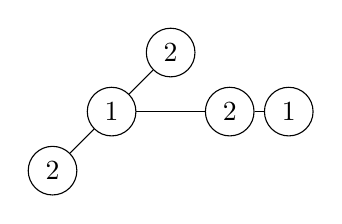
\begin{tikzpicture}[scale=0.75]

            % Noeuds
            \node[circle, draw] (A) at (0,0) {1};
            \node[circle, draw] (B) at (1,1) {2};
            \node[circle, draw] (C) at (-1,-1) {2};
            \node[circle, draw] (D) at (2,0) {2};
            \node[circle, draw] (E) at (3,0) {1};

            % Arêtes
            \draw (A) -- (B);
            \draw (A) -- (C);
            \draw (A) -- (D);
            \draw (D) -- (E);

            \end{tikzpicture}
            
        \end{center}

    \item[$\blacktriangleright$] \textbf{Principes Généraux en PLNE} :
        Soient un problème de \textbf{minimisation} en 
        programmation linéaire dénoté $P$ et sa relaxation continue, 
        $\tilde{P}$. La \textbf{relaxation continue} est obtenue en 
        \textbf{ignorant certaines contraintes}  imposées par 
        le contexte de $P$. 

    \begin{enumerate}
        \item[$\rhd$] \textbf{Relaxation Continue} :
        \begin{itemize}
            \item[$\rhd$] En relâchant les contraintes d'intégralité, on obtient une borne inférieure sur la valeur optimale.
            \item[$\rhd$] Le domaine faisable de la PLNE est inclus dans celui de sa relaxation :
            \[
            F(P) \subseteq F(\tilde{P})
            \]
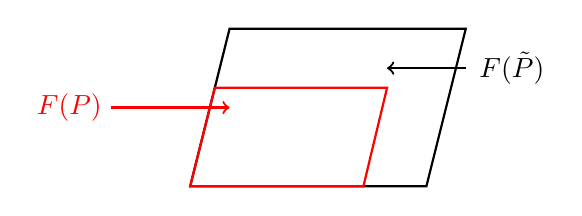
\begin{tikzpicture}

% Outer quadrilateral
\draw[thick] (0,0) -- (3,0) -- (3.5,2) -- (0.5,2) -- cycle;

% Inner quadrilateral (red)
\draw[red, thick] (0,0) -- (2.2,0) -- (2.5,1.25) -- (0.3125,1.25) -- cycle;

% Red arrow pointing to F(Q)
\draw[->, red, thick] (-1,1) -- (0.5,1);
\node[left, red] at (-1,1) {$F(P)$};

% Black arrow pointing to F(\overline{Q})
\draw[->, thick] (3.5,1.5) -- (2.5,1.5);
\node[right] at (3.55,1.5) {$F(\tilde{P})$};

\end{tikzpicture}
        \item [$\rhd$ ] 
            Si nous minimisons sur un domaine réalisable plus grand 
            $F(\tilde{P})$, qui inclut le plus petit domaine $F(P)$, 
            la valeur optimale de l’objectif ne peut qu’être meilleure 
            ou demeurer la même.
            \[ v(\tilde{P}) \leq v(P) \]
        \end{itemize}
        \item[$\rhd$] \textbf{Optimalité des Solutions Entières} :
        \begin{itemize}
            \item[$\rhd$] Si la solution optimale de la relaxation continue est entière, elle est aussi optimale pour le problème entier.
        \end{itemize}
    \end{enumerate}

    \item[$\blacktriangleright$] \textbf{Exemple Illustratif} :
    \begin{itemize}
        \item[$\rhd$] Considérons le problème :
        \[
        \begin{aligned}
        \text{Minimiser} & \quad z = -x_1 - 5x_2 \\
        \text{sous contraintes} & \quad x_1 + 10x_2 \leq 20 \\
        & \quad x_1 \leq 2 \\
        & \quad x_1, x_2 \geq 0 \text{ et entiers}
        \end{aligned}
        \]
        \item[$\rhd$] La relaxation continue permet de trouver une solution fractionnaire qui sert de borne inférieure.
        \item[$\rhd$] Les solutions obtenues par arrondi ou troncature ne sont pas nécessairement optimales pour le problème entier.
    \end{itemize}
\end{itemize}

\section{Algorithme Branch-and-Bound}

\begin{itemize}
    \item[$\blacktriangleright$] \textbf{Introduction} :
    \begin{itemize}
        \item[$\rhd$] Méthode pour résoudre les problèmes de PLNE en explorant systématiquement les sous-problèmes.
        \item[$\rhd$] Combine des techniques de séparation (branching) et d'évaluation (bounding).
    \end{itemize}

    \item[$\blacktriangleright$] \textbf{Branchement (Branching)} :
    \begin{itemize}
        \item[$\rhd$] Si la solution optimale de la relaxation est fractionnaire, on crée deux sous-problèmes en imposant des contraintes supplémentaires sur une variable fractionnaire \( x_j \) :
        \[
        \begin{aligned}
            & P_1 : x_j \leq \lfloor x_j^* \rfloor \\
            & P_2 : x_j \geq \lceil x_j^* \rceil
        \end{aligned}
        \]
    \end{itemize}

    \item[$\blacktriangleright$] \textbf{Évaluation des Sous-Problèmes (Bounding)} :
    \begin{itemize}
        \item[$\rhd$] Résolution de la relaxation continue de chaque sous-problème pour obtenir une borne inférieure.
        \item[$\rhd$] Mise à jour de la borne supérieure \( \overline{z} \) lorsque des solutions entières meilleures sont trouvées.
        \item[$\rhd$] \textbf{Relation des Bornes} :
        \[
        \overline{z} \geq z^* \geq z, \quad \forall \text{ sous-problèmes}
        \]
    \end{itemize}

    \item[$\blacktriangleright$] \textbf{Critères d'Arrêt} :
    \begin{itemize}
        \item[$\rhd$] Un sous-problème peut être éliminé si :
        \begin{itemize}
            \item[$\rhd$] Son domaine faisable est vide.
                \begin{align*}
                    \overline{z}_{P_i} = \{ \}
                \end{align*}
            \item[$\rhd$] La solution optimale est entière et son coût est supérieur ou égal à \( \overline{z} \).
                \begin{align*}
                    \forall \;\; x_{ij} \; : \; x_{ij} \in {N}, \; 
                    \overline{z}_{P_i} \geq \overline{z}_{\text{courrant}}
                \end{align*}
            \item[$\rhd$] La borne inférieure du sous-problème est supérieure ou égale à \( \overline{z} \).
                \begin{align*}
                \overline{z}_{P_i} \geq \overline{z}_{\text{courrant}} 
                \end{align*}            
        \end{itemize}
    \end{itemize}

    \item[$\blacktriangleright$] \textbf{Algorithme (Pseudo-Code)} :
    \begin{enumerate}
        \item \textbf{Initialisation} : Résoudre la relaxation continue du problème initial pour obtenir une borne inférieure \( z \).
        \item \textbf{Mise à Jour} :
        \begin{itemize}
            \item[$\rhd$] Si la solution est entière, elle devient la borne supérieure \( \overline{z} \).
            \item[$\rhd$] Sinon, on branche sur une variable fractionnaire pour créer des sous-problèmes.
        \end{itemize}
        \item \textbf{Exploration} :
        \begin{itemize}
            \item[$\rhd$] Résoudre les relaxations continues des sous-problèmes.
            \item[$\rhd$] Appliquer les critères d'arrêt pour éliminer des branches.
            \item[$\rhd$] Mettre à jour \( \overline{z} \) si une meilleure solution entière est trouvée.
        \end{itemize}
        \item \textbf{Itération} : Répéter l'exploration jusqu'à ce que toutes les branches soient explorées ou éliminées.
    \end{enumerate}

    \item[$\blacktriangleright$] \textbf{Exemple Illustratif} :
    \begin{itemize}
        \item[$\rhd$] Considérons le problème :
        \[
        \begin{aligned}
        \text{Minimiser} & \quad z = -x_1 - 5x_2 \\
        \text{sous contraintes} & \quad x_1 + 10x_2 \leq 20 \\
        & \quad x_1 \leq 2 \\
        & \quad x_1, x_2 \geq 0 \text{ et entiers}
        \end{aligned}
        \]
        \item[$\rhd$] \textbf{Étape 1} : Résoudre la relaxation continue pour obtenir \( x_1^* = 2 \), \( x_2^* = 1.8 \), \( z^* = -11 \).
        \item[$\rhd$] \textbf{Branchement sur \( x_2 \)} :
        \begin{itemize}
            \item[$\rhd$] \textbf{Sous-problème \( P_1 \)} : \( x_2 \leq 1 \).
            \item[$\rhd$] \textbf{Sous-problème \( P_2 \)} : \( x_2 \geq 2 \).
        \end{itemize}
        \item[$\rhd$] \textbf{Résolution de \( P_1 \)} :
        \begin{itemize}
            \item[$\rhd$] Solution entière : \( x_1 = 2 \), \( x_2 = 1 \), \( z = -7 \).
            \item[$\rhd$] Mise à jour de \( \overline{z} = -7 \).
        \end{itemize}
        \item[$\rhd$] \textbf{Résolution de \( P_2 \)} :
        \begin{itemize}
            \item[$\rhd$] Solution entière : \( x_1 = 0 \), \( x_2 = 2 \), \( z = -10 \).
            \item[$\rhd$] Mise à jour de \( \overline{z} = -10 \) car meilleure que la précédente.
        \end{itemize}
        \item[$\rhd$] \textbf{Conclusion} : La solution optimale est \( x_1 = 0 \), \( x_2 = 2 \), avec \( z = -10 \).
    \end{itemize}
\end{itemize}
\begin{tikzpicture}[scale=0.9]

% Coloration de la région
\filldraw[fill=orange, fill opacity=0.7] (0,0) -- (0,1) -- (2,1) -- (2,0) -- cycle;

% Axes
\draw[->] (-0.5,0) -- (3,0) node[below] {$x_1$};
\draw[->] (0,-0.5) -- (0,3) node[left] {$x_2$};

% Étiquettes des axes
\node at (2,-0.2) {2};
\node at (-0.2,2) {2};

% Les lignes contraintes
\draw[dashed, myg] (-2,0.4) -- (1.75,-0.35) node[below left] {$-x_1 - 5x_2 = 0$};
\draw[myb] (2,0) -- (2,2.5) node[above right] {$x_1 = 2$};
\draw[myb] (0,2) -- (3.5, 2) node[above right] {$x_2 = 2$};
\draw[myb] (0,1) -- (3.5, 1) node[right] {$x_2 = 1$};
\draw[myb] (0,2) -- (3.5, 1.65) node[right] {$x_1 + 10x_2 = 20$};
% Les points
\filldraw[black] (2,1.8) circle (2pt);
\filldraw[red] (1,1) circle (2pt);
\filldraw[red] (0,1) circle (2pt);
\filldraw[red] (1,0) circle (2pt);
\filldraw[red] (2,1) circle (2pt);
\filldraw[red] (0,2) circle (2pt);
\filldraw[red] (0,0) circle (2pt);
\filldraw[red] (2,0) circle (2pt);

% Légende point (2,9/5)
\node[left] at (-0.2,11/5) {\textcolor{myr}{$F(\overline{P_2}) = \{ (0, 2) \}$}};

% Le label de F(\overline{P})
\node at (1,0.6) {\textcolor{black}{$F(\overline{P}_1)$}};
\end{tikzpicture}


\blankpage


\chapter{Optimisation de Graphes et Réseaux 1}

\section{Notions de Base}

\begin{itemize}
    \item[$\blacktriangleright$] \textbf{Graphe Non Orienté} :
    \begin{itemize}
        \item[$\rhd$] Un graphe \( G = (V, E) \) où \( V \) est l'ensemble des sommets et \( E \) l'ensemble des arêtes.
        \item[$\rhd$] Une arête \( (i, j) \) relie les sommets \( i \) et \( j \).
        \item[$\rhd$] Deux sommets sont \textbf{adjacents} s'ils sont reliés par une arête.
        \item[$\rhd$] Une arête est \textbf{incidente} à ses sommets.

        \begin{center}
    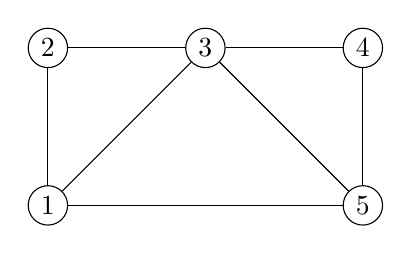
\begin{tikzpicture}[scale=1, every node/.style={circle, draw, minimum size=.5cm, inner sep=0pt}]

    % Nodes
    \node (1) at (0,0) {1};
    \node (2) at (0,2) {2};
    \node (3) at (2,2) {3};
    \node (4) at (4,2) {4};
    \node (5) at (4,0) {5};

    % Edges
    \draw (1) -- (2);
    \draw (1) -- (3);
    \draw (2) -- (3);
    \draw (3) -- (4);
    \draw (3) -- (5);
    \draw (1) -- (5);
    \draw (5) -- (4);

    \end{tikzpicture}
        \item [$\blacktriangleright$ ] 
            Ici, $V = \{ 1, 2, 3, 4, 5\}$
        \end{center}                    
        \item [$\blacktriangleright$ ] 
            $E = \{(1,2), \; (1,3),  \; (1,5), (2,3), (3, 4), (4, 5) \}$ 
    \end{itemize}
\item[$\blacktriangleright$] \textbf{Chaînes et Cycles} :
    \begin{itemize}
        \item[$\rhd$] Une \textbf{chaîne} est une suite d'arêtes 
            $e_1, e_2, \dots, e_p$ connectant une séquence de sommets où 
            il existe $p+1$ \textbf{sommets} $v_1, v_2, \dots, v_{p+1}$  
        \begin{center}
        \begin{tikzpicture}[scale=1, every node/.style={circle, draw, minimum size=.5cm, inner sep=0pt}]

        % Nodes
        \node (1) at (0,0) {1};
        \node (2) at (0,2) {2};
        \node (3) at (2,2) {3};
        \node (4) at (4,2) {4};
        \node (5) at (4,0) {5};

        % Edges
        \draw[thick, myr] (1) -- (2);
        \draw (1) -- (3);
        \draw[thick, myr] (2) -- (3);
        \draw (3) -- (4);
        \draw (3) -- (5);
        \draw (1) -- (5);
        \draw (5) -- (4);

        \end{tikzpicture}
        \item [$\blacktriangleright$ ] 
            Ici, $(1,2), (2,3)$ est une \textbf{chaîne}  
        \item [$\blacktriangleright$ ] 
            $p = 2, \;  e_1 = (1,2), \;  e_2 = (2,3),  
            \; v_1 = 1, v_2 = 2, v_3 = 3 $
        \end{center}                
        \item[$\rhd$] Un \textbf{cycle} est une chaîne où le premier et le dernier sommet sont identiques.
        \begin{center}
        \begin{tikzpicture}[scale=1, every node/.style={circle, draw, minimum size=.5cm, inner sep=0pt}]

        % Nodes
        \node (1) at (0,0) {1};
        \node (2) at (0,2) {2};
        \node (3) at (2,2) {3};
        \node (4) at (4,2) {4};
        \node (5) at (4,0) {5};

        % Edges
        \draw[thick, myr] (1) -- (2);
        \draw[thick, myr] (1) -- (3);
        \draw[thick, myr] (2) -- (3);
        \draw (3) -- (4);
        \draw (3) -- (5);
        \draw (1) -- (5);
        \draw (5) -- (4);

        \end{tikzpicture}
        \item [$\blacktriangleright$ ] 
            Ici, $(1,2), (2,3), (1,3) $ est une \textbf{cycle}  
        \end{center}
    \end{itemize}
    \item[$\blacktriangleright$] \textbf{Graphe Connexe} :
    \begin{itemize}
        \item[$\rhd$] Un graphe est connexe s'il existe une chaîne entre chaque paire de sommets.
    \end{itemize}
\end{itemize}

\subsection{Graphe Orienté et Concepts Associés}

\begin{itemize}
    \item[$\blacktriangleright$] \textbf{Graphe Orienté} :
    \begin{itemize}
        \item[$\rhd$] Un graphe \( G = (V, A) \) où \( A \) est l'ensemble des arcs (arêtes orientées).
        \item[$\rhd$] Un arc \( (i, j) \) va du sommet \( i \) au sommet \( j \).
    \end{itemize}
    \begin{center}
            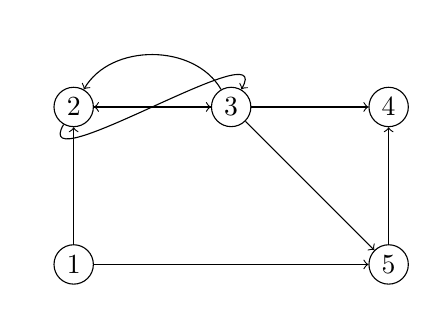
\begin{tikzpicture}[scale=1, every node/.style={circle, draw, minimum size=0.5cm, inner sep=0pt}]

            % Nodes
            \node (1) at (0,0) {1};
            \node (2) at (0,2) {2};
            \node (3) at (2,2) {3};
            \node (4) at (4,2) {4};
            \node (5) at (4,0) {5};

            % Edges (directed)
            \draw[->] (1) -- (2);
            \draw[->] (2) -- (3);
            \draw[->] (3) -- (2);
            \draw[->] (3) -- (4);
            \draw[->] (3) -- (5);
            \draw[->] (1) -- (5);
            \draw[->] (5) -- (4);

            % Loop on node 3
            \draw[->] (2) to[in=60, out=-120] (3);
            \draw[->] (3) to[out=120,in=60] (2);
            \end{tikzpicture}
        
    \end{center}
    \item[$\blacktriangleright$] \textbf{Chemins et Circuits} :
    \begin{itemize}
        \item[$\rhd$] Un \textbf{chemin} est une suite d'arcs orientés dans la même direction.
        \item[$\rhd$] Un \textbf{circuit} est un chemin fermé (départ et arrivée au même sommet).
    \end{itemize}
    \begin{center}
            \begin{tikzpicture}[scale=1, every node/.style={circle, draw, minimum size=0.5cm, inner sep=0pt}]

            % Nodes
            \node (1) at (0,0) {1};
            \node (2) at (0,2) {2};
            \node (3) at (2,2) {3};
            \node (4) at (4,2) {4};
            \node (5) at (4,0) {5};

            % Edges (directed)
            \draw[thick, myr, ->] (1) -- (2);
            \draw[thick, myr, ->] (2) -- (3);
            \draw[->] (3) -- (2);
            \draw[->] (3) -- (4);
            \draw[thick, myr, ->] (3) -- (5);
            \draw[->] (1) -- (5);
            \draw[->] (5) -- (4);

            % Loop on node 3
            \draw[->] (2) to[in=60, out=-120] (3);
            \draw[->] (3) to[out=120,in=60] (2);
            \end{tikzpicture}
        
    \end{center}
\end{itemize}

\subsection{Concepts de Flot et Contraintes sur les Arcs}

\begin{itemize}
    \item[$\blacktriangleright$] \textbf{Flot sur les Arcs} :
    \begin{itemize}
        \item[$\rhd$] Chaque arc \( (i, j) \) a :
        \begin{itemize}
            \item[$\rhd$] Une \textbf{borne inférieure} \( l_{ij} \) (minimum de flot).
            \item[$\rhd$] Une \textbf{capacité} \( u_{ij} \) (maximum de flot).
            \item[$\rhd$] Un \textbf{coût} \( c_{ij} \) par unité de flot.
        \end{itemize}
    \end{itemize}
    \item[$\blacktriangleright$] \textbf{Objectif} :
    \begin{itemize}
        \item[$\rhd$] Maximiser le flot total du \textbf{source} \( s \) au \textbf{puits} \( t \).
        \item[$\rhd$] Minimiser le coût total associé au flot.
    \end{itemize}
\end{itemize}

\section{Problèmes de Flots à Coût Minimal}

\subsection{Notations de Base}

\begin{itemize}
    \item[$\rhd$] \( G = (V, A) \) : Graphe orienté avec sommets \( V \) et arcs \( A \).
    \item[$\rhd$] \( c_{ij} \) : Coût par unité de flot sur l'arc \( (i, j) \).
    \item[$\rhd$] \( x_{ij} \) : Flot sur l'arc \( (i, j) \).
    \item[$\rhd$] \( u_{ij} \) : Capacité maximale de l'arc \( (i, j) \).
    \item[$\rhd$] \( s \) : Source du réseau.
    \item[$\rhd$] \( t \) : Puits du réseau.
    \item [$\rhd$ ] $B_i$ : ensemble des arcs entrants dans $i$ : $(j,i)$
    \item [$\rhd$ ] $P_i$ : ensemble des arcs sortant de  $i$ : $(i, j)$
\end{itemize}
\subsection{Diagramme pour \( B_i \) et \( P_i \)}

\begin{center}
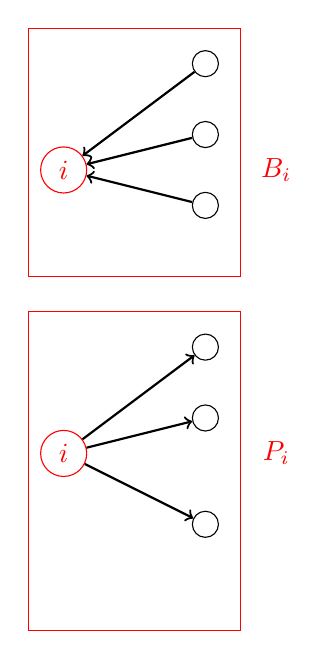
\begin{tikzpicture}[scale=0.9]

% Sommets du graphe
\node[draw, circle, red] (i) at (0,0) {$i$};
\node[draw, circle] (v1) at (2,1.5) {};
\node[draw, circle] (v2) at (2,0.5) {};
\node[draw, circle] (v3) at (2,-0.5) {};

% Arcs pour Bi
\draw[->, thick] (v1) -- (i);
\draw[->, thick] (v2) -- (i);
\draw[->, thick] (v3) -- (i);

% Cadre pour Bi
\draw[red] (-0.5,2) rectangle (2.5,-1.5);
\node[red] at (3, 0) {$B_i$};

% Sommets du graphe pour Pi
\node[draw, circle, red] (i2) at (0,-4) {$i$};
\node[draw, circle] (v4) at (2,-2.5) {};
\node[draw, circle] (v5) at (2,-3.5) {};
\node[draw, circle] (v6) at (2,-5) {};

% Arcs pour Pi
\draw[->, thick] (i2) -- (v4);
\draw[->, thick] (i2) -- (v5);
\draw[->, thick] (i2) -- (v6);

% Cadre pour Pi
\draw[red] (-0.5,-2) rectangle (2.5,-6.5);
\node[red] at (3, -4) {$P_i$};

\end{tikzpicture}
\end{center}

\subsection{Formulation Mathématique}

\begin{alignat*}{4}
&\text{Minimiser} \quad & z = \sum_{(i,j) \in A} c_{ij} x_{ij} 
\\
\\
&\text{sous contraintes} \quad & \sum_{j \in P_i} x_{ij} - \sum_{j \in B_i} x_{ji} =
\begin{cases}
d & \text{si } i = s \\
-d & \text{si } i = t \\
0 & \text{sinon}
\end{cases} \\
& & l_{ij} \leq x_{ij} \leq u_{ij}, \quad \forall (i,j) \in A
\end{alignat*}

\begin{itemize}
    \item[$\rhd$] \( P_i \) : Ensemble des sommets atteints depuis \( i \) (arcs sortants).
    \item[$\rhd$] \( B_i \) : Ensemble des sommets rejoignant \( i \) (arcs entrants).
    \item[$\rhd$] \( d \) : Quantité de flot à acheminer de \( s \) vers \( t \).
\end{itemize}

\subsection{Interprétation}

\begin{itemize}
    \item[$\blacktriangleright$] \textbf{Conservation du Flot} : Le flot entrant moins le flot sortant est égal à la demande ou l'offre en chaque sommet.
    \item[$\blacktriangleright$] \textbf{Respect des Capacités} : Le flot sur chaque arc doit respecter ses bornes.
    \item[$\blacktriangleright$] \textbf{Objectif} : Minimiser le coût total du transport du flot.
\end{itemize}

\section{Exemple de Problème à Coût Minimal}
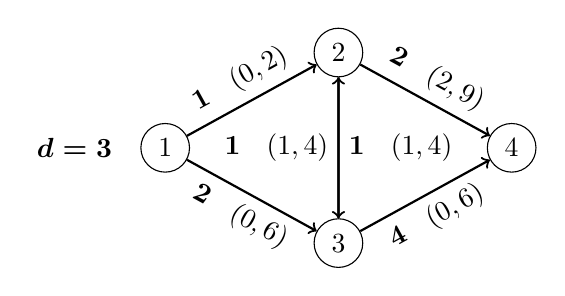
\begin{tikzpicture}[scale=1.1]

% Nodes (vertices)
\node[draw, circle] (1) at (0, 0) {1};
\node[draw, circle] (2) at (2, 1.1) {2};
\node[draw, circle] (3) at (2, -1.1) {3};
\node[draw, circle] (4) at (4, 0) {4};

% Arrows and labels
\draw[->, thick] (1) -- (2) node[midway, above, sloped] {$\boldsymbol{1}$ \; $(0,2)$};
\draw[->, thick] (1) -- (3) node[midway, below, sloped] {$\boldsymbol{2}$  \; $(0,6)$};
\draw[->, thick] (2) -- (4) node[midway, above, sloped] {$\boldsymbol{2}$ \; $(2,9)$};
\draw[->, thick] (3) -- (4) node[midway, below, sloped] {$\boldsymbol{4}$ \; $(0,6)$};
\draw[->, thick] (2) -- (3) node[midway, right] {$\boldsymbol{1}$   \; $(1,4)$};
\draw[->, thick] (3) -- (2) node[midway, left] {$\boldsymbol{1}$ \; $(1,4)$};

% Flow value
\node[left] at (-0.5, 0) {$\boldsymbol{d = 3}$};

\end{tikzpicture}
\begin{itemize}
    \item[$\blacktriangleright$] \textbf{Réseau} :
    \begin{itemize}
        \item[$\rhd$] Sommets : 1 (source), 2, 3 (intermédiaire), 4 (puits).
        \item[$\rhd$] Arcs avec coûts \( c_{ij} \), capacités \( u_{ij} \) et bornes inférieures \( l_{ij} \).
    \end{itemize}
    \item[$\blacktriangleright$] \textbf{Objectif} :
    \[
    \text{Minimiser} \quad z = x_{12} + 2x_{13} + 2x_{23} + 2x_{24} + x_{32} + 4x_{34}
    \]
    \item[$\blacktriangleright$] \textbf{Contraintes de Conservation du Flot} :
    \[
    \begin{cases}
    x_{12} + x_{13} = 3 & \text{(sommet 1)} \\
    -x_{12} + x_{23} + x_{24} - x_{32} = 0 & \text{(sommet 2)} \\
    -x_{13} - x_{23} + x_{32} + x_{34} = 0 & \text{(sommet 3)} \\
    -x_{24} - x_{34} = -3 & \text{(sommet 4)}
    \end{cases}
    \]
    \item[$\blacktriangleright$] \textbf{Contraintes de Capacité et Bornes} :
    \[
    \begin{aligned}
    & 0 \leq x_{12} \leq 2, \quad 0 \leq x_{13} \leq 4, \quad 0 \leq x_{23} \leq 6, \\
    & 2 \leq x_{24} \leq 9, \quad 1 \leq x_{32} \leq 4, \quad 0 \leq x_{34} \leq 6
    \end{aligned}
    \]
\end{itemize}

\section{Problème de Flot avec Plusieurs Sources et Puits}

    \subsection{Formulation Générale}
        \begin{itemize}
            \item[$\rhd$] \textbf{Objectif} :
            \[%
            \text{Minimiser} \quad z = \sum_{(i,j) \in A} c_{ij} x_{ij}
            \]%
            \item[$\rhd$] \textbf{Contraintes de Conservation du Flot} :
            \[%
            \sum_{j \in P_i} x_{ij} - \sum_{j \in B_i} x_{ji} =
                \begin{cases}
                     d_i & \text{si } i \in S \ (\text{sources}) \\
                    -d_j & \text{si } i \in T \ (\text{puits}) \\
                      0 & \text{sinon}
                \end{cases}
            \]%
            \item[$\rhd$] \textbf{Contraintes de Capacité} :
            \[%
            0 \leq x_{ij} \leq u_{ij}, \quad \forall (i,j) \in A
            \]%
        \end{itemize}

        \subsection{Interprétation}

        \begin{itemize}
            \item[$\blacktriangleright$] Chaque source \( s_i \) fournit un flot \( d_i \).
            \item[$\blacktriangleright$] Chaque puits \( t_j \) consomme un flot \( d_j \).
            \item[$\blacktriangleright$] Le flot total injecté par les sources est 
                                    égal au flot total absorbé par les puits :
            \[%
            \sum_{i \in S} d_i = \sum_{j \in T} d_j
            \]%
        \end{itemize}

\section{Problème de Flot à Coût Maximal avec Arc Fictif}
    \subsection{Approche}

        \begin{itemize}
            \item[$\blacktriangleright$] Introduction d'un \textbf{arc fictif} \( (t, s) \) avec :
                \begin{itemize}
                    \item[$\rhd$] Capacité infinie.
                    \item[$\rhd$] Coût \( c_{ts} = -1 \).
                \end{itemize}
            \item[$\blacktriangleright$] \textbf{Objectif} :
            \[%
                \text{Minimiser} \quad z = \sum_{(i,j) \in A} c_{ij} x_{ij} - x_{ts}
            \]%
            \item[$\blacktriangleright$] Ceci équivaut à \textbf{maximiser} \( x_{ts} \), le flot total du réseau.
        \end{itemize}

    \subsection{Formulation Mathématique}

\begin{align*}
\text{Minimiser} \quad & z = \sum_{(i,j) \in A} c_{ij} x_{ij} - x_{ts} \\
\text{sous contraintes} \quad & \sum_{j \in P_i} x_{ij} - \sum_{j \in B_i} x_{ji} = 0, \quad \forall i \in V \\
& x_{ij} \geq l_{ij}, \quad x_{ij} \leq u_{ij}, \quad \forall (i,j) \in A^+ \\
& x_{ts} \geq 0
\end{align*}

\subsection{Interprétation}

\begin{itemize}
    \item[$\blacktriangleright$] L'arc fictif \( (t, s) \) permet de transformer le problème en un problème de minimisation avec une fonction objectif linéaire.
    \item[$\blacktriangleright$] Maximiser le flot sur \( x_{ts} \) revient à maximiser le flot total dans le réseau.
\end{itemize}
\section{Algorithme de Dijkstra}

\subsection{Introduction}

L'algorithme de Dijkstra est une méthode efficace pour trouver les chemins les plus courts depuis un sommet source \( s \) vers tous les autres sommets dans un graphe connexe non orienté et pondéré \( G = (V, E) \). Les poids des arêtes représentent les distances ou les coûts, et doivent être non négatifs.

\subsection{Notations et Ensembles}

\begin{itemize}
    \item[\( \lambda_{ij} \)] : Longueur (ou poids) de l'arête entre les sommets \( i \) et \( j \), avec \( \lambda_{ij} \geq 0 \).
    \item[\( N_i \)] : Ensemble des voisins (sommets adjacents) du sommet \( i \):
        \[
            N_i = \{ j \in V \mid (i, j) \in E \}
        \]
    \item[\( EM \)] : Ensemble des sommets marqués, c'est-à-dire les sommets pour lesquels le chemin le plus court depuis \( s \) a été déterminé.
    \item[\( EM^c \)] : Complémentaire de \( EM \), soit l'ensemble des sommets non marqués :
        \[
            EM^c = V \setminus EM
        \]
    \item[\( \delta_j \)] : Étiquette associée au sommet \( j \), représentant la longueur du chemin le plus court de \( s \) à \( j \) trouvé jusqu'à présent.
\end{itemize}

\subsection{Étapes de l'Algorithme}

\begin{enumerate}
    \item \textbf{Initialisation} :
        \begin{itemize}
            \item[\( \rhd \)] Définir \( EM = \{ s \} \) et initialiser \( \delta_s = 0 \).
            \item[\( \rhd \)] Pour tout \( j \in V \setminus \{ s \} \), initialiser \( \delta_j = +\infty \).
        \end{itemize}

    \item \textbf{Étape Itérative} : Tant que \( EM^c \neq \emptyset \), répéter les sous-étapes suivantes :

        \begin{enumerate}
            \item \textbf{Trouver le sommet adjacent le plus proche} :
                \begin{itemize}
                    \item[\( \rhd \)] Pour chaque \textbf{sommet  marqué}  \( i \in EM \), 
                         trouver le sommet $j$ \textbf{non marqué} qui est adjacent à 
                         $i$ et qui est \textbf{le plus proche de } $i$  :
                        \[
                            \min_{j \in EM^c \cap \; N_i}\bigl\{\lambda_{ij} \bigr\}
                        \]
                \end{itemize}

            \item \textbf{identifier le sommet adjacent} :
                \begin{itemize}
                    \item[\( \rhd \)] 
                        Pour chaque $i \in EM$ pour lequel on a trouvé le 
                        sommet adjacent $j$ le plus proche, 
                        marquer 
                        \[
                            \boxed{j_i = j}
                        \]
\begin{center}
    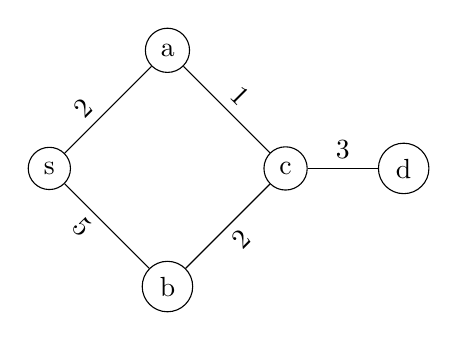
\begin{tikzpicture}[scale=0.75]
        % Définition d'un style pour les sommets
        \tikzstyle{sommet}=[circle, draw, minimum size=0.5cm]

        % Nœuds
        \node[sommet] (s) at (0, 0) {s};
        \node[sommet] (a) at (2, 2) {a};
        \node[sommet] (b) at (2, -2) {b};
        \node[sommet] (c) at (4, 0) {c};
        \node[sommet] (d) at (6, 0) {d};

        % Arcs avec poids
        \draw (s) -- node[above left, sloped] {2} (a);
        \draw (s) -- node[below left, sloped] {5} (b);
        \draw (a) -- node[above, sloped] {1} (c);
        \draw (b) -- node[below, sloped] {2} (c);
        \draw (c) -- node[above, sloped] {3} (d);
    \end{tikzpicture}
\end{center}
    \item [$\blacktriangleright$ ] \textbf{Exemple}. Soit $s \in EM$, on a :

        \begin{align*}
            j_s = \min\bigl\{\lambda_{sa}, \lambda_{sb} \bigr\} = 
            \min\bigl\{2, 5 \bigr\} = 2
        \end{align*}

    \item [$\blacktriangleright$ ] \textbf{Identification}. 
        Donc on identifie:
        \begin{align*}
            j_s = a
        \end{align*}
                \end{itemize}

            \item \textbf{Trouver la chaîne la plus courte} :
                \begin{itemize}
                    \item [$\rhd$ ] Pour chaque sommet \textbf{marqué}, trouver 
                        la chaîne la plus courte :
                        \[
                           \Delta = \min_{i\in EM}\bigl\{\delta_i + \lambda_{ij_i} \bigr\}
                        \]
            \end{itemize}
        \item \textbf{Marquer le sommet créant la chaîne la plus courte} :
        \begin{itemize}
            \item [$\rhd$ ] Lorsqu'on trouve le \textbf{sommet} $j$ 
                créant la chaîne la plus courte, on le marque :
                \begin{align*}
                    \delta_j = \Delta
                \end{align*}
    \item [$\blacktriangleright$ ] \textbf{Exemple}. Soit $s \in EM$, 
        $j_s = a$, $\delta_s = 0$, on a :

        \begin{align*}
            \min\bigl\{\lambda_{sa}, \lambda_{sb} \bigr\} = 
            \min\bigl\{0 + 2 \bigr\} = 2 = \Delta
        \end{align*}

    \item [$\blacktriangleright$ ] \textbf{Marquage}. 
        Donc on marque :
        \begin{align*}
            \delta_a  = 2
        \end{align*}

                \end{itemize}
        \end{enumerate}

    \item \textbf{Terminaison} :
        \begin{itemize}
            \item[\( \rhd \)] Lorsque tous les sommets sont marqués (\( EM = V \)), l'algorithme s'arrête. Les étiquettes \( \delta_j \) contiennent alors les longueurs minimales des chemins depuis \( s \) vers chaque sommet \( j \).
        \end{itemize}
\end{enumerate}

\subsection{Remarques Importantes}

\begin{itemize}
    \item[\( \blacktriangleright \)] L'algorithme de Dijkstra fonctionne correctement uniquement si tous les poids des arêtes \( \lambda_{ij} \) sont non négatifs.
    \item[\( \blacktriangleright \)] Il peut être adapté aux graphes orientés en considérant les arcs orientés au lieu des arêtes.
    \item[\( \blacktriangleright \)] L'efficacité de l'algorithme peut être améliorée en utilisant des structures de données appropriées, comme des files de priorité (tas).
\end{itemize}

\subsection{Exemple Illustratif}

\begin{center}
    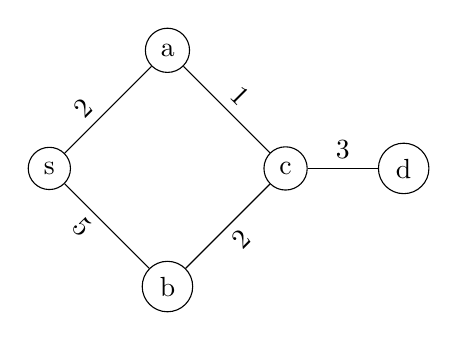
\begin{tikzpicture}[scale=0.75]
        % Définition d'un style pour les sommets
        \tikzstyle{sommet}=[circle, draw, minimum size=0.5cm]

        % Nœuds
        \node[sommet] (s) at (0, 0) {s};
        \node[sommet] (a) at (2, 2) {a};
        \node[sommet] (b) at (2, -2) {b};
        \node[sommet] (c) at (4, 0) {c};
        \node[sommet] (d) at (6, 0) {d};

        % Arcs avec poids
        \draw (s) -- node[above left, sloped] {2} (a);
        \draw (s) -- node[below left, sloped] {5} (b);
        \draw (a) -- node[above, sloped] {1} (c);
        \draw (b) -- node[below, sloped] {2} (c);
        \draw (c) -- node[above, sloped] {3} (d);
    \end{tikzpicture}

\end{center}

\begin{itemize}
    \item[\( \rhd \)] \textbf{Initialisation} :
        \begin{itemize}
            \item[\( \bullet \)] \( EM = \{ s \} \), \( \delta_s = 0 \), \( \delta_a = \delta_b = \delta_c = \delta_d = +\infty \).
        \end{itemize}
    \item[\( \rhd \)] \textbf{Itération 1} :
        \begin{itemize}
            \item[\( \bullet \)] \circled{$s$} :
                \[
                    \min(\lambda_{sa}, \lambda_{sb}) = 
                    \min(\boldsymbol{2}   , 5) = 2 \implies j_s = a
                \]
            \item[\( \bullet \)] Chaîne la plus courte :
                \begin{align*}
                    \Delta &= \min\bigl( \delta_s + \lambda_{sa} \bigr) \\
                      &= \min\bigl( 0 + 2 \bigr) = 2  \\
                      &\implies \delta_a = 2
                \end{align*}
        \end{itemize}
    \item[\( \rhd \)] \textbf{Itération 2} :
        \begin{itemize}
            \item[\( \bullet \)] \( EM = \{ s, a \} \), \( \delta_s = 0, \delta_a = 2\), \( \delta_b = \delta_c = \delta_d = +\infty \).
            \item[\( \bullet \)]  \circled{$s$}:
                \[
                    \min(\lambda_{sa}, \lambda_{sb}) = 
                    \min(\boldsymbol{5}  ) = 5 \implies j_s = b
                \]
            \item[\( \bullet \)]  \circled{$a$}:
                \[
                    \min(\lambda_{ac}, \lambda_{as}) =  
                    \min(\boldsymbol{1}, 2) = 1 \implies j_a = c
                \]
            \item[\( \bullet \)] Chaîne la plus courte :
                \begin{align*}
                    \Delta &= \min\bigl( \delta_s + \lambda_{sb}, \delta_a + \lambda_{ac} \bigr) \\
                           &= \min\bigl( 0 + 5, 2 + 1 \bigr) = 3  \\ 
                           &\implies \delta_c = 3 
                \end{align*}
        \end{itemize}

    \item[\( \rhd \)] \textbf{Itération 3} :
        \begin{itemize}
            \item[\( \bullet \)] \( EM = \{ s, a, c \} \), \( \delta_s = 0, \delta_a = 2, \delta_c = 3\), \( \delta_b = \delta_d = +\infty \).
            \item[\( \bullet \)]  \circled{$c$}:
                \[
                    \min(\lambda_{c_b}, \lambda_{cd}) =  
                    \min(\boldsymbol{2}, 3  ) = 2 \implies j_c = b
                \]
            \item[\( \bullet \)] Chaîne la plus courte :
                \begin{align*}
                    \Delta &= \min\bigl( \delta_c + \lambda_{cb} \bigr) \\
                           &= \min\bigl( 3 + 2 \bigr) = 5  \\ 
                           &\implies \delta_b = 5 
                \end{align*}
        \end{itemize}  
    \item[\( \rhd \)] \textbf{Itération 4} :
        \begin{itemize}
            \item[\( \bullet \)] \( EM = \{ s, a, c, d \} \), \( \delta_s = 0, \delta_a = 2, \delta_c = 3,  \delta_b= 5\), \(  \delta_d = +\infty \).
            \item[\( \bullet \)]  \circled{$c$}:
                \[
                    \min(\lambda_{cd}) =  
                    \min( \boldsymbol{3}) = 3\implies j_c = d
                \]
            \item[\( \bullet \)] Chaîne la plus courte :
                \begin{align*}
                    \Delta &= \min\bigl( \delta_c + \lambda_{cd} \bigr) \\
                           &= \min\bigl( 3 + 3 \bigr) = 6  \\ 
                           &\implies \delta_d = 6 
                \end{align*}
        \end{itemize} \end{itemize}

        Le chemin le plus court de $s$ à $d$ est $\boldsymbol{\delta_d = 6}$, en 
        visitant, dans l'ordre, les noeud $s, a, c, d$. 

\blankpage



\newpage
\chapter{Optimisation de Graphes et Réseaux 2}
\section{Problème de transport et d'affectation}

\begin{itemize}
    \item [$\blacktriangleright$ ] \textbf{Problème d'affectation}  
        \begin{itemize}
            \item [$\rhd$ ] Cas particulier du problème de 
                \textit{flot à coût minimal} dans lequel on  a plusieurs 
                \textbf{sources} et \textbf{puits}. 
            \item [$\rhd$ ] Un certain nombre de \textbf{ressources} 
                devoient être acheminé des sources \textbf{vers} les puits.   
        \end{itemize}
    \item [$\blacktriangleright$ ] \textbf{Sources} $\boldsymbol{i}$    
        \begin{itemize}
            \item [$\rhd$ ] 
                Chaque source $i \in S$ \textbf{offre} une quantité de ressources 
            $\boldsymbol{o_i}$.   
        \end{itemize}
    \item [$\blacktriangleright$ ] \textbf{Puits} $\boldsymbol{j}$    
        \begin{itemize}
            \item [$\rhd$ ] 
                Chaque puits $j \in T$ \textbf{demande} 
                une quantité de ressources 
            $\boldsymbol{d_j}$.   
        \end{itemize}
    \item [$\blacktriangleright$ ] \textbf{Ensemble des sommets} $\boldsymbol{V}$  
        \begin{itemize}
            \item [$\rhd$ ] 
                Il n'y aucun sommet interminédiaire; il n'y a que les sommets 
                sources et puits :
                \begin{align*}
                    V = S \cup T
                \end{align*}
        \end{itemize}
    \item [$\blacktriangleright$ ] \textbf{Quantité de sommets} dans $\boldsymbol{V}$  
        \begin{itemize}
            \item [$\rhd$ ] 
                Il y a généralement \textbf{plus de demande} que d'offre :
                \begin{align*}
                    |S|  = m \leq n = |T|
                \end{align*}
        \end{itemize}
    \item [$\blacktriangleright$ ] \textbf{Ensemble des arcs} dans $\boldsymbol{A}$  
        \begin{itemize}
            \item [$\rhd$ ] 
                Chaque arc $(i, j) \in A$ mène d'une source 
                $i \in S$ à un puits $j \in T$:
        \end{itemize}
    \item [$\blacktriangleright$ ] \textbf{Poids des arcs} $\boldsymbol{c_{ij}}$  
        \begin{itemize}
            \item [$\rhd$ ] 
                À chaque arc $(i, j) \in A$ est associé un 
                \textbf{coût de transport} ou d'\textbf{association }
                $c_{ij}$  
        \end{itemize}
    \item [$\blacktriangleright$ ] \textbf{Bornes} des arcs 
        \begin{itemize}
            \item [$\rhd$ ] 
                À chaque arc $(i, j) \in A$ est associé une 
                \textbf{bornes} : 
            \item [$\blacktriangleright$ ] \textbf{Borne inférieure} 
                $l_{ij} = 0$; impose une contrainte de non négativité.
            \item [$\blacktriangleright$ ] \textbf{Borne supérieure} 
                $u_{ij} = \infty$
        \end{itemize}
\end{itemize}                           

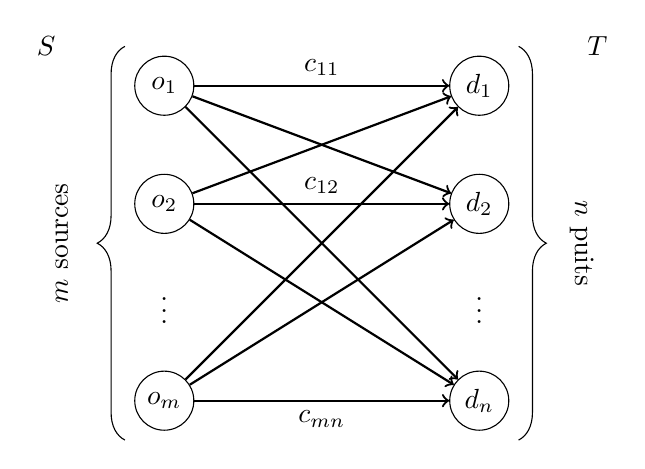
\begin{tikzpicture}[
    source/.style={circle, draw, minimum size=0.75cm, inner sep=0pt},
    sink/.style={circle, draw, minimum size=0.75cm, inner sep=0pt},
    arrow/.style={->, thick}
]

% Sources
\node[source] (o1) at (0,4) {$o_1$};
\node[source] (o2) at (0,2.5) {$o_2$};
\node[source] (om) at (0,0) {$o_m$};
\node at (0,1.25) {$\vdots$};

% Sinks
\node[sink] (d1) at (4,4) {$d_1$};
\node[sink] (d2) at (4,2.5) {$d_2$};
\node[sink] (dn) at (4,0) {$d_n$};
\node at (4,1.25) {$\vdots$};

% Arrows between sources and sinks
\draw[arrow] (o1) -- node[above] {$c_{11}$} (d1);
\draw[arrow] (o1) -- (d2);
\draw[arrow] (o1) -- (dn);
\draw[arrow] (o2) -- (d1);
\draw[arrow] (o2) -- node[above] {$c_{12}$} (d2);
\draw[arrow] (o2) -- (dn);
\draw[arrow] (om) -- (d1);
\draw[arrow] (om) -- (d2);
\draw[arrow] (om) -- node[below] {$c_{mn}$} (dn);

% Labels for braces and texts
\draw[decorate,decoration={brace,amplitude=10pt,mirror}] (-0.5,4.5) -- (-0.5,-0.5) node[midway,xshift=-0.8cm,rotate=90] {$m$ sources};
\draw[decorate,decoration={brace,amplitude=10pt}] (4.5,4.5) -- (4.5,-0.5) node[midway,xshift=0.8cm,rotate=-90] {$n$ puits};

% Label sets S and T
\node at (-1.5,4.5) {$S$};
\node at (5.5,4.5) {$T$};

\end{tikzpicture}

\subsection{Modèle Mathématique}
Pour chaque noeud $i \in S$, il y a $n$ arcs \textbf{sortants}  
potentiels et l'offre pour un noeud $i$ est donné par :

\begin{align*}
    o_i = \sum_{j=1}^{n}c_{ij}x_{ij}
\end{align*}

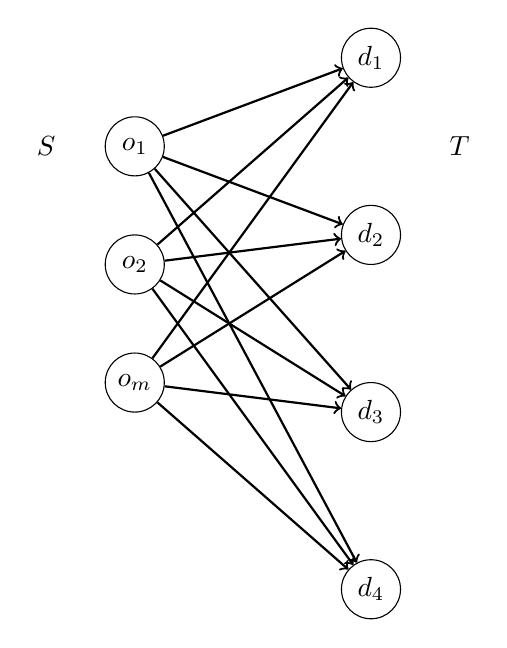
\begin{tikzpicture}[
    source/.style={circle, draw, minimum size=0.75cm, inner sep=0pt},
    sink/.style={circle, draw, minimum size=0.75cm, inner sep=0pt},
    arrow/.style={->, thick},
scale=0.75]

% Sources
\node[source] (o1) at (0,4.5) {$o_1$};
\node[source] (o2) at (0,2.5) {$o_2$};
\node[source] (om) at (0,0.5) {$o_m$};

% Sinks
\node[sink] (d1) at (4,6) {$d_1$};
\node[sink] (d2) at (4,3) {$d_2$};
\node[sink] (d3) at (4,0) {$d_3$};
\node[sink] (dn) at (4,-3) {$d_4$};

% Arrows between sources and sinks
\draw[arrow] (o1) -- (d1);
\draw[arrow] (o1) -- (d2);
\draw[arrow] (o1) -- (d3);
\draw[arrow] (o1) -- (dn);
\draw[arrow] (o2) -- (d1);
\draw[arrow] (o2) -- (d2);
\draw[arrow] (o2) -- (dn);
\draw[arrow] (o2) -- (d3);
\draw[arrow] (om) -- (d1);
\draw[arrow] (om) -- (d2);
\draw[arrow] (om) -- (dn);
\draw[arrow] (om) -- (d3);



% Label sets S and T
\node at (-1.5,4.5) {$S$};
\node at (5.5,4.5) {$T$};

\end{tikzpicture}

\noindent
\textbf{Exemple}  
\begin{align*}
    o_1 = \sum_{j=1}^{n}c_{1j}x_{1j}
\end{align*}

Pour chaque noeud $j\in T$, il y a $n$ arcs \textbf{entrants}   
potentiels et la demande  pour un noeud $i$ est donné par :

\begin{align*}
    d_j = \sum_{i=1}^{m}c_{ij}x_{ij}
\end{align*}

\noindent
\textbf{Exemple}  
\begin{align*}
    d_3 = \sum_{i=1}^{m}c_{i3}x_{i3}
\end{align*}


Pour chaque arc $(i, j) \in A$, on ne peut pas affecter une quantité négative 
de ressources $x_{ij}$ : 

\begin{align*}
    \forall x_{ij} : (i, j) \in A, \; x_{ij} \geq 0
\end{align*}


\begin{align*}
    &\text{Min } z = \sum_{i=1}^{m}\sum_{j=1}^{n}c_{ij}x_{ij}  
    \\ 
    &\text{s.a}
    \\
    &\phantom{\text{Min } z =} 
    \sum_{j =1}^{n} x_{ij} = o_i, \quad i = 1, \cdots, m
    \\
    &\phantom{\text{Min } z =}
    \sum_{i =1}^{m} x_{ij} = d_i, \quad j = 1, \cdots, n
    \\ 
    \\ 
    &x_{ij} \geq 0 \quad (i, j) \in A
\end{align*}

\subsection{Algorithme Hongrois}
\subsection{Introduction}

L'algorithme Hongrois est une \textbf{procédure itérative}  qui permet de résoudre 
des problèmes d'affectation. Il permet d'engendrer 
un \textbf{ensemble de solutions optimales}  qui minimise 
le coût global d'affectation. 

\begin{itemize}
    \item [$\rhd$ ] \textbf{Initialisation} :puits
        Soit un problème d'affectation impliquant $m \in S$ 
        \textbf{sources}  et $n \in T$ \textbf{puits}, produire 
        une matrice $B_{n \times n}$. 
        \begin{itemize}
            \item [$\blacktriangleright$ ] Placer les sources 
                en \textbf{colonnes}  
            \item [$\blacktriangleright$ ] Placer les puits 
                en \textbf{rangées}   
            \item [$\blacktriangleright$ ] S'il y a plus de \textbf{noeud de demande}
                que d'offre, créer une offre fictive en introduisant 
                une rangée de poids nul. 
        \end{itemize}
\end{itemize}

\noindent 
\textbf{Exemple}  
\[\setlength{\arraycolsep}{0pt}
    \begin{NiceArray}{>{\rule[-2.8mm]{0pt}{8mm}}ccccc*{1}{c}}%
  [
    columns-width=8mm ,
    corners = {NW,NE} ,
    hvlines ,
    code-before = \arraycolor{cyan!10}
  ]
   & j_1 & j_2  & j_3  & j_4  \\
        i_1 & 6  &  M  & 3   & 5  \\
i_2 & 8  & 4   & 9   & 6  \\
i_3 & 7 & 5  & 2  & 8  \\
i_f & 0 & 0  & 0  & 0 \\
\end{NiceArray}\]
\begin{itemize}
    \item [$\rhd$ ] \textbf{Étape 1.}  
        \begin{itemize}
            \item [$\blacktriangleright$ ] 
        Dans chacune des \textbf{rangées}, identifier \textbf{le coût minimal}   
        \item [$\blacktriangleright$ ] 
       \textbf{ Soustraire} celui-ci de chacun des coûts dans la rangée 
       correspondante.
        \end{itemize}
    \item [$\rhd$ ] \textbf{Étape 2.}  
        \begin{itemize}
            \item [$\blacktriangleright$ ] 
        Dans chacune des \textbf{colonnes}, identifier \textbf{le coût minimal}   
        \item [$\blacktriangleright$ ] 
       \textbf{ Soustraire} celui-ci de chacun des coûts dans la rangée 
        \end{itemize}
       correspondante.
    \item [$\rhd$ ] \textbf{Étapes 3.}  
        \begin{itemize}
            \item [$\blacktriangleright$ ] 
        Si une \textbf{affectation de coût 0} est possible:
            \begin{itemize}
                \item [$\rhd$ ]  Procéder à cette affectation optimale
                \item [$\rhd$ ] Évaluer son véritable coût 
            avec la matrice des coût originale.
            \end{itemize}
        \end{itemize}
        \end{itemize}

        \begin{note}{}{}
        Une \textbf{affectation de coût 0}   est possible si le nombre minimum de 
        lignes horizontales \textbf{et ou } verticales permettant de couvrir
        \textbf{tous les 0 dans la matrice}  des coûts correspond à la dimension 
        de cette matrice, c'est-à-dire $n$.
        \end{note}

        \noindent 
        \textbf{Exemple}  
\[\setlength{\arraycolsep}{0pt}
    \begin{NiceArray}{>{\rule[-2.8mm]{0pt}{8mm}}cccc*{1}{c}}%
  [
    columns-width=8mm ,
    corners = {NW,NE} ,
    hvlines ,
    code-before = \arraycolor{cyan!10}
  ]
   & j_1 & j_2 & j_3    \\
        i_1 & 0 &  M & 0    \\
i_2 & 4  & 0 & 3       \\
i_3 & 0  & 0 & 0     \\
\CodeAfter
\tikz \draw  [myr, dashed, thick]   (2.5-|2.5) -- (4.5-|2.5)
                                    (2.5-|3.5) -- (4.5-|3.5)
                                    (2.5-|4.5) -- (4.5-|4.5);
\end{NiceArray}\]
Il faut au minimum \textbf{3 lignes }   
horizontales et ou verticales 
pour couvrir tous les 0. La matrice est de dimension $B_{3 \times 3}$ 
Une affectation de coût 0 est donc possible. 

\begin{itemize}
    \item [$\rhd$ ] \textbf{Étape 4.}  
        \begin{itemize}
            \item [$\blacktriangleright$ ] 
                Ajouter des 0 dans la matrice de coût :
                \begin{itemize}
                    \item [$\rhd$ ] 
                    Identifier le plus petit coût non couvert par une ligne.
                    \item [$\rhd$ ] 
                Soustraire ce coût de chacun des coûts non couverts
                par une ligne.
                \item [$\rhd$ ]                                 
                Ajouter ce coût à chacun des coûts couverts 
                par une ligne horizontale et verticale.
                \end{itemize}
        \end{itemize}
    \item [$\rhd$ ] \textbf{Étape 5.} 
        \begin{itemize}
            \item [$\blacktriangleright$ ] Retourner à l’Étape 3.
        \end{itemize}
\end{itemize}


\textbf{À la fin de chaque itération}, 
tant que le nombre lignes horizontales et ou verticales 
nécessaire pour couvrir tous les 0 est inférieur à la dimension de la matrice, 
on retourne à l'étape 1 (après avoir visité l'étape 3 pour vérifier la condition d'arrêt).
\newpage

\chapter{Médecins à l'hôpital}
    \begin{Exercice}{Affectation à l'hôpital}{}
        Un hôpital a \textbf{quatre patients}  nécessitant des traitements spécifiques pour des 
        maladies différentes. Il y a \textbf{trois médecins spécialisés }  disponibles 
        pour traiter ces patients. Pour chaque paire de patient et de médecin, 
        l’hôpital attribue un \textbf{score}  qui correspond à la durée estimée 
        du traitement (en heures). Ces scores se trouvent dans le tableau suivant :

        \vspace{1em}

        \begin{table}[H]
        \centering
        \begin{tabular}{lccc}
            \toprule
            & \textbf{Médecin 1} & \textbf{Médecin 2} & \textbf{Médecin 3} \\
            \midrule
            \textbf{Patient 1} & 6 & 8 & 7 \\
            \textbf{Patient 2} & -- & 4 & 5 \\
            \textbf{Patient 3} & 3 & 9 & 2 \\
            \textbf{Patient 4} & 5 & 6 & 8 \\
            \bottomrule
        \end{tabular}
\end{table}
        Résoudre ce problème à l’aide de l’algorithme Hongrois. 
        N’oubliez pas d’indiquer clairement la solution optimale et la valeur optimale.
    \end{Exercice}

    \subsection{Organisation de la matrice}
    Pour appliquer l'algorithme Hongrois, nous devons obtenir 
    une matrice carrée $B_{n \times n}$. Pour indiquer 
    l'incompatibilité du médecin $i = 1$ avec la patient $j = 2$, 
    nous introduisons un coût arbitrairement grand $M \rightarrow \infty$. 
    Pour rendre la matrice carrée, nous introduisons une 4\up{e} rangée 
    représentant un médecin fictif $i_f$. Chaque 
    poids fictif $x_{fj}$ a une valeur de $0$. 


\[\setlength{\arraycolsep}{0pt}
    \begin{NiceArray}{>{\rule[-2.8mm]{0pt}{8mm}}ccccc*{1}{c}}%
  [
    columns-width=8mm ,
    corners = {NW,NE} ,
    hvlines ,
    code-before = \arraycolor{cyan!10}
  ]
   & j_1 & j_2  & j_3  & j_4  \\
        i_1 & 6  &  M  & 3   & 5  \\
i_2 & 8  & 4   & 9   & 6  \\
i_3 & 7 & 5  & 2  & 8  \\
i_f & 0 & 0  & 0  & 0 \\
\end{NiceArray}\]



\noindent 
\textbf{Étape 1.}  
Dans chacune des rangées, identifier le coût minimal et soustraire celui-ci de chacun 
des coûts dans la rangée correspondante.
\[\setlength{\arraycolsep}{0pt}
    \begin{NiceArray}{>{\rule[-2.8mm]{0pt}{8mm}}ccccc*{1}{c}}%
  [
    columns-width=8mm ,
    corners = {NW,NE} ,
    hvlines ,
    code-before = \arraycolor{cyan!10}
  ]
   & j_1 & j_2  & j_3  & j_4  \\
        i_1 & 6  &  M  & 3   & 5 & \; \leftarrow \entoure{-3} \;\;  \\
        i_2 & 8  & 4   & 9   & 6 &  \; \leftarrow \entoure{-4} \;\; \\
        i_3 & 7 & 5  & 2  & 8  &\; \leftarrow \entoure{-2} \;\; \\
        i_f & 0 & 0  & 0  & 0 &\; \leftarrow \entoure{-0} \;\; \\
\end{NiceArray}\]

\[\setlength{\arraycolsep}{0pt}
    \begin{NiceArray}{>{\rule[-2.8mm]{0pt}{8mm}}ccccc*{1}{c}}%
  [
    columns-width=8mm ,
    corners = {NW,NE} ,
    hvlines ,
    code-before = \arraycolor{cyan!10}
  ]
   & j_1 & j_2  & j_3  & j_4  \\
        i_1 & 3  &  M  & 0   & 2  \\
i_2 & 4  & 0   & 5   & 2  \\
i_3 & 5 & 3  & 0  & 6  \\
i_f & 0 & 0  & 0  & 0 \\
\end{NiceArray}\]

\noindent
\textbf{Étape 2.}  
Dans chacune des colonnes, identifier le coût minimal et soustraire celui-ci de 
chacun des coûts dans la colonne correspondante.

\begin{note}{}{}
    Le coût minimal pour chaque colonne est de $0$, le tableau reste tel quel
\end{note}                              


\noindent
\textbf{Étape 3.}  
Si une affectation de coût 0 est possible, procéder à cette affectation optimale et 
évaluer son véritable coût avec la matrice des coûts originale.


\[\setlength{\arraycolsep}{0pt}
    \begin{NiceArray}{>{\rule[-2.8mm]{0pt}{8mm}}ccccc*{1}{c}}%
  [
    columns-width=8mm ,
    corners = {NW,NE} ,
    hvlines ,
    code-before = \arraycolor{cyan!10}
  ]
   & j_1 & j_2  & j_3  & j_4  \\
        i_1 & 3  &  M  & 0   & 2  \\
i_2 & 4  & 0   & 5   & 2  \\
i_3 & 5 & 3  & 0  & 6  \\
i_f & 0 & 0  & 0  & 0 \\
\CodeAfter
\tikz \draw  [myr, dashed, thick]   (3.5-|2) -- (3.5-|6)
                                    (2.5-|4.5) -- (6-|4.5)
                                    (5.5-|2) -- (5.5-|6);
\end{NiceArray}\]

Il faut un minimum de $3 < 4$ lignes horizontales et ou 
verticales pour couvrir les 0. 


\vspace{2em}
\noindent
\textbf{Étape 4. a)}  
Identifier le plus petit coût non couvert par une ligne
\[\setlength{\arraycolsep}{0pt}
    \begin{NiceArray}{>{\rule[-2.8mm]{0pt}{8mm}}ccccc*{1}{c}}%
  [
    columns-width=8mm ,
    corners = {NW,NE} ,
    hvlines ,
    code-before = \arraycolor{cyan!10}
  ]
   & j_1 & j_2  & j_3  & j_4  \\
        i_1 & \textcolor{myr}{\circled{3}}   &  M  & 0   & 2  \\
i_2 & 4  & 0   & 5   & 2  \\
i_3 & 5 & 3  & 0  & 6  \\
i_f & 0 & 0  & 0  & 0 \\
\CodeAfter
\tikz \draw  [myr, dashed, thick]   (3.5-|2) -- (3.5-|6)
                                    (2.5-|4.5) -- (6-|4.5)
                                    (5.5-|2) -- (5.5-|6);
\end{NiceArray}\]

\noindent
\textbf{Étape 4. b)}  
Soustraire ce coût de chacun des coûts non couverts par une ligne.
\[\setlength{\arraycolsep}{0pt}
    \begin{NiceArray}{>{\rule[-2.8mm]{0pt}{8mm}}ccccc*{1}{c}}%
  [
    columns-width=8mm ,
    corners = {NW,NE} ,
    hvlines ,
    code-before = \arraycolor{cyan!10}
  ]
   & j_1 & j_2  & j_3  & j_4  \\
        i_1 & \textcolor{myr}{0}    &  \textcolor{myr}{M}   & 0   & 2  \\
i_2 & 4  & 0   & 5   & 2  \\
i_3 & \textcolor{myr}{0}  & \textcolor{myr}{0}   & 0  & 6  \\
i_f & 0 & 0  & 0  & 0 \\
\CodeAfter
\tikz \draw  [myr, dashed, thick]   (3.5-|2) -- (3.5-|6)
                                    (2.5-|4.5) -- (6-|4.5)
                                    (5.5-|2) -- (5.5-|6);
\end{NiceArray}\]
\noindent
\textbf{Étape 4. c)}  
Ajouter ce coût à chacun des coûts couverts par une ligne \textbf{horizontale et verticale}  .
\[\setlength{\arraycolsep}{0pt}
    \begin{NiceArray}{>{\rule[-2.8mm]{0pt}{8mm}}ccccc*{1}{c}}%
  [
    columns-width=8mm ,
    corners = {NW,NE} ,
    hvlines ,
    code-before = \arraycolor{cyan!10}
  ]
   & j_1 & j_2  & j_3  & j_4  \\
        i_1 & \textcolor{myr}{0}    &  \textcolor{myr}{M}   & 0   & 2  \\
i_2 & 4  & 0   & \textcolor{myr}{3}    & 2  \\
i_3 & \textcolor{myr}{0}  & \textcolor{myr}{0}   & 0  & 6  \\
i_f & 0 & 0  & 0  & \textcolor{myr}{3}  \\
\end{NiceArray}\]


\noindent
\textbf{Étape 3.}  
Si une affectation de coût 0 est possible, procéder à cette affectation optimale et 
évaluer son véritable coût avec la matrice des coûts originale.

 

\[\setlength{\arraycolsep}{0pt}
    \begin{NiceArray}{>{\rule[-2.8mm]{0pt}{8mm}}ccccc*{1}{c}}%
  [
    columns-width=8mm ,
    corners = {NW,NE} ,
    hvlines ,
    code-before = \arraycolor{cyan!10}
  ]
   & j_1 & j_2 & j_3  & j_4  \\
i_1 & 0 &  M & 0   & 2  \\
i_2 & 4  & 0 & 3    & 2  \\
i_3 & 0  & 0 & 0  & 6  \\
i_f & 0 & 0 & 0  & 3 \\
\CodeAfter
\tikz \draw  [myr, dashed, thick]   (2.5-|2.5) -- (5.5-|2.5)
                                    (2.5-|3.5) -- (5.5-|3.5)
                                    (2.5-|4.5) -- (5.5-|4.5);
\end{NiceArray}\]
Il faut un minimum de $3 < 4$ lignes horizontales et ou 
verticales pour couvrir les 0.

\vspace{2em}

\noindent
\textbf{Étape 4. a)}  
Identifier le plus petit coût non couvert par une ligne
\[\setlength{\arraycolsep}{0pt}
    \begin{NiceArray}{>{\rule[-2.8mm]{0pt}{8mm}}ccccc*{1}{c}}%
  [
    columns-width=8mm ,
    corners = {NW,NE} ,
    hvlines ,
    code-before = \arraycolor{cyan!10}
  ]
   & j_1 & j_2 & j_3  & j_4  \\
        i_1 & 0 &  M & 0   & \textcolor{myr}{\circled{2}} \\
i_2 & 4  & 0 & 3    & 2  \\
i_3 & 0  & 0 & 0  & 6  \\
i_f & 0 & 0 & 0  & 3 \\
\CodeAfter
\tikz \draw  [myr, dashed, thick]   (2.5-|2.5) -- (5.5-|2.5)
                                    (2.5-|3.5) -- (5.5-|3.5)
                                    (2.5-|4.5) -- (5.5-|4.5);
\end{NiceArray}\]

\noindent
\textbf{Étape 4. b)}  
Soustraire ce coût de chacun des coûts non couverts par une ligne.

\[\setlength{\arraycolsep}{0pt}
    \begin{NiceArray}{>{\rule[-2.8mm]{0pt}{8mm}}ccccc*{1}{c}}%
  [
    columns-width=8mm ,
    corners = {NW,NE} ,
    hvlines ,
    code-before = \arraycolor{cyan!10}
  ]
   & j_1 & j_2 & j_3  & j_4  \\
        i_1 & 0 &  M & 0   & \textcolor{myr}{0} \\
i_2 & 4  & 0 & 3    & \textcolor{myr}{0}   \\
i_3 & 0  & 0 & 0  & \textcolor{myr}{4}   \\
i_f & 0 & 0 & 0  & \textcolor{myr}{1}  \\
\CodeAfter
\tikz \draw  [myr, dashed, thick]   (2.5-|2.5) -- (5.5-|2.5)
                                    (2.5-|3.5) -- (5.5-|3.5)
                                    (2.5-|4.5) -- (5.5-|4.5);
\end{NiceArray}\]

\textbf{Étape 4. c)}  
Ajouter ce coût à chacun des coûts couverts par une ligne \textbf{horizontale et verticale}  .

\[\setlength{\arraycolsep}{0pt}
    \begin{NiceArray}{>{\rule[-2.8mm]{0pt}{8mm}}ccccc*{1}{c}}%
  [
    columns-width=8mm ,
    corners = {NW,NE} ,
    hvlines ,
    code-before = \arraycolor{cyan!10}
  ]
   & j_1 & j_2 & j_3  & j_4  \\
        i_1 & 0 &  M & 0   & \textcolor{myr}{0} \\
i_2 & 4  & 0 & 3    & \textcolor{myr}{0}   \\
i_3 & 0  & 0 & 0  & \textcolor{myr}{4}   \\
i_f & 0 & 0 & 0  & \textcolor{myr}{1}  \\

\end{NiceArray}\]

\textbf{Étape 3.}  
Si une affectation de coût 0 est possible, procéder à cette affectation optimale et 
évaluer son véritable coût avec la matrice des coûts originale.


\[\setlength{\arraycolsep}{0pt}
    \begin{NiceArray}{>{\rule[-2.8mm]{0pt}{8mm}}ccccc*{1}{c}}%
  [
    columns-width=8mm ,
    corners = {NW,NE} ,
    hvlines ,
    code-before = \arraycolor{cyan!10}
  ]
   & j_1 & j_2 & j_3  & j_4  \\
        i_1 & 0 &  M & 0   & \textcolor{myr}{\circled{0}}  \\
        i_2 & 4  & \textcolor{myr}{\circled{0}}  & 3    &  0 \\
i_3 & 0  & 0 & \textcolor{myr}{\circled{0}}  &  4 \\
i_f & \textcolor{myr}{\circled{0}} & 0 & 0  &  1 \\

\end{NiceArray}\]

Nous avons l'affectation suivante :
\begin{align*}
            i_1 \longrightarrow j_4 \\
            i_2 \longrightarrow j_2 \\
            i_3 \longrightarrow j_3 \\
            i_f \longrightarrow j_1 \\
\end{align*}

\begin{align*}
    z = 5 + 4 + 2 = 11
\end{align*}

Le médecin 1 traitera le patient 4, le médecin 2 traitera le patient 2, et le médecin 3 
traitera le  patient 3, pour un temps d'attente total de 11 h.


\newpage


                                                                                                            

\chapter{Optimisation de Graphes et Réseau 3}

\section{Réseau PERT/CPM}
\begin{itemize}
    \item [$\blacktriangleright$ ] \textbf{Définition} :  
        \begin{itemize}
            \item [$\rhd$ ] \textbf{PERT} ou 
                \textit{Program Evaluation Review} et \textbf{CPM}, 
                \textit{Critical Path Method}, sont des approches qui 
                permettent de résoudre des problèmes dans lesquels 
                la précédances des tâches est importante. 
        \end{itemize}

    \item [$\blacktriangleright$ ] \textbf{Exemple} :  
        \begin{itemize}
            \item [$\rhd$ ] Un réseau PERT/CPM pourrait être 
                schématisé pour représenter un système avec les contraintes 
                suivantes :
            \item [$\blacktriangleright$ ] Il faut monter la charpente 
                avant d'installer 
                les panneax de gypse 
            \item [$\blacktriangleright$ ]  Par contre, il est possible de 
                peinturer l’extérieur de la maison touten 
                peinturant les murs intérieurs
            \item [$\rhd$ ] Il faut donc 
                \textbf{identifier les tâches critiques}  
            \item [$\rhd$ ] Les tâches critiques sont celles qui ne 
                peuvent pas être retardées sans quoi elles 
                \textbf{retarderaient l'ensemble du projet}.  
        \end{itemize}


\end{itemize}


\subsection{Réseau PERT/CPM simple}
\begin{itemize}
    \item [$\blacktriangleright$ ] \textbf{Arcs} :  tâches $t_n$  
    \item [$\blacktriangleright$ ] \textbf{Sommets} : étape d'avancement du projet  
\end{itemize}


\begin{tikzpicture}
    % Define nodes
    \node[circle, draw, minimum size=10pt] (start) {};
    \node[circle, draw, minimum size=10pt, right=1.5cm of start] (task1) {};
    \node[circle, draw, minimum size=10pt, right=1.5cm of task1] (task2) {};
    \node[circle, draw, minimum size=10pt, right=1.5cm of task2] (end) {};

    % Draw arrows
    \draw[->] (start) -- node[above] {$t_1$} (task1);
    \draw[->] (task1) -- node[above] {$t_2$} (task2);
    \draw[->] (task2) -- node[above] {$t_3$} (end);
\end{tikzpicture}

Le réseau illustre les contraintes selon lesquelles la tâche 1 doit être 
\textbf{complétée avant }  
la tâche 2, et la tâche 2 doit être complétée avant la tâche 3. 

\subsection{Principe de représentation}

Selon les instructions logiques de précédance, il faut s'assurer que le réseau 
représente correctement la \textbf{relation stricte}  entre chaque tâche. 

Soit la relation suivante :

\begin{align*}
    \boxed{A < B, A < C, D < C}
\end{align*}
Le réseau suivant est \textbf{incorrect}, puisqu'il force 
une relation stricte de précédance $D < B$, alors qu'elle 
n'a pas été mentionnée dans l'instruction logique : 

\begin{center}
    \scalebox{0.75}{
        \begin{tikzpicture}

            % Define nodes
            \node[circle, draw, minimum size=10pt] (start1) {};
            \node[circle, draw, minimum size=10pt, below=1.5cm of start1] (start2) {};
            \node[circle, draw, minimum size=10pt, right=2cm of start1] (center) {};
            \node[circle, draw, minimum size=10pt, right=2cm of center] (end1) {};
            \node[circle, draw, minimum size=10pt, below=1.5cm of end1] (end2) {};

            % Draw arrows
            \draw[->] (start1) -- node[above] {A} (center);
            \draw[->] (start2) -- node[above left] {D} (center);
            \draw[->] (center) -- node[above] {B} (end1);
            \draw[->] (center) -- node[above right] {C} (end2);
        \end{tikzpicture}
    }   
\end{center}

Pour corriger cette erreur, on peut introduire un \textbf{arc fictif} $E$
de \textbf{poids nul}  :

\begin{center}
    \scalebox{0.75}{
        \begin{tikzpicture}
            % Define nodes
            \node[circle, draw, minimum size=10pt] (start1) {};
            \node[circle, draw, minimum size=10pt, below=2cm of start1] (start2) {};
            \node[circle, draw, minimum size=10pt, right=2cm of start1] (center1) {};
            \node[circle, draw, minimum size=10pt, right=2cm of start2] (center2) {};
            \node[circle, draw, minimum size=10pt, right=2cm of center1] (end1) {};
            \node[circle, draw, minimum size=10pt, right=2cm of center2] (end2) {};

            % Draw arrows
            \draw[->] (start1) -- node[above] {A} (center1);
            \draw[->] (center1) -- node[above] {B} (end1);
            \draw[->] (start2) -- node[above] {D} (center2);
            \draw[->] (center2) -- node[above] {C} (end2);

            % Dashed arrow for E
            \draw[->, dashed] (center1) -- node[right] {E} (center2);
        \end{tikzpicture}
    }
\end{center}
\begin{itemize}
    \item [$\rhd$ ] $A < B$ 
        \begin{itemize}
            \item [$\blacktriangleright$ ] La tâche $A$ doit être complété avant la tâche $B$.
        \end{itemize}
    \item [$\rhd$ ] $D < C$ 
        \begin{itemize}
            \item [$\blacktriangleright$ ] La tâche $D$ doit être complété avant la tâche $C$.
        \end{itemize}
    \item [$\rhd$ ] $A < D \; | \; D < A$
        \begin{itemize}
            \item [$\blacktriangleright$ ] Aucune précédance 
                de commencement n'est spécifiée, les deux tâches 
                $A$ et $D$ 
                peuvent être complétée \textbf{simultanément}.  
        \end{itemize}
    \item [$\rhd$ ] $E < C \; \&\& \; D < C$
        \begin{itemize}
            \item [$\blacktriangleright$ ] Les tâches $E$ et $D$ doivent 
                se terminer pour réaliser $C$. Puisque $A$ précède $E$, 
                cela implique que $A$ précède $C$ 
        \end{itemize}
    \item [$\rhd$ ] $E < D \; | \; D < E$
        \begin{itemize}
            \item [$\blacktriangleright$ ] Si la tâche $A$ se termine avant la tâche $D$, 
                la tâche $E$ qui se termine instantanément pourrait précéder 
                la tâche $D$. Autrement, $D$ précède $E$ : $D < E$.
        \end{itemize}
    \item [$\rhd$ ] $C \leq B$
        \begin{itemize}
            \item [$\blacktriangleright$ ] 
                Pour réaliser $C$, il faut que $A$, $D$ et (instantanément) $E$ 
                se terminent. Au mieux, $C$ peut se produire en même temps que 
                $B$, pourvu que $A$ et $D$ se réalisent en même temps.
        \end{itemize}
    \item [$\rhd$ ] $D \leq B$
        \begin{itemize}
            \item [$\blacktriangleright$ ] Si $A$ se réalise rapidement, $B$ 
                peut précéder la complétion de $D$. Si non, $D$, précèdera  
                la complétion de $B$. 
        \end{itemize}
\end{itemize}

Bien qu'il y ait plusieurs contraintes implicites, il n'y a pas de contrainte 
stricte entre $D$ et $B$. Notre réseau PERT/CPM répésente donc fidèlement les relations 
$A < B, A < C, D < C$. 

\begin{note}{}{}
    Dans un réseau PERT/CPM, il faut être en mesure d'identifier une tâche 
    correspondant à un arc
    sans \textbf{ambiguité} quant au sommet d'origine et au somme des destination.
    Ainsi, les \textbf{arcs parallèles ne sont pas permis}.  
\end{note}



\begin{center}
    \scalebox{0.75}{
        \begin{tikzpicture}
            % Define nodes
            \node[circle, draw, minimum size=10pt] (i) {$i$};
            \node[circle, draw, minimum size=10pt, right=3cm of i] (j) {$j$};

            % Draw curved arrows
            \draw[->, bend left=45] (i) to node[above] {A} (j);
            \draw[->, bend left=45] (j) to node[below] {B} (i);
        \end{tikzpicture}       
    }
\end{center}        

On peut désambiguié le réseau en introduisant un arc fictif $E$ de poids 
null :

\begin{center}

    \scalebox{0.75}{
        \begin{tikzpicture}
            % Define nodes
            \node[circle, draw, minimum size=10pt] (i) {$i$};
            \node[shift={(3cm,1.5cm)}] (j) at (i) {$j$};
            \node[circle, draw, minimum size=10pt, below=3cm of j] (k) {$k$};

            % Draw curved arrows
            \draw[->, bend left=45] (i) to node[above] {A} (j);
            \draw[->, bend right=45] (i) to node[below left] {B} (k);

            % Dashed arrow for E
            \draw[->, dashed, bend right=45] (k) to node[right] {E} (j);
        \end{tikzpicture}       
    }
\end{center}

\section{Résolution d'un réseau CPM}
\subsection{Graphe du réseau}
À partir d'information tabuliées, il faut représenter 
graphiquement le réseau en respectant les contraintes de précédance, 
en introduisant des \textbf{arcs fictifs} lorsque nécessaire.  


\begin{table}[H]
    \centering
    \begin{tabular}{|c|c|c|}
        \hline
        \textbf{Tâche} & \textbf{Durée} & \textbf{Préd.} \\
        \hline
        A & 2 & - \\
        B & 4 & A \\
        C & 10 & B \\
        D & 6 & C \\
        E & 4 & C \\
        F & 7 & C \\
        G & 5 & E \\
        H & 8 & F, G \\
        I & 4 & H \\
        J & 5 & H \\
        K & 6 & I, J \\
        L & 7 & D \\
        M & 9 & E, L \\
        N & 2 & M \\
        \hline
    \end{tabular}
    \caption{Tableau des tâches avec durée et prédécesseurs}
\end{table}



Principe :
Le temps de complétion le plus tôt d'une tâche $i$ 
dépend du temps de complétion le plus tôt de chaque tâche $j$ précédant 
$i$ et du de la durée de la tâche associée à l'arc $t_{ji}$

Soit $ET_{\text{debut}}$ ou \textit{earliest time}, le temps 
de complétion le plus tôt de la tâche précédant la tâche $A$,
nous avons :

\begin{align*} ET_{debut} = 0 \end{align*} Cela est dû au fait que cette tâche est associée au sommet $1$.  \begin{center} \begin{tikzpicture} % Define nodes 
\node[circle, draw, minimum size=10pt] (start1) {1};
\node[circle, draw, minimum size=10pt, below=2cm of start1] (start2) {2};

% Draw arrows
\draw[->] (start1) -- node[left] {A} (start2);
\end{tikzpicture}
\end{center}         



\begin{center}
    \scalebox{0.75}{
        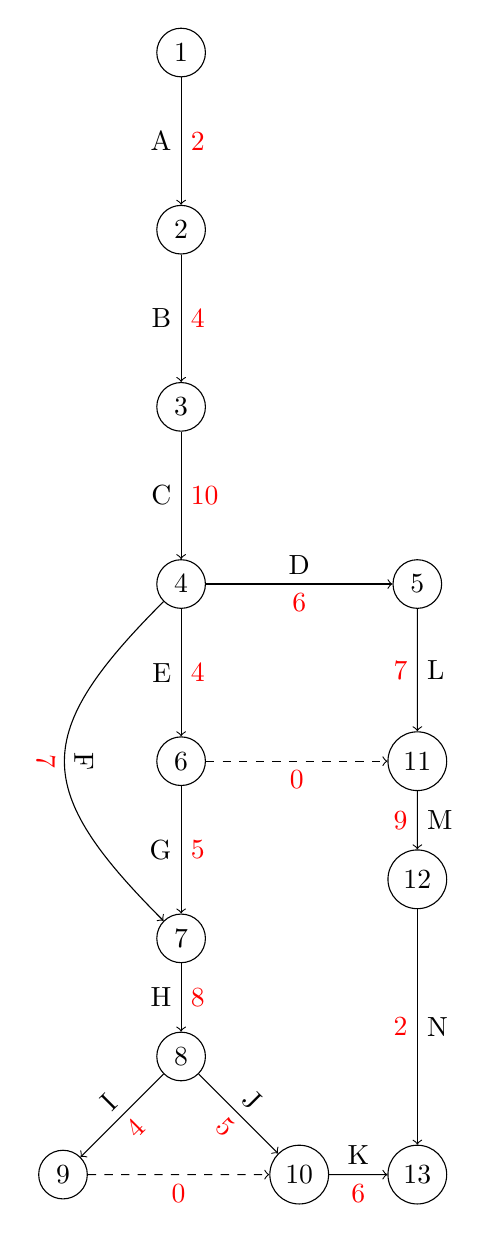
\begin{tikzpicture}[main/.style = {draw, circle}, scale=0.75]] 
            % Nœuds
            \node[main] (1) at (0,13) {1};

            \node[main] (2) at (0,10)  {2};

            \node[main] (3) at (0,7)  {3};

            \node[main] (5) at (4,4)  {5};

            \node[main] (4) at (0,4)  {4};

            \node[main] (6) at (0,1)  {6};

            \node[main] (7) at (0,-2)  {7};

            \node[main] (8) at (0,-4) {8};

            \node[main] (9) at (-2,-6) {9};

            \node[main] (10) at (2,-6) {10};

            \node[main] (11) at (4,1)     {11};

            \node[main] (12) at (4,-1)    {12};

            \node[main] (13) at (4,-6)    {13};


            % Arêtes
            \draw[->] (1) -- node[right] {\textcolor{red}{2}}  node[left] {A} (2);
            \draw[->] (2) -- node[right] {\textcolor{red}{4}}  node[left] { B} (3);
            \draw[->] (3) -- node[right] {\textcolor{red}{10}} node[left] {C} (4);
            \draw[->] (4) -- node[above] {D} node[below] {\textcolor{red}{6}} (5);
            \draw[->] (4) to[bend right=45, looseness=1.5] node[above, sloped] {F} node[below, sloped] {\textcolor{red}{7}} (7);
            \draw[->] (4) -- node[right] {\textcolor{red}{4}} node[left]{E} (6);
            \draw[->] (6) -- node[right] {\textcolor{red}{5}} node[left]{G}   (7);
            \draw[dashed, ->] (6) -- node[below] {\textcolor{red}{0}} (11);
            \draw[->] (7) -- node[right] {\textcolor{red}{8}} node[left]{H}   (8);
            \draw[->] (5) -- node[right] {L} node[left] {\textcolor{red}{7}} (11);
            \draw[->] (11) -- node[right] {M} node[left] {\textcolor{red}{9}} (12);
            \draw[->] (12) -- node[right] {N} node[left] {\textcolor{red}{2}} (13);                   

            \draw[->] (8) -- node[above, sloped] {I} node[below, sloped] {\textcolor{red}{4}} (9);
            \draw[->] (8) -- node[above, sloped] {J} node[below, sloped] {\textcolor{red}{5}} (10);
            \draw[dashed, ->] (9) -- node[above] {} node[below] {\textcolor{red}{0}} (10);
            \draw[->] (10) -- node[above] {K} node[below] {\textcolor{red}{6}} (13);
        \end{tikzpicture}
    }
\end{center}


\begin{table}[H]
    \begin{center}
        \renewcommand{\arraystretch}{2}
        \fontfamily{flr}\selectfont
        \footnotesize
        \begin{tabular}{|l|l|l|l|}
            \hline
            \textbf{Étape} $\boldsymbol{i}$ & $\boldsymbol{j \in B_i}$ 
                                            & $\boldsymbol{ET_j + t_{ji}}$
                                            & $\boldsymbol{ET_i}$   
                                            \\
                                            \hline
                                            \arrayrulecolor{black}
            1 & - & - & 0
            \\
            \hline
            2 & 1 & 0 + 2 & 2  
            \\
            \hline
            3 & 2 & 2 + 4 & 6
            \\ 
            \hline            
            4 & 3 & 6 + 10 & 16 
            \\ 
            \hline            

            5 & 4& 16 + 6 & 22 
            \\ 
            \hline            

            6 & 4 & 16 + 6 & 20 
            \\ 
            \hline           
            7 & \hspace{-1.1em}  
            $\begin{cases}
                4 \\
                6 
            \end{cases}$ 
              & 
              \hspace{-1.1em}
              $\begin{cases}
                  16 + 7 \\ 
                  20 + 5 
              \end{cases}$ 
              & 25
              \\
              \hline            

            8 & 7 & 25 + 8 & 33  
            \\ 

            \hline            

            9 & 8 & 33 + 4 & 37 
            \\ 
            \hline            

            10 & \hspace{-1.1em}
            $\begin{cases}
                8 \\
                9 
            \end{cases}$
               & 
               \hspace{-1.1em}
               $\begin{cases}
                   33 + 4 \\ 
                   37 + 0 
               \end{cases}$ 
               & 38
               \\ 
               \hline  
            11 & \hspace{-1.1em}
            $\begin{cases}
                5 \\
                6 
            \end{cases}$
               & 
               \hspace{-1.1em}
               $\begin{cases}
                   22 + 7 \\ 
                   22 + 0 
               \end{cases}$ 
               & 29
               \\ 

            12 & 11 & 29 + 9 & 38 
            \\ 
            \hline            
            13 & \hspace{-1.1em}
            $\begin{cases}
                10 \\
                12 
            \end{cases}$
               & 
               \hspace{-1.1em}
               $\begin{cases}
                   38 + 6 \\ 
                   38 + 2 
               \end{cases}$ 
               & 44
               \\ 
               \hline
        \end{tabular}
    \end{center}
    \caption {Table des temps de complétions les plus tôt}
\end{table}

Ainsi, de façon générale on a :

\begin{align*}
    \boxed{
        ET_i = \max_{j \in B_i}\Bigl\{ ET_j + t_{ji} \Bigr\}
    }
\end{align*}


Pour \textbf{remplir le tableau des temps de complétions le plus tôt}, 
il faut débuter en haut du tableau en posant 
$ET_{debut} = E_{T_1} = 0$. Ensuite, on trouve le $E_T$ 
pour les tâches $i$ succéssive en applicant la formule récursivement :

% \begin{tikzpicture}[node distance=2.5cm, >=stealth']
%     % Vertices (nodes in circles)
%     \node[circle, draw] (1) {1}; %NODE 1
%     \node[circle, draw] (2) [below of=1] {2}; %NODE 2
%     \node[circle, draw] (C) [below of=2] {3}; %NODE 3
%     \node[circle, draw] (E) [below of=C] {4}; %NODE 4
%     \node[circle, draw] (G) [below of=E] {6}; %NODE 6
%     \node[circle, draw] (F) [below of=E, xshift=-3.5cm] {7}; %NODE7
%     \node[circle, draw] (H) [below of=G] {8}; %NODE 8 
%     \node[circle, draw] (I) [below of=H, node distance=2cm] {9}; %NODE 9
%     \node[circle, draw] (J) [below of=E, xshift=3.5cm] {10}; %NODE 10
%     \node[circle, draw] (L) [below of=J, node distance=2.5cm] {11}; %NODE 11
%     \node[circle, draw] (M) [below right of=I, node distance=2cm] {12}; %NODE 12
%     \node[circle, draw] (N) [below left of=I, node distance=2cm] {13}; %NODE 13
%     \node[circle, draw] (O) [right of=M, node distance=2cm] {14}; %NODE 14
%
%     % 1rrows and labels (arc labels and weights)
%     \draw[->] (1) -- node[left] {A} node[right, color=myr] {2} (2); 
%     \draw[->] (2) -- node[left] {B} node[right, color=myr] {4} (C); 
%     \draw[->] (C) -- node[left] {C} node[right, color=myr] {10} (E);
%     \draw[->] (E) -- node[left] {E} node[right, color=myr] {4} (G);
%     \draw[->] (E) -- node[above, sloped] {F} node[below, sloped, color=myr] {7} (F);
%     \draw[->] (E) -- node[above, sloped] {D} node[below, sloped, color=myr] {6} (J);
%     \draw[->] (G) -- node[left] {G} node[right, color=myr] {5} (H);
%     \draw[->] (H) -- node[left] {H} node[right, color=myr] {8} (I);
%     \draw[->] (I) -- node[above, sloped] {I} node[below,sloped, color=myr] {4} (N);
%     \draw[->] (I) -- node[above, sloped] {J} node[below,sloped, color=myr] {5} (M);
%     \draw[->, dashed] (N) -- node[above, sloped] {} node[below,sloped, color=myr] {5} (M);
%     \draw[->, dashed] (F) -- node[above] {} node[below, sloped, color=myr] {0} (H);
%     \draw[->, dashed] (G) -- node[above, sloped] {} node[below, sloped, color=myr] {0} (L);
%     \draw[->] (M) -- node[above] {K} node[below, color=myr] {6} (O);
%     \draw[->] (J) -- node[left] {M} node[right, color=myr] {9} (L);
%     \draw[->] (L) -- node[left] {N} node[right, color=myr] {2} (O);
% \end{tikzpicture}
\begin{center}
    \scalebox{0.75}{
        \begin{tikzpicture}[main/.style = {draw, circle}, scale=0.75]] 
            % Nœuds
            \node[main] (1) at (0,13) {1};
            \node[right=0.25cm of 1, text=myg] {$0$};

            \node[main] (2) at (0,10)  {2};
            \node[right=0.25cm of 2, text=myg] {$2$};

            \node[main] (3) at (0,7)  {3};
            \node[right=0.25cm of 3, text=myg] {$6$};

            \node[main] (5) at (4,4)  {5};
            \node[right=0.25cm of 5, text=myg] {$22$};

            \node[main] (4) at (0,4)  {4};
            \node[above right=0.25cm of 4, text=myg] {$16$};

            \node[main] (6) at (0,1)  {6};
            \node[above right=0.05cm of 6, text=myg] {$20$};

            \node[main] (7) at (0,-2)  {7};
            \node[right=0.25cm of 7, text=myg] {$25$};

            \node[main] (8) at (0,-4) {8};
            \node[right=0.25cm of 8, text=myg] {$33$};

            \node[main] (9) at (-2,-6) {9};
            \node[below right=0.15cm of 9, text=myg] {$37$};

            \node[main] (10) at (2,-6) {10};
            \node[below=0.25cm of 10, text=myg] {$38$};                 

            \node[main] (11) at (4,1)     {11};
            \node[above right=0.25cm of 11, text=myg] {$29$};

            \node[main] (12) at (4,-1)    {12};
            \node[right=0.25cm of 12, text=myg] {$38$};

            \node[main] (13) at (4,-6)    {13};
            \node[below right=0.15cm of 13, text=myg] {$44$};


            % Arêtes
            \draw[->] (1) -- node[right] {\textcolor{red}{2}}  node[left] {A} (2);
            \draw[->] (2) -- node[right] {\textcolor{red}{4}}  node[left] { B} (3);
            \draw[->] (3) -- node[right] {\textcolor{red}{10}} node[left] {C} (4);
            \draw[->] (4) -- node[above] {D} node[below] {\textcolor{red}{6}} (5);
            \draw[->] (4) to[bend right=45, looseness=1.5] node[above, sloped] {F} node[below, sloped] {\textcolor{red}{7}} (7);
            \draw[->] (4) -- node[right] {\textcolor{red}{4}} node[left]{E} (6);
            \draw[->] (6) -- node[right] {\textcolor{red}{5}} node[left]{G}   (7);
            \draw[dashed, ->] (6) -- node[below] {\textcolor{red}{0}} (11);
            \draw[->] (7) -- node[right] {\textcolor{red}{8}} node[left]{H}   (8);
            \draw[->] (5) -- node[right] {L} node[left] {\textcolor{red}{7}} (11);
            \draw[->] (11) -- node[right] {M} node[left] {\textcolor{red}{9}} (12);
            \draw[->] (12) -- node[right] {N} node[left] {\textcolor{red}{2}} (13);                   

            \draw[->] (8) -- node[above, sloped] {I} node[below, sloped] {\textcolor{red}{4}} (9);
            \draw[->] (8) -- node[above, sloped] {J} node[below, sloped] {\textcolor{red}{5}} (10);
            \draw[dashed, ->] (9) -- node[above] {} node[below] {\textcolor{red}{0}} (10);
            \draw[->] (10) -- node[above] {K} node[below] {\textcolor{red}{6}} (13);
        \end{tikzpicture}
    }
\end{center}



\subsection{Représentation des temps les plus tard}
Les succésseurs de $i$ ont besoin que $i$ se termine 
le plus rapidement possible, pour ne pas retarder 
l'ensemble du projet. Le temps le plus tard auquel $i$ 
peut donc être complété, $LTi$ 
sans affecter le projet dépend du temps de complétion 
le plus petit d'un successeur de $i$,
\begin{align*}
    \boxed{
        LT_i = \max_{j \in P_i}\Bigl\{ LT_j - t_{ji} \Bigr\}
    }
\end{align*}

\begin{table}[H]
    \begin{center}
        \renewcommand{\arraystretch}{2}
        \fontfamily{flr}\selectfont
        \footnotesize
        \begin{tabular}{|l|l|l|l|}
            \hline
            \textbf{Étape} $\boldsymbol{i}$ & $\boldsymbol{j \in P_i}$ 
                                            & $\boldsymbol{LT_j + t_{ji}}$
                                            & $\boldsymbol{LT_i}$   
                                            \\
                                            \hline
                                            \arrayrulecolor{black}
            13 & - & - & 44
            \\
            \hline
            12 & 13 & 44 - 2 & 42  
            \\
            \hline
            11 & 12 & 42 - 9 & 33
            \\ 
            \hline            
            10 & 13 & 44 - 6 & 38 
            \\ 
            \hline            

            9  & 10 & 38 - 0 & 38
            \\ 
            \hline            

            8 & \hspace{-1.1em}  
            $\begin{cases}
                10 \\
                9
            \end{cases}$ 
              & 
              \hspace{-1.1em}
              $\begin{cases}
                  38 - 5 \\ 
                  38 - 4 
              \end{cases}$ 
              & 33 

              \\ 
              \hline

            7 & 8 & 33 - 8 & 25 
            \\
            \hline

            6 & \hspace{-1.1em}  
            $\begin{cases}
                11 \\
                7
            \end{cases}$ 
              & 
              \hspace{-1.1em}
              $\begin{cases}
                  33 - 0 \\ 
                  25 - 5 
              \end{cases}$ 
              & 20 
              \\
              \hline            

            5 & 11 & 37 - 7 & 26 
            \\ 
            \hline           
            4 & \hspace{-1.1em}  
            $\begin{cases}
                7 \\
                6 \\  
                5
            \end{cases}$ 
              & \hspace{-.2em} 
              \hspace{-1.1em}
              $\begin{cases}
                  25 - 7 \\ 
                  20 - 4 \\ 
                  26 - 6 \\
              \end{cases}$ 
              & 16
              \\
              \hline            

            3 & 4 & 16 - 10 & 6  
            \\ 

            \hline            

            2 & 3 & 6 - 4 & 2 
            \\ 
            \hline           
            1 & 2 & 2 - 2 & 0 
            \\ 
            \hline
        \end{tabular}
    \end{center}
    \caption {Projet de construction d'une maison}
\end{table}

\begin{center}
    \scalebox{0.75}{
        \begin{tikzpicture}[main/.style = {draw, circle}, scale=0.75]] 
            % Nœuds
            \node[main] (1) at (0,13) {1};
            \node[right=0.25cm of 1, text=myg] {$0$};
            \node[left=0.25cm of 1, text=myb] {$0$};

            \node[main] (2) at (0,10)  {2};
            \node[right=0.25cm of 2, text=myg] {$2$};
            \node[left=0.25cm of 2, text=myb] {$2$};

            \node[main] (3) at (0,7)  {3};
            \node[right=0.25cm of 3, text=myg] {$6$};
            \node[left=0.25cm of 3, text=myb] {$6$};

            \node[main] (5) at (4,4)  {5};
            \node[right=0.25cm of 5, text=myg] {$22$};
            \node[above left=0.25cm of 5, text=myb] {$26$};

            \node[main] (4) at (0,4)  {4};
            \node[above right=0.25cm of 4, text=myg] {$16$};
            \node[above left=0.25cm of 4, text=myb] {$16$};                 

            \node[main] (6) at (0,1)  {6};
            \node[above right=0.05cm of 6, text=myg] {$20$};
            \node[above left=0.05cm of 6, text=myb] {$20$};

            \node[main] (7) at (0,-2)  {7};
            \node[right=0.25cm of 7, text=myg] {$25$};
            \node[left=0.25cm of 7, text=myb] {$25$};

            \node[main] (8) at (0,-4) {8};
            \node[right=0.25cm of 8, text=myg] {$33$};
            \node[left=0.25cm of 8, text=myb] {$33$};

            \node[main] (9) at (-2,-6) {9};
            \node[below right=0.15cm of 9, text=myg] {$37$};
            \node[below left=0.15cm of 9, text=myb] {$38$};

            \node[main] (10) at (2,-6) {10};
            \node[below=0.25cm of 10, text=myg] {$38$};                 
            \node[below left=0.5cm of 10, text=myb] {$38$};

            \node[main] (11) at (4,1)     {11};
            \node[above right=0.25cm of 11, text=myg] {$29$};
            \node[above left=0.25cm of 11, text=myb] {$33$};

            \node[main] (12) at (4,-1)    {12};
            \node[right=0.25cm of 12, text=myg] {$38$};
            \node[left=0.25cm of 12, text=myb] {$42$};

            \node[main] (13) at (4,-6)    {13};
            \node[below right=0.15cm of 13, text=myg] {$44$};
            \node[below left=0.15cm of 13, text=myb] {$44$};


            % Arêtes
            \draw[->] (1) -- node[right] {\textcolor{red}{2}}  node[left] {A} (2);
            \draw[->] (2) -- node[right] {\textcolor{red}{4}}  node[left] { B} (3);
            \draw[->] (3) -- node[right] {\textcolor{red}{10}} node[left] {C} (4);
            \draw[->] (4) -- node[above] {D} node[below] {\textcolor{red}{6}} (5);
            \draw[->] (4) to[bend right=45, looseness=1.5] node[above, sloped] {F} node[below, sloped] {\textcolor{red}{7}} (7);
            \draw[->] (4) -- node[right] {\textcolor{red}{4}} node[left]{E} (6);
            \draw[->] (6) -- node[right] {\textcolor{red}{5}} node[left]{G}   (7);
            \draw[dashed, ->] (6) -- node[below] {\textcolor{red}{0}} (11);
            \draw[->] (7) -- node[right] {\textcolor{red}{8}} node[left]{H}   (8);
            \draw[->] (5) -- node[right] {L} node[left] {\textcolor{red}{7}} (11);
            \draw[->] (11) -- node[right] {M} node[left] {\textcolor{red}{9}} (12);
            \draw[->] (12) -- node[right] {N} node[left] {\textcolor{red}{2}} (13);                   

            \draw[->] (8) -- node[above, sloped] {I} node[below, sloped] {\textcolor{red}{4}} (9);
            \draw[->] (8) -- node[above, sloped] {J} node[below, sloped] {\textcolor{red}{5}} (10);
            \draw[dashed, ->] (9) -- node[above] {} node[below] {\textcolor{red}{0}} (10);
            \draw[->] (10) -- node[above] {K} node[below] {\textcolor{red}{6}} (13);
        \end{tikzpicture}
    }
\end{center}
L'écart pour la tâche associée à l'arrête $ij$ 
est le délai maximal permettant de compléter 
la tâchge sans retarder l'achèvement du projet à 
son temps le plus tôt. 
\begin{align*}
    \boxed{
        EC_{ij} = LT_j - (ET_i + t_{ij}) 
    }
\end{align*}


\begin{tikzpicture}[>=stealth']

    % Nodes (i and j)

    \node[circle, draw, minimum size=8pt, inner sep=1pt] (i) at (-2.5, -0.15) {$i$};
    \node[circle, draw, minimum size=8pt, inner sep=1pt] (j) at (1.5, -0.15) {$j$};

    % Arrow between nodes with label
    \draw[->] (i) -- node[above] {$t_{ij}$} (j);

    % Timeline representation
    \draw[->] (-3, -2) -- (3, -2) node[right] {$t$};
    \draw (-2.5, -2) -- (-2.5, -1.8) node[below, yshift=-.5cm] {$ET_i$};
    \draw (.25, -2) -- (.25, -1.8) node[below, yshift=-.5cm] {$ET_i + t_{ij}$};
    \draw (1.5, -2) -- (1.5, -1.8) node[below, yshift=-.5cm] {$LT_j$};

    % Arrows for ECij
    \draw[<->] (.25, -1.4) -- node[above] {$EC_{ij}$} (1.5, -1.4);

\end{tikzpicture}

\begin{center}
\begin{tikzpicture}[>=stealth']

    % Nodes
    \node[circle, draw, minimum size=8pt, inner sep=1pt] (node4) {4};
    \node[circle, draw, minimum size=8pt, inner sep=1pt, below=1.5cm of node4] (node6) {6};
    \node[circle, draw, minimum size=8pt, inner sep=1pt, below=1.5cm of node6] (node7) {7};

    % Arrows and labels
    \draw[->] (node4) -- node[right] {} (node6);
    \draw[->] (node6) -- node[right] {} (node7);

    % Curved arc from node4 to node7
    \draw[->, bend right=45] (node4) to node[right] {F} node[left, color=red] {7} (node7);

    % Text labels for times
    \node[above left=-0.1cm of node4, color=myb] {16};
    \node[above right=-0.1cm of node4, color=myg] {16};

    \node[below left=-0.1cm of node7, color=myb] {25};
    \node[below right=-0.1cm of node7, color=myg] {25};
\end{tikzpicture}
\end{center}

             \begin{table}[H]
              \begin{center}
   \begin{tabular}{|c|c|}
        \hline
        \textbf{Tâche $(i, j)$} & \textbf{Écart $LT_j - (ET_i + t_{ij})$} \\
        \hline
        (1, 2) & $2 - (0 + 2) = 0$ \\
        (2, 3) & $6 - (2 + 4) = 0$ \\
        (3, 4) & $16 - (6 + 10) = 0$ \\
        (4, 5) & $26 - (16 + 6) = 4$ \\
        (4, 6) & $20 - (16 + 4) = 0$ \\
        (4, 7) & $25 - (16 + 7) = 2$ \\
        (6, 7) & $25 - (20 + 5) = 0$ \\
        (7, 8) & $33 - (25 + 8) = 0$ \\
        (8, 9) & $38 - (33 + 4) = 1$ \\
        (8, 10) & $38 - (33 + 5) = 0$ \\
        (10, 13) & $44 - (38 + 6) = 0$ \\
        (5, 11) & $33 - (22 + 7) = 4$ \\
        (11, 12) & $42 - (29 + 9) = 4$ \\
        (12, 13) & $44 - (38 + 2) = 4$ \\
        (6, 11) & $33 - (20 + 0) = 13$ \\
        (9, 10) & $38 - (37 + 0) = 1$ \\
        \hline
    \end{tabular}                
\end{center}
\caption{Écart $LT_j - (ET_i + t_{ij})$ pour chaque tâche $(i, j)$}
            \end{table}



            \begin{center}
            \scalebox{0.75}{
                \begin{tikzpicture}[main/.style = {draw, circle}, scale=0.75]] 
                  % Nœuds
                  \node[main] (1) at (0,13) {1};
                  \node[right=0.25cm of 1, text=myg] {$0$};
                  \node[left=0.25cm of 1, text=myb] {$0$};
                  
                  \node[main] (2) at (0,10)  {2};
                  \node[right=0.25cm of 2, text=myg] {$2$};
                  \node[left=0.25cm of 2, text=myb] {$2$};
                  
                  \node[main] (3) at (0,7)  {3};
                  \node[right=0.25cm of 3, text=myg] {$6$};
                  \node[left=0.25cm of 3, text=myb] {$6$};
                  
                  \node[main] (5) at (4,4)  {5};
                  \node[right=0.25cm of 5, text=myg] {$22$};
                  \node[above left=0.25cm of 5, text=myb] {$26$};
                  
                  \node[main] (4) at (0,4)  {4};
                  \node[above right=0.25cm of 4, text=myg] {$16$};
                   \node[above left=0.25cm of 4, text=myb] {$16$};                 

                  \node[main] (6) at (0,1)  {6};
                  \node[above right=0.05cm of 6, text=myg] {$20$};
                  \node[above left=0.05cm of 6, text=myb] {$20$};
                  
                  \node[main] (7) at (0,-2)  {7};
                  \node[right=0.25cm of 7, text=myg] {$25$};
                  \node[left=0.25cm of 7, text=myb] {$25$};
                  
                  \node[main] (8) at (0,-4) {8};
                  \node[right=0.25cm of 8, text=myg] {$33$};
                  \node[left=0.25cm of 8, text=myb] {$33$};

                  \node[main] (9) at (-2,-6) {9};
                  \node[below right=0.15cm of 9, text=myg] {$37$};
                  \node[below left=0.15cm of 9, text=myb] {$38$};

                  \node[main] (10) at (2,-6) {10};
                  \node[below=0.25cm of 10, text=myg] {$38$};                 
                  \node[below left=0.5cm of 10, text=myb] {$38$};

                  \node[main] (11) at (4,1)     {11};
                  \node[above right=0.25cm of 11, text=myg] {$29$};
                  \node[above left=0.25cm of 11, text=myb] {$33$};

                  \node[main] (12) at (4,-1)    {12};
                  \node[right=0.25cm of 12, text=myg] {$38$};
                  \node[left=0.25cm of 12, text=myb] {$42$};

                  \node[main] (13) at (4,-6)    {13};
                  \node[below right=0.15cm of 13, text=myg] {$44$};
                  \node[below left=0.15cm of 13, text=myb] {$44$};


                  % Arêtes
                    \draw[->] (1) -- node[right] {\textcolor{red}{2}}  node[left] {\textcolor{myp}{0}  A} (2);
                    \draw[->] (2) -- node[right] {\textcolor{red}{4}}  node[left] {\textcolor{myp}{0} B} (3);
                    \draw[->] (3) -- node[right] {\textcolor{red}{10}} node[left] {\textcolor{myp}{0} C} (4);
                    \draw[->] (4) -- node[above] {\textcolor{myp}{0} D} node[below] {\textcolor{red}{6}} (5);
                    \draw[->] (4) to[bend right=45, looseness=1.5] node[above, sloped] {\textcolor{myp}{2} F} node[below, sloped] {\textcolor{red}{7}} (7);
                    \draw[->] (4) -- node[right] {\textcolor{red}{4}} node[left]{\textcolor{myp}{0} E} (6);
                    \draw[->] (6) -- node[right] {\textcolor{red}{5}} node[left]{\textcolor{myp}{0} G}   (7);
                    \draw[dashed, ->] (6) -- node[below] {\textcolor{red}{0}} (11);
                    \draw[->] (7) -- node[right] {\textcolor{red}{8}} node[left]{\textcolor{myp}{0} H}   (8);
                    \draw[->] (5) -- node[right] {\textcolor{myp}{4} L} node[left] {\textcolor{red}{7}} (11);
                    \draw[->] (11) -- node[right] {\textcolor{myp}{4} M} node[left] {\textcolor{red}{9}} (12);
                     \draw[->] (12) -- node[right] {\textcolor{myp}{4} N} node[left] {\textcolor{red}{2}} (13);                   

                    \draw[->] (8) -- node[above, sloped] {\textcolor{myp}{1} I} node[below, sloped] {\textcolor{red}{4}} (9);
                    \draw[->] (8) -- node[above, sloped] {\textcolor{myp}{0} J} node[below, sloped] {\textcolor{red}{5}} (10);
                    \draw[dashed, ->] (9) -- node[above] {\textcolor{myp}{1}} node[below] {\textcolor{red}{0}} (10);
                    \draw[->] (10) -- node[above] {\textcolor{myp}{0} K} node[below] {\textcolor{red}{6}} (13);
                \end{tikzpicture}
            }
            \end{center}
            \vspace{-2em}
    \subsection{Chemin critique}
    Le chemin critique est un 
    chemin du sommet début au 
    sommet fin le long duquel 
    toutes les tâches (arcs) ont un 
    écart nul.

\begin{center}
\scalebox{0.70}{
    \begin{tikzpicture}[main/.style = {draw, circle}, scale=0.65] 
      % Nodes
      \node[main] (1) at (0,13) {1};
      \node[right=0.25cm of 1, text=myg] {$0$};
      \node[left=0.25cm of 1, text=myb] {$0$};
      
      \node[main] (2) at (0,10)  {2};
      \node[right=0.25cm of 2, text=myg] {$2$};
      \node[left=0.25cm of 2, text=myb] {$2$};
      
      \node[main] (3) at (0,7)  {3};
      \node[right=0.25cm of 3, text=myg] {$6$};
      \node[left=0.25cm of 3, text=myb] {$6$};
      
      \node[main] (4) at (0,4)  {4};
      \node[above right=0.25cm of 4, text=myg] {$16$};
      \node[above left=0.25cm of 4, text=myb] {$16$};                 

      \node[main] (6) at (0,1)  {6};
      \node[above right=0.05cm of 6, text=myg] {$20$};
      \node[above left=0.05cm of 6, text=myb] {$20$};
      
      \node[main] (7) at (0,-2)  {7};
      \node[right=0.25cm of 7, text=myg] {$25$};
      \node[left=0.25cm of 7, text=myb] {$25$};
      
      \node[main] (8) at (0,-4) {8};
      \node[right=0.25cm of 8, text=myg] {$33$};
      \node[left=0.25cm of 8, text=myb] {$33$};

      \node[main] (10) at (2,-6) {10};
      \node[below=0.25cm of 10, text=myg] {$38$};                 
      \node[below left=0.5cm of 10, text=myb] {$38$};

      \node[main] (13) at (4,-6)    {13};
      \node[below right=0.15cm of 13, text=myg] {$44$};
      \node[below left=0.15cm of 13, text=myb] {$44$};


      % Edges (critical path only)
      \draw[->, myr, thick] (1) -- node[right] {\textcolor{red}{2}}  node[left] {\textcolor{myp}{0} A} (2);
      \draw[->, myr, thick] (2) -- node[right] {\textcolor{red}{4}}  node[left] {\textcolor{myp}{0} B} (3);
      \draw[->, myr, thick] (3) -- node[right] {\textcolor{red}{10}} node[left] {\textcolor{myp}{0} C} (4);
      \draw[->, myr, thick] (4) -- node[right] {\textcolor{red}{4}} node[left]{\textcolor{myp}{0} E} (6);
      \draw[->, myr, thick] (6) -- node[right] {\textcolor{red}{5}} node[left]{\textcolor{myp}{0} G} (7);
      \draw[->, myr, thick] (7) -- node[right] {\textcolor{red}{8}} node[left]{\textcolor{myp}{0} H} (8);
      \draw[->, myr, thick] (8) -- node[above, sloped] {\textcolor{myp}{0} J} node[below, sloped] {\textcolor{red}{5}} (10);
      \draw[->, myr, thick] (10) -- node[above] {\textcolor{myp}{0} K} node[below] {\textcolor{red}{6}} (13);
    \end{tikzpicture}
}
\end{center}

    Les tâches d’écart nul sont 
    critiques car tout délai dans leur 
    réalisation \textbf{entraîne un retard }   
    dans l’achèvement du projet au 
    temps le plus tôt.

\blankpage
    \chapter{Optimisation de Graphes et Réseaux 4}
\section{Abre partiel de poids minimal}




\subsection{Théorie}
\begin{itemize}
    \item[$\rhd$] \textbf{Définitions et rappels} :
    \begin{itemize}
        \item[$\blacktriangleright$ ] Un \textbf{graphe connexe} est un graphe dans lequel il existe une chaîne reliant chaque paire de sommets distincts.
\end{itemize}
\end{itemize}


\noindent \begin{minipage}{.25\textwidth}
            \begin{center}
                \scalebox{0.75}{
            \begin{tikzpicture}[node distance=2cm, main/.style = {draw, circle}] 
            % Premier graphe
                \node[main] (1) {1}; 
                \node[main] (3) [below right=1cm and 2cm of 1] {3}; 
                \node[main] (2) [below left=1cm and 2cm of 3] {2};
                \draw (1) -- node[above] {c} (3);
                \draw (1) to[bend right] node[left] {a} (2);
                \draw (1) to[bend left] node[right] {b} (2);
                \draw (2) -- node[below] {d} (3);
           \end{tikzpicture}
       }
           \label{$G$}
           \\
           \textbf{Connexe}  
            \end{center}
            \end{minipage}%
            \begin{minipage}{.25\textwidth}
          \begin{center}
            \scalebox{0.75}{
            \begin{tikzpicture}[node distance=2cm, main/.style = {draw, circle}] 
            % Premier graphe
                \node[main] (1) {1}; 
                \node[main] (3) [below right=1cm and 2cm of 1] {3}; 
                \node[main] (2) [below left=1cm and 2cm of 3] {2};
                \draw (1) -- node[above] {c} (3);
           \end{tikzpicture}
       }
           \label{Arbre partiel}
           \\
           \textbf{Non connexe}  
            \end{center}
            \end{minipage}

\begin{itemize}
    \item [\phantom{$\rhd$} ] \phantom{Définitions et rappels} 
        \begin{itemize}
        \item[$\blacktriangleright$ ] Un \textbf{sous-graphe} \( G' \) d'un graphe \( G \) contient un sous-ensemble des sommets et arêtes de \( G \).
        \end{itemize} 
\end{itemize}

\vspace{1em}
\noindent
                \begin{minipage}{.25\textwidth}
                \begin{center}
                    \scalebox{0.75}{
                \begin{tikzpicture}[node distance=2cm, main/.style = {draw, circle}] 
                % Premier graphe
                    \node[main] (1) {1}; 
                    \node[main] (3) [below right=1cm and 2cm of 1] {3}; 
                    \node[main] (2) [below left=1cm and 2cm of 3] {2};
                    \draw (1) -- node[above] {c} (3);
                    \draw (1) to[bend right] node[left] {a} (2);
                    \draw (1) to[bend left] node[right] {b} (2);
                    \draw (2) -- node[below] {d} (3);
               \end{tikzpicture}
           }
               \label{$G$}
               \\
               \textbf{Graphe G}  
                \end{center}
                \end{minipage}%
                \begin{minipage}{.25\textwidth}
              \begin{center}
                \scalebox{0.75}{
                \begin{tikzpicture}[node distance=2cm, main/.style = {draw, circle}] 
                % Premier graphe
                    \node[main] (1) {1}; 
                    \node[main] (2) [below left=1cm and 2cm of 3] {2};

                    \node[] (3) [below right=1cm and 2cm of 1] {\phantom{3}}; 

                    \draw (1) to[bend right] node[left] {a} (2);
               \end{tikzpicture}
           }
               \label{Arbre partiel}
               \\
               \textbf{Sous-graphe $\boldsymbol{G^{\prime}}$  }  
                \end{center}
                \end{minipage}

\begin{itemize}
    \item [\phantom{$\rhd$} ] \phantom{Définitions et rappels} 
        \begin{itemize}
        \item[$\blacktriangleright$ ] Un \textbf{graphe partiel} est un sous-graphe qui contient tous les sommets de \( G \).
        \end{itemize}
\end{itemize}


\vspace{1em}
\noindent
                \begin{minipage}{.25\textwidth}
                \begin{center}
                    \scalebox{0.75}{
                \begin{tikzpicture}[node distance=2cm, main/.style = {draw, circle}] 
                % Premier graphe
                    \node[main] (1) {1}; 
                    \node[main] (3) [below right=1cm and 2cm of 1] {3}; 
                    \node[main] (2) [below left=1cm and 2cm of 3] {2};
                    \draw (1) -- node[above] {c} (3);
                    \draw (1) to[bend right] node[left] {a} (2);
                    \draw (1) to[bend left] node[right] {b} (2);
                    \draw (2) -- node[below] {d} (3);
               \end{tikzpicture}
           }
               \label{$G$}
               \\
               \textbf{Graphe G}  
                \end{center}
                \end{minipage}%
                \begin{minipage}{.25\textwidth}
              \begin{center}
                \scalebox{0.75}{
                \begin{tikzpicture}[node distance=2cm, main/.style = {draw, circle}] 
                % Premier graphe
                    \node[main] (1) {1}; 
                    \node[main] (3) [below right=1cm and 2cm of 1] {3}; 
                    \node[main] (2) [below left=1cm and 2cm of 3] {2};

                    \draw (1) to[bend right] node[left] {a} (2);
               \end{tikzpicture}
           }
               \label{Arbre partiel}
               \\
               \textbf{Graphe partiel $\boldsymbol{G^{\prime}}$  }  
                \end{center}
                \end{minipage}

\begin{itemize}
    \item [\phantom{$\rhd$} ] \phantom{Définitions et rappels} 
    \begin{itemize}
        \item[$\blacktriangleright$ ] Un \textbf{arbre} est un graphe connexe sans cycle. Il a exactement \( n-1 \) arêtes pour \( n \) sommets.
        \item[$\blacktriangleright$ ] Un \textbf{arbre partiel} ou arbre \textbf{de recouvrement} 
            est un sous-graphe connexe et sans cycle contenant tous les sommets du graphe.
            Autrement dit, c'est un arbre qui se trouve à être un également un graphe partiel. 
    \end{itemize}


                \begin{minipage}{.25\textwidth}
                \begin{center}
                    \scalebox{0.75}{
                \begin{tikzpicture}[node distance=2cm, main/.style = {draw, circle}] 
                % Premier graphe
                    \node[main] (1) {1}; 
                    \node[main] (3) [below right=1cm and 2cm of 1] {3}; 
                    \node[main] (2) [below left=1cm and 2cm of 3] {2};
                    \draw (1) -- node[above] {c} (3);
                    \draw (1) to[bend right] node[left] {a} (2);
                    \draw (1) to[bend left] node[right] {b} (2);
                    \draw (2) -- node[below] {d} (3);
               \end{tikzpicture}
           }
               \label{$G$}
               \\
               \textbf{Graphe G}  
                \end{center}
                \end{minipage}%
                \begin{minipage}{.25\textwidth}
              \begin{center}
                \scalebox{0.75}{
                \begin{tikzpicture}[node distance=2cm, main/.style = {draw, circle}] 
                % Premier graphe
                    \node[main] (1) {1}; 
                    \node[main] (3) [below right=1cm and 2cm of 1] {3}; 
                    \node[main] (2) [below left=1cm and 2cm of 3] {2};


                    \draw (2) -- node[below] {d} (3);
                    \draw (1) -- node[above] {c} (3);
               \end{tikzpicture}
           }
               \label{Arbre partiel}
               \\
               \textbf{Arbre partiel $\boldsymbol{G^{\prime}}$  }  
                \end{center}
                \end{minipage}


    \subsection{Analyse des arbre partiels}
    \item[$\rhd$] \textbf{Arbre partiel de poids minimal} :
    \begin{itemize}
        \item [$\blacktriangleright$ ]  Un \textbf{arbre partiel de poids minimal} est un arbre de recouvrement dont la somme des poids des arêtes est minimale.
        \item [$\blacktriangleright$ ] Problème concret : Minimiser le coût de connexion des habitations par des lignes électriques en identifiant un arbre partiel de poids minimal.
    \end{itemize}

                \begin{center}
                        \begin{tikzpicture}[main/.style = {draw, circle}] 
                        % Définition des nœuds
                        \node[main] (1) at (0,0) {}; 
                        \node[main] (2) at (2,1) {}; 
                        \node[main] (3) at (1,3) {};
                        \node[main] (4) at (-1,3) {};
                        \node[main] (5) at (-2,1) {};
                        
                        % Définition des arêtes
                        \draw[myg, thick] (1) -- node[below, sloped] {10} (2);
                        \draw[myg, thick] (2) -- node[sloped, above] {40} (3);

                        \draw[myg, thick] (3) -- node[above] {25} (4);
                        \draw[] (4) -- node[sloped, above] {100} (5);

                        \draw[myg, thick] (5) -- node[sloped, below] {25} (3);

                            \draw[] (5) -- node[below, sloped] {50} (1);
                                    \draw[] (1) -- node[sloped, below] {200} (3);
                        \end{tikzpicture}
                \end{center}
                \begin{center}
                \textbf{Poids total}   : $25 + 25 + 40 + 10 = 100$
                \end{center}

\end{itemize}
    \subsection{Principe de l'algorithme de Kruskal}
    \begin{itemize}
        \item [$\blacktriangleright$ ]  Algorithme dit vorace ou \textit{greedy}   
            pour trouver un arbre partiel de poids minimal.
    \end{itemize}

    \begin{center}
     \scalebox{0.75}{
                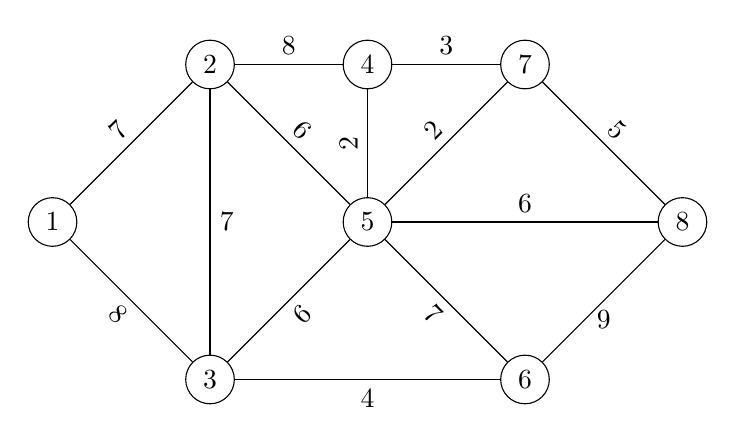
\begin{tikzpicture}[main/.style = {draw, circle}] 
                % Nœuds
                \node[main] (1) at (-1,0) {1};
                \node[main] (2) at (1,2) {2};
                \node[main] (3) at (1,-2) {3};
                \node[main] (4) at (3,2) {4};
                \node[main] (5) at (3,0) {5};
                \node[main] (6) at (5,-2) {6};
                \node[main] (7) at (5,2) {7};
                \node[main] (8) at (7,0) {8};

                % Arêtes
                \draw[] (1) -- node[sloped, above, ] {7} (2);
                \draw[] (1) -- node[sloped, below, ] {8} (3);
                \draw[] (2) -- node[above, ] {8} (4);
                \draw[] (2) -- node[right, ] {7} (3);
                \draw[] (2) -- node[sloped, above, ] {6} (5);
                \draw[] (3) -- node[sloped, below, ] {6} (5);
                \draw[] (3) -- node[below, ] {4} (6);
                \draw[] (4) -- node[above, ] {3} (7);
                \draw[] (5) -- node[sloped, above, ] {2} (4);
                \draw[] (5) -- node[sloped, below, ] {7} (6);
                \draw[] (5) -- node[sloped, above, ] {2} (7);
                \draw[] (5) -- node[sloped, above, ] {6} (8);
                \draw[] (6) -- node[below, ] {9} (8);
                \draw[] (7) -- node[sloped, above, ] {5} (8);
                \end{tikzpicture}
        }
    \end{center}
        \begin{enumerate}
            \item Initialiser l'ensemble \(\Omega = \emptyset\) et un compteur \(k = 0\).
            \item Choisir l'arête de plus petit poids dans \(E \setminus \Omega\) qui ne forme pas de cycle avec les arêtes de \(\Omega\).
            \item Ajouter cette arête à \(\Omega\) et incrémenter \(k\).
            \item Répéter jusqu'à obtenir \(n-1\) arêtes.
        \end{enumerate}

                \begin{align*}
                    (4, 5) & \quad \textcolor{myg}{k = 1}   \\ 
                    (5, 7) &\quad  \textcolor{myg}{k = 2}   \\ 
                    (4, 7) &  \quad \text{ignoré }\\ 
                    (3, 6) & \quad \textcolor{myg}{k = 3}  \\ 
                    (7, 8) & \quad \textcolor{myg}{k = 4}  \\ 
                    (2, 5) & \quad \textcolor{myg}{k = 5}  \\ 
                    (3, 5) & \quad \textcolor{myg}{k = 6}  \\ 
                    (5, 8) & \quad \text{ignoré} \\ 
                    (1, 2) & \quad \textcolor{myg}{k = 7}  \\ 
                    (2, 3) & \quad \text{ignoré} \\ 
                    (5, 6) & \quad \text{ignoré}       \\ 
                    (1, 3) & \quad \text{ignoré} \\
                    (2, 4) & \quad \text{ignoré} \\ 
                    (6, 8) & \quad \text{ignoré}
                \end{align*}

    \begin{center}
     \scalebox{0.75}{
                \begin{tikzpicture}[main/.style = {draw, circle}] 
                % Nœuds
                \node[main] (1) at (-1,0) {1};
                \node[main] (2) at (1,2) {2};
                \node[main] (3) at (1,-2) {3};
                \node[main] (4) at (3,2) {4};
                \node[main] (5) at (3,0) {5};
                \node[main] (6) at (5,-2) {6};
                \node[main] (7) at (5,2) {7};
                \node[main] (8) at (7,0) {8};

                % Arêtes
                \draw[myg, thick] (1) -- node[sloped, above, ] {7} (2);
                \draw[] (1) -- node[sloped, below, ] {8} (3);
                \draw[] (2) -- node[above, ] {8} (4);
                \draw[] (2) -- node[right, ] {7} (3);
                \draw[myg, thick] (2) -- node[sloped, above, ] {6} (5);
                \draw[myg, thick] (3) -- node[sloped, below, ] {6} (5);
                \draw[myg, thick] (3) -- node[below, ] {4} (6);
                \draw[] (4) -- node[above, ] {3} (7);
                \draw[myg, thick] (5) -- node[sloped, above, ] {2} (4);
                \draw[] (5) -- node[sloped, below, ] {7} (6);
                \draw[myg, thick] (5) -- node[sloped, above, ] {2} (7);
                \draw[] (5) -- node[sloped, above, ] {6} (8);
                \draw[] (6) -- node[below, ] {9} (8);
                \draw[myg, thick] (7) -- node[sloped, above, ] {5} (8);
                \end{tikzpicture}
        }
    \end{center}

\newpage

\chapter{Programmation dynamique déterministe}
\section{Introduction}

\begin{itemize}
    \item [$\rhd$ ]\textbf{Contexte}   
    \begin{itemize}
        \item [$\blacktriangleright$ ] S'applique aux problèmes où la 
            solution correspond à \textbf{une suite de décision}. 
    \end{itemize}
    \item [$\rhd$ ] \textbf{Objectif}  
        \begin{itemize}
            \item [$\blacktriangleright$ ] Réduire le problème original en sous-problèmes.
            \item [$\blacktriangleright$ ] Chaque sous-problème doit être plus simple à résoudre.  
        \end{itemize}
    \item [$\rhd$ ] \textbf{Application }   
        \begin{itemize}
            \item [$\blacktriangleright$ ] Exploiter la solution des sous-problèmes les plus 
                simples afin de produire la solution optimale des sous-problèmes complexes. 
            \item [$\blacktriangleright$ ] Résoudre ainsi les sous-problèmes complexe pour obtenir  
                la \textbf{solution optimale du problème original}  
        \end{itemize}
\end{itemize}

\begin{tikzpicture}[scale=0.85, 
    ->,>=stealth',shorten >=1pt,auto,node distance=2cm,
    thick,main node/.style={circle,draw}
]

% Noeuds
\node[main node] (1) {1};
\node[main node] (3) [right of=1] {3};

\node[main node] (2) [above of=3] {2};
\node[main node] (4) [below of=3] {4};
\node[main node] (5) [right of=2] {5};
\node[main node] (6) [right of=3] {6};
\node[main node] (7) [right of=4] {7};
\node[main node] (8) [above right of=6] {8};
\node[main node] (9) [below right of=6] {9};
\node[main node] (10) [right=2.5cm of 6] {10};

% Arcs
\path[every node/.style={font=\sffamily\small}]

    (1) edge node[pos=0.2, above] {2} (2)
        edge node[pos=0.2, above] {4} (3)
        edge node[pos=0.2, above] {3} (4)
    (2) edge node[pos=0.2, above] {7} (5)
        edge node[pos=0.2, above] {4} (6)
        edge node[pos=0.2, above] {6} (7)
    (3) edge node[pos=0.2, above] {3} (5)
        edge node[pos=0.2, above] {2} (6)
        edge node[pos=0.2, above] {4} (7)
    (4) edge node[pos=0.2, above] {4} (5)
        edge node[pos=0.2, above] {1} (6)
        edge node[pos=0.2, above] {5} (7)
    (5) edge node[pos=0.2, above] {1} (8)
        edge node[pos=0.2, above] {4} (9)
    (6) edge node[pos=0.2, above] {6} (8)
        edge node[pos=0.2, above] {3} (9)
    (7) edge node[pos=0.2, above] {3} (8)
        edge node[pos=0.2, above] {3} (9)
    (8) edge node[pos=0.2, above] {3} (10)
    (9) edge node[pos=0.2, above] {4} (10);
\end{tikzpicture}

\section{Exemple chemin le plus court}
L'algorithme de Dijkstra permettrait de trouver le chemin le plus court. 
Cependant, la structure du graphe se prette bien à l'utilisation 
d'une approche de \textbf{programmation dynamique}  




\begin{tikzpicture}[scale=0.85, 
    ->,>=stealth',shorten >=1pt,auto,node distance=2cm,
    thick,main node/.style={circle,draw}
]

% Colonnes
\draw[dashed] (1.05,-4) -- (1.05,4);
\draw[dashed] (3.05,-4) -- (3.05,4);
\draw[dashed] (5.05,-4) -- (5.05,4);
\draw[dashed] (7.25,-4) -- (7.25,4);

% Numéros de colonnes
\node[draw=green, thick, text=black] at (0,4.5) {1};
\node[draw=green, thick, text=black] at (1.75,4.5) {2};
\node[draw=green, thick, text=black] at (3.75,4.5) {3};
\node[draw=green, thick, text=black] at (6,4.5) {4};
\node[draw=green, thick, text=black] at (7.75,4.5) {5};

% Noeuds
\node[main node] (1) at (0,0) {1};
\node[main node] (2) at (2,2) {2};
\node[main node] (3) at (2,0) {3};
\node[main node] (4) at (2,-2) {4};
\node[main node] (5) at (4,2) {5};
\node[main node] (6) at (4,0) {6};
\node[main node] (7) at (4,-2) {7};
\node[main node] (8) at (6,1) {8};
\node[main node] (9) at (6,-1) {9};
\node[main node] (10) at (8,0) {10};

% Arcs
\path[every node/.style={font=\sffamily\small}]
    (1) edge node[pos=0.2, above] {2} (2)
        edge node[pos=0.2, above] {4} (3)
        edge node[pos=0.2, above] {3} (4)
    (2) edge node[pos=0.2, above] {7} (5)
        edge node[pos=0.2, above] {4} (6)
        edge node[pos=0.2, above] {6} (7)
    (3) edge node[pos=0.2, above] {3} (5)
        edge node[pos=0.2, above] {2} (6)
        edge node[pos=0.2, above] {4} (7)
    (4) edge node[pos=0.2, above] {4} (5)
        edge node[pos=0.2, above] {1} (6)
        edge node[pos=0.2, above] {5} (7)
    (5) edge node[pos=0.2, above] {1} (8)
        edge node[pos=0.2, above] {4} (9)
    (6) edge node[pos=0.2, above] {6} (8)
        edge node[pos=0.2, above] {3} (9)
    (7) edge node[pos=0.2, above] {3} (8)
        edge node[pos=0.2, above] {3} (9)
    (8) edge node[pos=0.2, above] {3} (10)
    (9) edge node[pos=0.2, above] {4} (10);

\end{tikzpicture}


Il est possible de diviser le graphes en \textbf{étapes}. 
Pour se rendre de la ville 1 à la ville 10, il est nécessaire 
de visiter \textbf{au moins une vielle par étape}. 

\section{Notation}


\begin{itemize}
    \item [$\rhd$ ] \textbf{Nombre d'étapes }  
        \begin{itemize}
            \item [$\blacktriangleright$ ] $n$
        \end{itemize}
    \item [$\rhd$ ] \textbf{Ensemble des villes}  
        \begin{itemize}
            \item [$\rhd$ ] $A = A_1 \cup A_2 \cup \dots \cup A_n$
        \end{itemize}
    \item [$\blacktriangleright$ ] \textbf{Distance minimale} pour se rendre de $x \in A_n$ à 10  
        \begin{itemize}
            \item [$\blacktriangleright$ ]  $f_n^*(x)$
        \end{itemize}
    \item [$\rhd$ ] \textbf{Distance minimale}  pour se rendre de $x \in A_n$ à 10, 
        \textbf{en passant par} $\boldsymbol{x_n \in A_{n+1}}$    
        \begin{itemize}
            \item [$\blacktriangleright$ ] $f_n(x, x_n)$
        \end{itemize}
\end{itemize}







\begin{tikzpicture}[
    ->,>=stealth',shorten >=1pt,auto,node distance=1cm,
    thick,main node/.style={circle,draw,minimum size=0.5cm,inner sep=0pt},
    every label/.style={font=\sffamily\small, color=red}
]

% Noeuds principaux
\node[main node] (x) {$x$};

\node[main node, right=2cm of x] (xn) {$x_n$};
\node[main node, right=2cm of xn] (10) {10};

% Noeuds au-dessus et en dessous de x_n
\node[main node, above=1.5cm of xn] (xn_up) {};
\node[main node, below=1.5cm of xn] (xn_down) {};

% Points de suspension
\node[draw=none, above=0.5cm of xn] (dots_up) {$\vdots$};

\node[draw=none, below=0.5cm of xn] (dots_down) {$\vdots$};

\node[draw=green, thick, text=black] at (-1, - 3.5) {Étape};

\node[draw=none, thick, text=black] at (0, - 3.5) {$n$};

\node[draw=none, thick, text=black] at (2.75, - 3.5) {$n+1$};

% Arcs principaux
\path[every node/.style={font=\sffamily\small}]
    (x) edge node[above] {$\lambda_{x,x_n}$} (xn)
    (xn) edge[dashed] node[above] {$f^*_{n+1}(x_n)$} (10);

% Arcs vers x_n

\end{tikzpicture}

À chaque étape $n$, il existe une quantité finie de villes 
$x_n \in A_{n+1}$ auxquelles on peut aller. La quantité 
$f_n(x, x_n)$ fait référence à la distance la plus courte possible 
pour se rendre à $fin$ à partir de $x$, 
\textbf{en respectant la condition de passer par}  $\boldsymbol{x_n}$. 

\columnbreak
Ainsi, la distance minimale pour se rendre de $x \in A_n$ à $fin$ en passant par 
$x_n \in A_{n+1}$ dépend aussi de la distance du déplacement $\lambda_{x, x_n}$ :

\begin{align*}
    f_n(x, x_n) = \lambda_{x, x_n} + f_{n+1}^{*}(x_n)
\end{align*}

\begin{note}{}{}
    \textbf{Par définition}, la distance minimale pour se déplacer de 
    $x_n \in A_{n+1}$ à 10 est donné par : 
    \begin{align*}
        f_{n+1}^{*}(x_n)
    \end{align*}
\end{note}

Puisqu'il y a plusieurs choix de villes $x_n \in A_{n+1}$, la distance minimale 
de $x$ à $fin$ en passant par une des villes $x_n \in A_{n+1}$ dépendant du déplacement 
optimal $f_{n+1}^{*}(x_n)$ :
\begin{align*}
    x_n^{*} = x_n : \min\bigl\{ f_{n+1}(x_n) \bigr\} = f_{n+1}^{*}(x_n)
\end{align*}

Autrement dit, le $x_n$ optimal,  soit $x_n^{*}$, est la ville 
$x_n \in A_{n+1}$
qui minimise le déplacement de $x_n \rightarrow fin$. 


Ainsi, nous pouvons reformuler $f_n^{*}(x)$ : 
\begin{align*}
    \min_{x_n \in A_{n+1}}\bigl\{ f_n(x, x_n) \bigr\} = f_n(x, x^{*}_n)
\end{align*}


Nous pouvons alors généraliser ce résultat. Nous observons que pour 
tout $n$ représentant une ville ou une étape,  
la distance minimale pour aller d'une ville $x \in A_n$ à 
une ville de l'étape suivant $x_n \in A_{n+1}$ dépend 
du déplacement optimal $\lambda_{x, x_n}$ et du 
déplacement optimal $f_{n+1}^{*}(x_n)$ :

\begin{align*}
    \boxed{
    f_n^{*}(x) = \min_{x_n \in A_{n+1}} \bigl\{\lambda_{x, x_n} 
        + 
    f_{n+1}^{*} \bigr\}
}
\end{align*}





\begin{tikzpicture}[
    ->,>=stealth',shorten >=1pt,auto,node distance=1cm,
    thick,main node/.style={circle,draw,minimum size=0.5cm,inner sep=0pt},
    every label/.style={font=\sffamily\small, color=red}
]

% Noeuds principaux
\node[main node] (x) {$x$};

\node[main node, right=1.75cm of x] (xn_mid) {$x_n$};
\node[main node, right=3.5cm of xn_mid] (10) {10};

% Noeuds au-dessus et en dessous de x_n
\node[main node, above=1.5cm of xn_mid] (xn_up) {$x_n$};
\node[main node, below=1.5cm of xn_mid] (xn_down) {$x_n$};

% Points de suspension
\node[draw=none, above=0.75cm of xn_mid] (dots_up) {$\vdots$};
\node[draw=none, below=0.75cm of xn_mid] (dots_down) {$\vdots$};

% Arcs principaux
\path[every node/.style={font=\sffamily\small}]
    (x) edge node[above] {$\lambda_{x,x_n}$} (xn_mid)
    (xn_mid) edge[dashed] node[above] {$f^*_{n+1}(x_n)$} (10);

% Arcs supplémentaires
\path[every node/.style={font=\sffamily\small}]
    (x) edge (xn_up)
    (x) edge (xn_down);

\path[every node/.style={font=\sffamily\small}]
    (xn_up) edge[dashed] (10)
    (xn_down) edge[dashed] (10);

% Encadré rouge autour de A_{n+1}
\draw[red, thick, dashed] ($(xn_up.north west)+(-0.5,0.5)$) rectangle ($(xn_down.south east)+(0.5,-0.5)$);
\node[red, above right=0.75cm of xn_up] {$A_{n+1}$};

\end{tikzpicture}


\subsection{Principe}
L'équation ci-haut est une \textbf{formule de récurrence}. Pour 
connaître $f_n^{*}(x)$ où $x \in A_n$, il faut connaitre 
$f_{n+1}^{*}(x_n), x_n \in A_{n+1}$. Pour résoudre ce problème, 
on commence donc de la fin, puisqu'on sait que 
$f_5^{*}(x) = 0$. 

\columnbreak
\subsection{Étape $\boldsymbol{n = 5}$}
\begin{tikzpicture}[scale=0.85, 
    ->,>=stealth',shorten >=1pt,auto,node distance=2cm,
    thick,main node/.style={circle,draw}
]

% Colonnes
\draw[dashed] (1.05,-4) -- (1.05,4);
\draw[dashed] (3.05,-4) -- (3.05,4);
\draw[dashed] (5.05,-4) -- (5.05,4);
\draw[dashed] (7.25,-4) -- (7.25,4);

% Numéros de colonnes
\node[draw=green, thick, text=black] at (0,4.5) {1};
\node[draw=green, thick, text=black] at (1.75,4.5) {2};
\node[draw=green, thick, text=black] at (3.75,4.5) {3};
\node[draw=green, thick, text=black] at (6,4.5) {4};
\node[draw=myr, thick, text=black] at (7.75,4.5) {5};

% Noeuds
\node[main node] (1) at (0,0) {1};
\node[main node] (2) at (2,2) {2};
\node[main node] (3) at (2,0) {3};
\node[main node] (4) at (2,-2) {4};
\node[main node] (5) at (4,2) {5};
\node[main node] (6) at (4,0) {6};
\node[main node] (7) at (4,-2) {7};
\node[main node] (8) at (6,1) {8};
\node[main node] (9) at (6,-1) {9};
\node[main node] (10) at (8,0) {10};

% Arcs
\path[every node/.style={font=\sffamily\small}]
    (1) edge node[pos=0.2, above] {2} (2)
        edge node[pos=0.2, above] {4} (3)
        edge node[pos=0.2, above] {3} (4)
    (2) edge node[pos=0.2, above] {7} (5)
        edge node[pos=0.2, above] {4} (6)
        edge node[pos=0.2, above] {6} (7)
    (3) edge node[pos=0.2, above] {3} (5)
        edge node[pos=0.2, above] {2} (6)
        edge node[pos=0.2, above] {4} (7)
    (4) edge node[pos=0.2, above] {4} (5)
        edge node[pos=0.2, above] {1} (6)
        edge node[pos=0.2, above] {5} (7)
    (5) edge node[pos=0.2, above] {1} (8)
        edge node[pos=0.2, above] {4} (9)
    (6) edge node[pos=0.2, above] {6} (8)
        edge node[pos=0.2, above] {3} (9)
    (7) edge node[pos=0.2, above] {3} (8)
        edge node[pos=0.2, above] {3} (9)
    (8) edge node[pos=0.2, above] {3} (10)
    (9) edge node[pos=0.2, above] {4} (10);

\end{tikzpicture}

\vspace{-2em}
\begin{align*}
    f^{*}_5(10) = \textcolor{myr}{0} 
\end{align*}

\vspace{-1em}
\begin{table}[H]
    \renewcommand{\arraystretch}{2.0}
              \begin{center}
   \begin{tabular}{c|c|c}
        $x$ & $f_5^{*}(x)$ & $x_5^{*}$
        \\
        \hline
        $10$ & $\textcolor{myr}{0}$ & - 
    \end{tabular}                
\end{center}
\end{table}

\vspace{-1em}
\subsection{Étape $\boldsymbol{n = 4}$  }

\begin{tikzpicture}[scale=0.85, 
    ->,>=stealth',shorten >=1pt,auto,node distance=2cm,
    thick,main node/.style={circle,draw}
]

% Colonnes
\draw[dashed] (1.05,-4) -- (1.05,4);
\draw[dashed] (3.05,-4) -- (3.05,4);
\draw[dashed] (5.05,-4) -- (5.05,4);
\draw[dashed] (7.25,-4) -- (7.25,4);

% Numéros de colonnes
\node[draw=green, thick, text=black] at (0,4.5) {1};
\node[draw=green, thick, text=black] at (1.75,4.5) {2};
\node[draw=green, thick, text=black] at (3.75,4.5) {3};
\node[draw=myr, thick, text=black] at (6,4.5) {4};
\node[draw=green, thick, text=black] at (7.75,4.5) {5};

% Noeuds
\node[main node] (1) at (0,0) {1};
\node[main node] (2) at (2,2) {2};
\node[main node] (3) at (2,0) {3};
\node[main node] (4) at (2,-2) {4};
\node[main node] (5) at (4,2) {5};
\node[main node] (6) at (4,0) {6};
\node[main node] (7) at (4,-2) {7};
\node[main node] (8) at (6,1) {8};
\node[main node] (9) at (6,-1) {9};
\node[main node] (10) at (8,0) {10};

% Arcs
\path[every node/.style={font=\sffamily\small}]
    (1) edge node[pos=0.2, above] {2} (2)
        edge node[pos=0.2, above] {4} (3)
        edge node[pos=0.2, above] {3} (4)
    (2) edge node[pos=0.2, above] {7} (5)
        edge node[pos=0.2, above] {4} (6)
        edge node[pos=0.2, above] {6} (7)
    (3) edge node[pos=0.2, above] {3} (5)
        edge node[pos=0.2, above] {2} (6)
        edge node[pos=0.2, above] {4} (7)
    (4) edge node[pos=0.2, above] {4} (5)
        edge node[pos=0.2, above] {1} (6)
        edge node[pos=0.2, above] {5} (7)
    (5) edge node[pos=0.2, above] {1} (8)
        edge node[pos=0.2, above] {4} (9)
    (6) edge node[pos=0.2, above] {6} (8)
        edge node[pos=0.2, above] {3} (9)
    (7) edge node[pos=0.2, above] {3} (8)
        edge node[pos=0.2, above] {3} (9)
    (8) edge node[pos=0.2, above] {3} (10)
    (9) edge node[pos=0.2, above] {4} (10);

\end{tikzpicture}
\begin{align*}
    f^{*}_4(8)  &= \min_{x_n \in A_{5}}\bigl\{ \lambda_{8, x_n} 
    + f_5^{*}(x_n) \bigr\}
    \\ 
                &= \lambda_{8, 10} + f_5^{*}(10) = \textcolor{myr}{3 + 0} = 3    
                \implies x_4^{*} = 10 
    \\ 
        f^{*}_4(9)  &= \min_{x_n \in A_{5}}\bigl\{ \lambda_{9, x_n} 
    + f_5^{*}(x_n) \bigr\}
    \\ 
                &= \lambda_{9, 10} + f_5^{*}(10) = \textcolor{myr}{4 + 0} = 4    
                \implies x_4^{*} = 10 
\end{align*}            


\begin{table}[H]
    \renewcommand{\arraystretch}{2.0}
              \begin{center}
   \begin{tabular}{c|c|c}
        $x$ & $f_5^{*}(x)$ & $x_5^{*}$
        \\
        \hline
        $10$ & $\textcolor{myr}{0}$ & - 
        \\
        \phantom{$90$} & \phantom{$\textcolor{myr}{4}$} & \phantom{10}
    \end{tabular}                
\end{center}
\end{table}


\vspace{-3em}
\begin{table}[H]
    \renewcommand{\arraystretch}{2.0}
              \begin{center}
   \begin{tabular}{c|c|c}
        $x\phantom{0}$ & $f_4^{*}(x)$ & $x_4^{*}$
        \\
        \hline
        $8\phantom{0}$ & $\textcolor{myr}{3}$ & 10 
        \\
        $9\phantom{0}$ & $\textcolor{myr}{4}$ & 10 
        \\
        \phantom{$90$} & \phantom{$\textcolor{myr}{4}$} & \phantom{10}
    \end{tabular}                
\end{center}
\end{table}

\vspace{-2em}
\subsection{Étape $\boldsymbol{n = 3}$}
\begin{tikzpicture}[scale=0.85, 
    ->,>=stealth',shorten >=1pt,auto,node distance=2cm,
    thick,main node/.style={circle,draw}
]

% Colonnes
\draw[dashed] (1.05,-4) -- (1.05,4);
\draw[dashed] (3.05,-4) -- (3.05,4);
\draw[dashed] (5.05,-4) -- (5.05,4);
\draw[dashed] (7.25,-4) -- (7.25,4);

% Numéros de colonnes
\node[draw=green, thick, text=black] at (0,4.5) {1};
\node[draw=green, thick, text=black] at (1.75,4.5) {2};
\node[draw=myr, thick, text=black] at (3.75,4.5) {3};
\node[draw=green, thick, text=black] at (6,4.5) {4};
\node[draw=green, thick, text=black] at (7.75,4.5) {5};

% Noeuds
\node[main node] (1) at (0,0) {1};
\node[main node] (2) at (2,2) {2};
\node[main node] (3) at (2,0) {3};
\node[main node] (4) at (2,-2) {4};
\node[main node] (5) at (4,2) {5};
\node[main node] (6) at (4,0) {6};
\node[main node] (7) at (4,-2) {7};
\node[main node] (8) at (6,1) {8};
\node[main node] (9) at (6,-1) {9};
\node[main node] (10) at (8,0) {10};

% Arcs
\path[every node/.style={font=\sffamily\small}]
    (1) edge node[pos=0.2, above] {2} (2)
        edge node[pos=0.2, above] {4} (3)
        edge node[pos=0.2, above] {3} (4)
    (2) edge node[pos=0.2, above] {7} (5)
        edge node[pos=0.2, above] {4} (6)
        edge node[pos=0.2, above] {6} (7)
    (3) edge node[pos=0.2, above] {3} (5)
        edge node[pos=0.2, above] {2} (6)
        edge node[pos=0.2, above] {4} (7)
    (4) edge node[pos=0.2, above] {4} (5)
        edge node[pos=0.2, above] {1} (6)
        edge node[pos=0.2, above] {5} (7)
    (5) edge node[pos=0.2, above] {1} (8)
        edge node[pos=0.2, above] {4} (9)
    (6) edge node[pos=0.2, above] {6} (8)
        edge node[pos=0.2, above] {3} (9)
    (7) edge node[pos=0.2, above] {3} (8)
        edge node[pos=0.2, above] {3} (9)
    (8) edge node[pos=0.2, above] {3} (10)
    (9) edge node[pos=0.2, above] {4} (10);

\end{tikzpicture}

\begin{align*}
    f^{*}_3(5)  &= \min_{x_n \in A_{4}}\bigl\{ \lambda_{5, x_n} 
    + f_4^{*}(x_n) \bigr\}
    \\ 
                &= 
                \min\bigl\{ 
                \lambda_{5, 8} + f_4^{*}(8), 
                \lambda_{5, 9} + f_4^{*}(9)
                \bigr\} 
                \\
                &= 
                \min\bigl\{
                \textcolor{myr}{1 + 3},
                4 + 4           
                \bigr\}
                \\
                &= \textcolor{myr}{4} 
                \implies x_3^{*} = 8 
    \\
    f^{*}_3(6)  &= \min_{x_n \in A_{4}}\bigl\{ \lambda_{6, x_n} 
    + f_4^{*}(x_n) \bigr\}
    \\ 
                &= 
                \min\bigl\{ 
                \lambda_{6, 8} + f_4^{*}(8), 
                \lambda_{6, 9} + f_4^{*}(9)
                \bigr\} 
                \\
                &= 
                \min\bigl\{
                6 + 3,
                \textcolor{myr}{3 + 4}  
                \bigr\}
                \\
                &= \textcolor{myr}{7} 
                \implies x_3^{*} = 9 
\\
    f^{*}_3(7)  &= \min_{x_n \in A_{4}}\bigl\{ \lambda_{7, x_n} 
    + f_4^{*}(x_n) \bigr\}
    \\ 
                &= 
                \min\bigl\{ 
                \lambda_{7, 8} + f_4^{*}(8), 
                \lambda_{7, 9} + f_4^{*}(9)
                \bigr\} 
                \\
                &= 
                \min\bigl\{
                \textcolor{myr}{3 + 3},   
                3 + 4,
                \bigr\}
                \\
                &= \textcolor{myr}{6} 
                \implies x_3^{*} = 8 
\end{align*}

\begin{table}[H]
    \renewcommand{\arraystretch}{2.0}
              \begin{center}
   \begin{tabular}{c|c|c}
        $x$ & $f_4^{*}(x)$ & $x_4^{*}$
        \\
        \hline
        $8$ & $\textcolor{myr}{3}$ & 10 
        \\
        $9$ & $\textcolor{myr}{4}$ & 10
    \end{tabular}                
\end{center}
\end{table}
\vspace{-3em}
\begin{table}[H]
    \renewcommand{\arraystretch}{2.0}
              \begin{center}
   \begin{tabular}{c|c|c}
        $x$ & $f_3^{*}(x)$ & $x_3^{*}$
        \\
        \hline
        $5$ & $\textcolor{myr}{4}$ & 8 
        \\
        $6$ & $\textcolor{myr}{7}$ & 9
        \\
        $7$ & $\textcolor{myr}{6}$ & 8
    \end{tabular}                
\end{center}
\end{table}

\vspace{-2em}
\subsection{Étape $\boldsymbol{n = 2}$}
\begin{tikzpicture}[scale=0.85, 
    ->,>=stealth',shorten >=1pt,auto,node distance=2cm,
    thick,main node/.style={circle,draw}
]

% Colonnes
\draw[dashed] (1.05,-4) -- (1.05,4);
\draw[dashed] (3.05,-4) -- (3.05,4);
\draw[dashed] (5.05,-4) -- (5.05,4);
\draw[dashed] (7.25,-4) -- (7.25,4);

% Numéros de colonnes
\node[draw=green, thick, text=black] at (0,4.5) {1};
\node[draw=myr, thick, text=black] at (1.75,4.5) {2};
\node[draw=green, thick, text=black] at (3.75,4.5) {3};
\node[draw=green, thick, text=black] at (6,4.5) {4};
\node[draw=green, thick, text=black] at (7.75,4.5) {5};

% Noeuds
\node[main node] (1) at (0,0) {1};
\node[main node] (2) at (2,2) {2};
\node[main node] (3) at (2,0) {3};
\node[main node] (4) at (2,-2) {4};
\node[main node] (5) at (4,2) {5};
\node[main node] (6) at (4,0) {6};
\node[main node] (7) at (4,-2) {7};
\node[main node] (8) at (6,1) {8};
\node[main node] (9) at (6,-1) {9};
\node[main node] (10) at (8,0) {10};

% Arcs
\path[every node/.style={font=\sffamily\small}]
    (1) edge node[pos=0.2, above] {2} (2)
        edge node[pos=0.2, above] {4} (3)
        edge node[pos=0.2, above] {3} (4)
    (2) edge node[pos=0.2, above] {7} (5)
        edge node[pos=0.2, above] {4} (6)
        edge node[pos=0.2, above] {6} (7)
    (3) edge node[pos=0.2, above] {3} (5)
        edge node[pos=0.2, above] {2} (6)
        edge node[pos=0.2, above] {4} (7)
    (4) edge node[pos=0.2, above] {4} (5)
        edge node[pos=0.2, above] {1} (6)
        edge node[pos=0.2, above] {5} (7)
    (5) edge node[pos=0.2, above] {1} (8)
        edge node[pos=0.2, above] {4} (9)
    (6) edge node[pos=0.2, above] {6} (8)
        edge node[pos=0.2, above] {3} (9)
    (7) edge node[pos=0.2, above] {3} (8)
        edge node[pos=0.2, above] {3} (9)
    (8) edge node[pos=0.2, above] {3} (10)
    (9) edge node[pos=0.2, above] {4} (10);

\end{tikzpicture}

 \begin{align*}
    f^{*}_2(2)  &= \min_{x_n \in A_{3}}\bigl\{ \lambda_{2, x_n} 
    + f_3^{*}(x_n) \bigr\}
    \\ 
                &= 
                \min\bigl\{ 
                \lambda_{2, 5} + f_3^{*}(5), 
                \lambda_{2, 6} + f_3^{*}(6),
                \lambda_{2, 7} + f_3^{*}(7),
                \bigr\} 
                \\
                &= 
                \min\bigl\{
                \textcolor{myr}{7 + 4},
                \textcolor{myr}{4 + 7}, 
                6 + 6
                \bigr\}
                \\
                &= \textcolor{myr}{11} 
                \implies x_2^{*} = 5 \text{ou } 6 
                \\
    f^{*}_2(3)  &= \min_{x_n \in A_{3}}\bigl\{ \lambda_{3, x_n} 
    + f_3^{*}(x_n) \bigr\}
    \\ 
                &= 
                \min\bigl\{ 
                \lambda_{3, 5} + f_3^{*}(5), 
                \lambda_{3, 6} + f_3^{*}(6),
                \lambda_{3, 7} + f_3^{*}(7),
                \bigr\} 
                \\
                &= 
                \min\bigl\{
                \textcolor{myr}{3 + 4},
                2 + 7, 
                4 + 6
                \bigr\}
                \\
                &= \textcolor{myr}{7} 
                \implies x_2^{*} = 5 
    \\ 
    f^{*}_2(4)  &= \min_{x_n \in A_{3}}\bigl\{ \lambda_{4, x_n} 
    + f_3^{*}(x_n) \bigr\}
    \\ 
                &= 
                \min\bigl\{ 
                \lambda_{4, 5} + f_3^{*}(5), 
                \lambda_{4, 6} + f_3^{*}(6),
                \lambda_{4, 7} + f_3^{*}(7),
                \bigr\} 
                \\
                &= 
                \min\bigl\{
                \textcolor{myr}{4 + 4},
                \textcolor{myr}{1 + 7}, 
                5 + 6
                \bigr\}
                \\
                &= \textcolor{myr}{8} 
                \implies x_2^{*} = 5  \text{ou } 6  
    \end{align*}
\begin{table}[H]
    \renewcommand{\arraystretch}{2.0}
              \begin{center}
   \begin{tabular}{c|c|c}
        $x$ & $f_3^{*}(x)$ & $x_3^{*}$
        \\
        \hline
        $5$ & $\textcolor{myr}{4}$ & 8\phantom{, 6} 
        \\
        $6$ & $\textcolor{myr}{7}$ & 9\phantom{, 6}
        \\
        $7$ & $\textcolor{myr}{6}$ & 8\phantom{, 6}
    \end{tabular}                
\end{center}
\end{table}
\vspace{-3em}
\begin{table}[H]
    \renewcommand{\arraystretch}{2.0}
              \begin{center}
   \begin{tabular}{c|c|c}
        $x$ & $f_2^{*}(x)$ & $x_2^{*}$
        \\
        \hline
        $2$ & $\textcolor{myr}{11}$ & 5, 6
        \\
        $3$ & $\textcolor{myr}{7}$ & 5
        \\
        $4$ & $\textcolor{myr}{8}$ & 5, 6
    \end{tabular}                
\end{center}
\end{table}
\vspace{-3em}

\subsection{Étape $\boldsymbol{n = 1}$}

\begin{tikzpicture}[scale=0.85, 
    ->,>=stealth',shorten >=1pt,auto,node distance=2cm,
    thick,main node/.style={circle,draw}
]

% Colonnes
\draw[dashed] (1.05,-4) -- (1.05,4);
\draw[dashed] (3.05,-4) -- (3.05,4);
\draw[dashed] (5.05,-4) -- (5.05,4);
\draw[dashed] (7.25,-4) -- (7.25,4);

% Numéros de colonnes
\node[draw=myr, thick, text=black] at (0,4.5) {1};
\node[draw=green, thick, text=black] at (1.75,4.5) {2};
\node[draw=green, thick, text=black] at (3.75,4.5) {3};
\node[draw=green, thick, text=black] at (6,4.5) {4};
\node[draw=green, thick, text=black] at (7.75,4.5) {5};

% Noeuds
\node[main node] (1) at (0,0) {1};
\node[main node] (2) at (2,2) {2};
\node[main node] (3) at (2,0) {3};
\node[main node] (4) at (2,-2) {4};
\node[main node] (5) at (4,2) {5};
\node[main node] (6) at (4,0) {6};
\node[main node] (7) at (4,-2) {7};
\node[main node] (8) at (6,1) {8};
\node[main node] (9) at (6,-1) {9};
\node[main node] (10) at (8,0) {10};

% Arcs
\path[every node/.style={font=\sffamily\small}]
    (1) edge node[pos=0.2, above] {2} (2)
        edge node[pos=0.2, above] {4} (3)
        edge node[pos=0.2, above] {3} (4)
    (2) edge node[pos=0.2, above] {7} (5)
        edge node[pos=0.2, above] {4} (6)
        edge node[pos=0.2, above] {6} (7)
    (3) edge node[pos=0.2, above] {3} (5)
        edge node[pos=0.2, above] {2} (6)
        edge node[pos=0.2, above] {4} (7)
    (4) edge node[pos=0.2, above] {4} (5)
        edge node[pos=0.2, above] {1} (6)
        edge node[pos=0.2, above] {5} (7)
    (5) edge node[pos=0.2, above] {1} (8)
        edge node[pos=0.2, above] {4} (9)
    (6) edge node[pos=0.2, above] {6} (8)
        edge node[pos=0.2, above] {3} (9)
    (7) edge node[pos=0.2, above] {3} (8)
        edge node[pos=0.2, above] {3} (9)
    (8) edge node[pos=0.2, above] {3} (10)
    (9) edge node[pos=0.2, above] {4} (10);

\end{tikzpicture}

 \begin{align*}
    f^{*}_1(2)  &= \min_{x_n \in A_{2}}\bigl\{ \lambda_{1, x_n} 
    + f_2^{*}(x_n) \bigr\}
    \\ 
                &= 
                \min\bigl\{ 
                \lambda_{1, 2} + f_2^{*}(2), 
                \lambda_{1, 3} + f_2^{*}(3),
                \lambda_{1, 4} + f_2^{*}(3),
                \bigr\} 
                \\
                &= 
                \min\bigl\{
                \textcolor{myr}{2 + 11} , 
                \textcolor{myr}{2 + 11},
                3 + 8
                \bigr\}
                \\
                &= \textcolor{myr}{11} 
                \implies x_1^{*} = 3 \text{ou } 4
    \end{align*}

\begin{table}[H]
    \renewcommand{\arraystretch}{2.0}
              \begin{center}
   \begin{tabular}{c|c|c}
        $x$ & $f_2^{*}(x)$ & $x_2^{*}$
        \\
        \hline
        $2$ & $\textcolor{myr}{11}$ & 5, 6 
        \\
        $3$ & $\textcolor{myr}{7}$ & 5
        \\
        $4$ & $\textcolor{myr}{8}$ & 5, 6
    \end{tabular}                
\end{center}
\end{table}

Il existe donc trois chemins différents qui engendrent 
un déplacement minimal. La approche de programmation dynamique 
permet de tous les identifier 
\begin{table}[H]
    \renewcommand{\arraystretch}{2.0}
              \begin{center}
   \begin{tabular}{c|c|c}
        $x$ & $f_1^{*}(x)$ & $x_1^{*}$
        \\
        \hline
        $1$ & $\textcolor{myr}{11}$ & 3, 4 
        \\
        \phantom{$3$} & \phantom{$3$}  & \phantom{$3$}
        \\
        \phantom{$3$} & \phantom{$3$}  & \phantom{$3$}
    \end{tabular}                
\end{center}
\end{table}

\begin{tikzpicture}[scale=0.65, 
    ->,>=stealth',shorten >=0.75pt,auto,node distance=2cm,
    thick,main node/.style={circle,draw}
]

% Noeuds
\node[main node] (1) {1};
\node[main node] (3) [right of=1] {3};

\node[main node] (2) [above of=3] {2};
\node[main node] (4) [below of=3] {4};
\node[main node] (5) [right of=2] {5};
\node[main node] (6) [right of=3] {6};
\node[main node] (7) [right of=4] {7};
\node[main node] (8) [above right of=6] {8};
\node[main node] (9) [below right of=6] {9};
\node[main node] (10) [right=2.5cm of 6] {10};



% Arcs
\path[every node/.style={font=\sffamily\small}]

    (1) edge node[pos=0.2, above] {2} (2)
        edge node[pos=0.2, above] {4} (3)
        edge node[pos=0.2, above] {3} (4)
    (2) edge node[pos=0.2, above] {7} (5)
        edge node[pos=0.2, above] {4} (6)
        edge node[pos=0.2, above] {6} (7)
    (3) edge node[pos=0.2, above] {3} (5)
        edge node[pos=0.2, above] {2} (6)
        edge node[pos=0.2, above] {4} (7)
    (4) edge node[pos=0.2, above] {4} (5)
        edge node[pos=0.2, above] {1} (6)
        edge node[pos=0.2, above] {5} (7)
    (5) edge node[pos=0.2, above] {1} (8)
        edge node[pos=0.2, above] {4} (9)
    (6) edge node[pos=0.2, above] {6} (8)
        edge node[pos=0.2, above] {3} (9)
    (7) edge node[pos=0.2, above] {3} (8)
        edge node[pos=0.2, above] {3} (9)
    (8) edge node[pos=0.2, above] {3} (10)
    (9) edge node[pos=0.2, above] {4} (10);

\draw[->, red, thick] ($(1.east)+(0,0.1)$) -- ($(3.west)+(0,0.1)$);
\draw[->, blue, thick] ($(1.south east)+(0,0.1)$) -- ($(4.north west)+(0,0.1)$);

\draw[->, green, thick] ($(1.south east)$) -- ($(4.north west)$);

\draw[->, green, thick] (4) -- (5);

\draw[->, green, thick] (5) -- (8);
\draw[->, green, thick] (8) -- (10);




\draw[->, blue, thick] ($(4.north east)+(0,0.1)$) -- ($(6.south west)+(0,0.1)$);
\draw[->, blue, thick] ($(6.south east)+(0,0.1)$) -- ($(9.north west)+(0,0.1)$);
\draw[->, blue, thick] ($(9.north east)+(0.025,0.05)$) -- ($(10.south west)+(0,0.15)$);


\draw[->, red, thick] ($(3.north east)+(0,0.1)$) -- ($(5.south west)+(0,0.1)$);
\draw[->, red, thick] ($(5.east)-(0,0.05)$) -- ($(8.north west)-(0,0.05)$);

\draw[->, red, thick] ($(8.south east)+(0.10,0.15)$) -- ($(10.north west)+(0,0.1)$);

\end{tikzpicture}

\section{Principe général}

\begin{itemize}
    \item [$\rhd$ ] \textbf{Étapes} $\boldsymbol{n}$     
        \begin{itemize}
            \item [$\blacktriangleright$ ] Chaque système a un certain nombre d'étapes $n$
        \end{itemize}
    \item [$\rhd$ ] \textbf{États} $\boldsymbol{s_n}$ 
        \begin{itemize}
            \item [$\blacktriangleright$ ] À chaque étape $n$, il existe 
                un ensemble d'états possibles $A_n = \{ s_n \}$
        \end{itemize}
    \item [$\rhd$ ]  \textbf{Variable de décision} $\boldsymbol{x_n}$    
    \begin{itemize}
        \item [$\blacktriangleright$ ] À chaque étape $n$, une décision 
            $x_n$ lorsque le système est dans un des états $s_n \in A_n$ 
            \textbf{entraîne une transition} de $s_)n$ vers $s_{n+1} \in A_{n+1}$  
    \end{itemize}
\end{itemize}

\subsection{Formule de récurrence}
Elle permet de calculer la déc ision optimale pour chaque étaat $s_n \in A_n$, 
étant donné la décision optimale pour chaque état $s_{n+1} \in A_{n+1}$ connu. 

\section{Exercice d'affectation}
\begin{itemize}
    \item [$\rhd$ ] On dispose de \textbf{5 équipes médicales} que 
        l'on doit affecter à \textbf{3 pays}. 
    \item [$\rhd$ ]  Une mesure d'efficacité est fournie. Elle dépend 
        du nombre d'équipes médicales affectées à un pays 
    \item [$\rhd$ ] On veut \textbf{déterminer le nombre d'équipes médicales à affecter} 
        afin de maximiser l'\textbf{efficacité totale}.   
\end{itemize}


\noindent
\begin{table}[H]
    \centering
\begin{tabular}{|c|c|c|c|} 
\hline
\rowcolor[gray]{0.9} % Fond gris clair
\textbf{\# Équipes} & \textbf{Pays 1} & \textbf{Pays 2} & \textbf{Pays 3} \\ 
\hline
0 & 0 & 0 & 0 \\ \hline
1 & 45 & 20 & 50 \\ \hline
2 & 70 & 45 & 70 \\ \hline
3 & 90 & 75 & 80 \\ \hline
4 & 105 & 110 & 100 \\ \hline
5 & 120 & 150 & 130 \\ 
\hline
\end{tabular}
\end{table}

\vspace{1em}

Puisqu'il y a $3$ pays, on peut donc considérer qu'il y a
$n = 3$ \textbf{étapes d'affectations}. La mesure d'efficacité 
lorsque $x_n$ équipes sont affectées au pays $n$ 
est donnée par :
\begin{align*}
    P_n(x_n)
\end{align*}

\begin{figure}[H]
    \centering
    \begin{tikzpicture}[
    node distance=2cm and 2cm,
    every node/.style={font=\sffamily},
    box/.style={draw, minimum size=1.5cm, rectangle, align=center},
    arrow/.style={-{Stealth}, thick},
    textred/.style={text=red, font=\sffamily\small}
]

% Noeuds principaux
\node[box] (box) {};
\node[above=1cm of box] (xn) {$x_n$};
\node[left=2cm of box] (sn) {$s_n$};
\node[right=2cm of box] (sn1) {$s_{n+1} = s_n - x_n$};
\node[below=1cm of box] (pn) {$P_n(x_n)$};

% Flèches
\draw[arrow] (xn) -- (box);
\draw[arrow] (sn) -- (box);
\draw[arrow] (box) -- (sn1);
\draw[arrow] (box) -- (pn);

% Annotation rouge
\node[draw=red, below left=2.25cm and -2cm of box, align=left] (textred) {
    $\textcolor{red}{P_n(x_n) : }$ mesure d'efficacité\\
    lorsque $x_n$ équipes sont\\
    affectées au pays $n$.
};
\draw[red, thick, -{Stealth}] (pn) -- ++(-2,0) -- (textred.north west);

% Annotation à droite
\node[right=1cm of pn, align=left, font=\sffamily\small] (textblack) {contribution directe\\
    à la valeur de l'objectif};

\draw[thick, -{Stealth}] (pn.east) -- (textblack.west);

\end{tikzpicture}
\end{figure}



\subsection{Formule de récurrence}
On a donc la valeur $f_n(s_n, x_n)$ qui correspond à l'efficacité 
maximale qu'on peut atteindre à partir de l'état $s_n$ à l'étape 
$n$, \textbf{si on prend la décision d'affecter} $\boldsymbol{x_n}$
\textbf{équipes au pays} $\boldsymbol{n}$  :

\begin{align*}
    f_n(s_n, x_n) = P_n(x_n) + f^{*}_{n+1}(s_n - x_n)
\end{align*}

\begin{note}{}{}
    Le diagramme d'état montre que, à l'état $s_n$, lorsqu'on affecte $x_n$ équipes
    au pays $n$, il rest $s_n - x_n$ équipes disponibles affectables :
    \begin{align*}
        s_{n+1} = s_n - x_n 
    \end{align*}
    
\end{note}



Ainsi, l'\textbf{efficacité maximale} qu'on peut atteindre 
à partir de l'état $s_n$ à l'étape $n$ est donnée par :
\begin{align*}
    f_n^{*}(s_n) = \max_{0 \leq s_n \leq s_n} 
    \bigl\{f_n(s_n, x_n)\bigr\} = f_n(s_n, x^{*}_n) 
\end{align*}

On a donc la formule de récurrence :

\begin{align*}
    f_n^{*}(s_n) =  \max_{0 \leq x_n \leq s_n} \bigl\{ P_n(x_n) + f_{n+1}^{*} (s_n - x_n)\bigr\}
\end{align*}

\subsection{Étape fictive}
Pour calculer $f_n^{*}(s_3)$, il faut qu'il y ait un $f_n^{*}(s_{n+1}) = f_n^{*}(s_{4})$ 
qui intervient dans le calcul. On introduit donc une étape fictive $s_4$ :
\begin{align*}
    f_4^{*}(s_4) =  0, s_4 = \{0, 1, 2, 3, 4, 5 \}
\end{align*}




\begin{tikzpicture}[scale=0.85, 
    ->,>=stealth',shorten >=1pt,auto,node distance=2cm,
    thick,main node/.style={circle,draw}
]

% Colonnes (lignes pointillées pour les étapes)
\draw[dashed] (1.05,-10) -- (1.05,4);
\draw[dashed] (3.05,-10) -- (3.05,4);
\draw[dashed] (5.05,-10) -- (5.05,4);

% Numéros des colonnes
\node[draw=green, thick, text=black] at (0,4.5) {1};
\node[draw=green, thick, text=black] at (1.75,4.5) {2};
\node[draw=myr, thick, text=black] at (3.75,4.5) {3};
\node[draw=green, thick, text=black] at (6,4.5) {4};

% Étape 1
\node[main node] (1) at (0,2) {1};
\node[main node] (2) at (0,0) {2};
\node[main node] (3) at (0,-2) {3};
\node[main node] (4) at (0,-4) {4};
\node[main node] (5) at (0,-6) {5};
\node[main node] (0a) at (0,-8) {0}; % Nouveau nœud étape 1

% Étape 2
\node[main node] (6) at (2,2) {1};
\node[main node] (7) at (2,0) {2};
\node[main node] (8) at (2,-2) {3};
\node[main node] (9) at (2,-4) {4};
\node[main node] (10) at (2,-6) {5};
\node[main node] (0b) at (2,-8) {0}; % Nouveau nœud étape 2

% Étape 3
\node[main node] (11) at (4,2) {1};
\node[main node] (12) at (4,0) {2};
\node[main node] (13) at (4,-2) {3};
\node[main node] (14) at (4,-4) {4};
\node[main node] (15) at (4,-6) {5};
\node[main node] (0c) at (4,-8) {0}; % Nouveau nœud étape 3

% Étape 4
\node[main node] (16) at (6,2) {1};
\node[main node] (17) at (6,0) {2};
\node[main node] (18) at (6,-2) {3};
\node[main node] (19) at (6,-4) {4};
\node[main node] (20) at (6,-6) {5};
\node[main node] (0d) at (6,-8) {0}; % Nouveau nœud étape 4

% Connexions entre les étapes
\foreach \i in {1,2,3,4,5,0a} {
    \foreach \j in {6,7,8,9,10,0b} {
        \draw ( \i ) -- ( \j ); % Étape 1 -> Étape 2
    }
}

\foreach \i in {6,7,8,9,10,0b} {
    \foreach \j in {11,12,13,14,15,0c} {
        \draw ( \i ) -- ( \j ); % Étape 2 -> Étape 3
    }
}

\foreach \i in {11,12,13,14,15,0c} {
    \foreach \j in {16,17,18,19,20,0d} {
        \draw ( \i ) -- ( \j ); % Étape 3 -> Étape 4
    }
}

\end{tikzpicture}

\end{multicols*}



\begin{flushleft}
\subsection{Étape $\boldsymbol{n= 3}$}
\begin{align*}
    f_3^{*}(0)  &= \max_{0 \leq x_n \leq 0} \bigl\{ P_3(x_3) + f_4^{*}(0 - x_3) \bigr\}
    \\ 
               &= \textcolor{myr}{P_3(0) + f_4^{*}(0)} = \textcolor{myr}{0 + 0} = \textcolor{myr}{0} 
    \\          
               &=\textcolor{myr}{50} 
    \\
               &\implies x_3^{*}\Big|_{s = 0} = 0
    \\
    f_3^{*}(1)  &= \max_{0 \leq x_n \leq 1} \bigl\{ P_3(x_3) + f_4^{*}(1 - x_3) \bigr\} 
    \\ 
               &=\max \bigl\{ P_3(0) + f_4^{*}(1), \textcolor{myr}{P_3(1) + f_4^{*}(0)}  \bigr\}
               \\
               &=\max\bigl\{0 + 0, \textcolor{myr}{50 + 0}\bigr\} 
               \\ 
               &\implies x_3^{*}\Big|_{s = 1} = 1
    \\
    f_3^{*}(2)  &= \max_{0 \leq x_n \leq 2} \bigl\{ P_3(x_3) + f_4^{*}(2 - x_3) \bigr\} 
    \\ 
               &= \max\bigl\{ \textcolor{myr}{P_3(0) + f_3^{*}(2)}, 
                       \textcolor{myr}{P_3(1) + f_3^{*}(1)}, + P_3(2) + f_3^{*}(0)  \bigr\} 
    \\
               &=\max\bigl\{\textcolor{myr}{0 + 70}, \textcolor{myr}{20 + 50}, 45 + 0 \bigr\} 
               \\ 
               &= \textcolor{myr}{90}
               \\
               &\implies x_3^{*}\Big|_{s = 1} = 0 \text{ ou } 1
\end{align*}                




\begin{align*}
    f_3^{*}(3) &= \max_{0 \leq x_3 \leq 3} \bigl\{ P_3(x_3) + f_4^{*}(3 - x_3) \bigr\} \\
               &= \max \bigl\{ P_3(0) + f_4^{*}(3), P_3(1) + f_4^{*}(2), P_3(2) + f_4^{*}(1), P_3(3) + f_4^{*}(0) \bigr\} \\
               &= \max \bigl\{ 0 + 0, 50 + 0, 70 + 0, 80 + 0 \bigr\} \\
               &= \max \bigl\{ 0, 50, 70, 80 \bigr\} \\
               &= \textcolor{myr}{80} \\
               &\implies x_3^{*}\Big|_{s = 3} = 3
\end{align*}

\begin{align*}
    f_3^{*}(4) &= \max_{0 \leq x_3 \leq 4} \bigl\{ P_3(x_3) + f_4^{*}(4 - x_3) \bigr\} \\
               &= \max \bigl\{ P_3(0) + f_4^{*}(4), P_3(1) + f_4^{*}(3), P_3(2) + f_4^{*}(2), P_3(3) + f_4^{*}(1), P_3(4) + f_4^{*}(0) \bigr\} \\
               &= \max \bigl\{ 0 + 0, 50 + 0, 70 + 0, 80 + 0, 100 + 0 \bigr\} \\
               &= \max \bigl\{ 0, 50, 70, 80, 100 \bigr\} \\
               &= \textcolor{myr}{100} \\
               &\implies x_3^{*}\Big|_{s = 4} = 4
\end{align*}

\begin{align*}
    f_3^{*}(5) &= \max_{0 \leq x_3 \leq 5} \bigl\{ P_3(x_3) + f_4^{*}(5 - x_3) \bigr\} \\
               &= \max \bigl\{ P_3(0) + f_4^{*}(5), P_3(1) + f_4^{*}(4), P_3(2) + f_4^{*}(3), P_3(3) + f_4^{*}(2), P_3(4) + f_4^{*}(1), P_3(5) + f_4^{*}(0) \bigr\} \\
               &= \max \bigl\{ 0 + 0, 50 + 0, 70 + 0, 80 + 0, 100 + 0, 130 + 0 \bigr\} \\
               &= \max \bigl\{ 0, 50, 70, 80, 100, 130 \bigr\} \\
               &= \textcolor{myr}{130} \\
               &\implies x_3^{*}\Big|_{s = 5} = 5
\end{align*}
\end{flushleft}


\[
\begin{array}{c|c|c}
s_3 & f_3^{*}(s_3) & x_3^{*} \\ \hline
0 & \textcolor{myr}{0} & 0 \\ 
1 & \textcolor{myr}{50} & 1 \\ 
2 & \textcolor{myr}{70} & 2 \\ 
3 & \textcolor{myr}{80} & 3 \\ 
4 & \textcolor{myr}{100} & 4 \\ 
5 & \textcolor{myr}{130} & 5 \\ 
\end{array}
\]

\section{Étape $\boldsymbol{n=2}$}
\begin{center}
    \begin{tikzpicture}[scale=0.85, 
    ->,>=stealth',shorten >=1pt,auto,node distance=2cm,
    thick,main node/.style={circle,draw}
]

% Colonnes (lignes pointillées pour les étapes)
\draw[dashed] (1.05,-10) -- (1.05,4);
\draw[dashed] (3.05,-10) -- (3.05,4);
\draw[dashed] (5.05,-10) -- (5.05,4);

% Numéros des colonnes
\node[draw=green, thick, text=black] at (0,4.5) {1};
\node[draw=myr, thick, text=black] at (1.75,4.5) {2};
\node[draw=green, thick, text=black] at (3.75,4.5) {3};
\node[draw=green, thick, text=black] at (6,4.5) {4};

% Étape 1
\node[main node] (1) at (0,2) {1};
\node[main node] (2) at (0,0) {2};
\node[main node] (3) at (0,-2) {3};
\node[main node] (4) at (0,-4) {4};
\node[main node] (5) at (0,-6) {5};
\node[main node] (0a) at (0,-8) {0}; % Nouveau nœud étape 1

% Étape 2
\node[main node] (6) at (2,2) {1};
\node[main node] (7) at (2,0) {2};
\node[main node] (8) at (2,-2) {3};
\node[main node] (9) at (2,-4) {4};
\node[main node] (10) at (2,-6) {5};
\node[main node] (0b) at (2,-8) {0}; % Nouveau nœud étape 2

% Étape 3
\node[main node] (11) at (4,2) {1};
\node[main node] (12) at (4,0) {2};
\node[main node] (13) at (4,-2) {3};
\node[main node] (14) at (4,-4) {4};
\node[main node] (15) at (4,-6) {5};
\node[main node] (0c) at (4,-8) {0}; % Nouveau nœud étape 3

% Étape 4
\node[main node] (16) at (6,2) {1};
\node[main node] (17) at (6,0) {2};
\node[main node] (18) at (6,-2) {3};
\node[main node] (19) at (6,-4) {4};
\node[main node] (20) at (6,-6) {5};
\node[main node] (0d) at (6,-8) {0}; % Nouveau nœud étape 4

% Connexions entre les étapes
\foreach \i in {1,2,3,4,5,0a} {
    \foreach \j in {6,7,8,9,10,0b} {
        \draw ( \i ) -- ( \j ); % Étape 1 -> Étape 2
    }
}

\foreach \i in {6,7,8,9,10,0b} {
    \foreach \j in {11,12,13,14,15,0c} {
        \draw ( \i ) -- ( \j ); % Étape 2 -> Étape 3
    }
}

\foreach \i in {11,12,13,14,15,0c} {
    \foreach \j in {16,17,18,19,20,0d} {
        \draw ( \i ) -- ( \j ); % Étape 3 -> Étape 4
    }
}

\end{tikzpicture}
\end{center}


\begin{align*}
    f_2^{*}(0) &= \max_{0 \leq x_2 \leq 0} \bigl\{ P_2(x_2) + f_3^{*}(0 - x_2) \bigr\} \\
               &= P_2(0) + f_3^{*}(0) \\
               &= \textcolor{myr}{0 + 0} \\
               &= \textcolor{myr}{0} \\
               &\implies x_2^{*}\Big|_{s = 0} = 0
\end{align*}

\begin{align*}
    f_2^{*}(1) &= \max_{0 \leq x_2 \leq 1} \bigl\{ P_2(x_2) + f_3^{*}(1 - x_2) \bigr\} \\
               &= \max \bigl\{ P_2(0) + f_3^{*}(1), P_2(1) + f_3^{*}(0) \bigr\} \\
               &= \max \bigl\{ \textcolor{myr}{0 + 50}, \textcolor{myr}{20 + 0} \bigr\} \\
               &= \textcolor{myr}{50} \\
               &\implies x_2^{*}\Big|_{s = 1} = 0
\end{align*}

\begin{align*}
    f_2^{*}(2) &= \max_{0 \leq x_2 \leq 2} \bigl\{ P_2(x_2) + f_3^{*}(2 - x_2) \bigr\} \\
               &= \max \bigl\{ P_2(0) + f_3^{*}(2), P_2(1) + f_3^{*}(1), P_2(2) + f_3^{*}(0) \bigr\} \\
               &= \max \bigl\{ \textcolor{myr}{0 + 70}, \textcolor{myr}{20 + 50}, 45 + 0 \bigr\} \\
               &= \textcolor{myr}{70} \\
               &\implies x_2^{*}\Big|_{s = 2} = 0
\end{align*}

\begin{align*}
    f_2^{*}(3) &= \max_{0 \leq x_2 \leq 3} \bigl\{ P_2(x_2) + f_3^{*}(3 - x_2) \bigr\} \\
               &= \max \bigl\{ P_2(0) + f_3^{*}(3), P_2(1) + f_3^{*}(2), P_2(2) + f_3^{*}(1), P_2(3) + f_3^{*}(0) \bigr\} \\
               &= \max \bigl\{ \textcolor{myr}{0 + 80}, \textcolor{myr}{20 + 70}, 45 + 50, 75 + 0 \bigr\} \\
               &= \textcolor{myr}{95} \\
               &\implies x_2^{*}\Big|_{s = 3} = 1
\end{align*}

\begin{align*}
    f_2^{*}(4) &= \max_{0 \leq x_2 \leq 4} \bigl\{ P_2(x_2) + f_3^{*}(4 - x_2) \bigr\} \\
               &= \max \bigl\{ P_2(0) + f_3^{*}(4), P_2(1) + f_3^{*}(3), P_2(2) + f_3^{*}(2), P_2(3) + f_3^{*}(1), P_2(4) + f_3^{*}(0) \bigr\} \\
               &= \max \bigl\{ \textcolor{myr}{0 + 100}, \textcolor{myr}{20 + 80}, 45 + 70, 75 + 50, 110 + 0 \bigr\} \\
               &= \textcolor{myr}{125} \\
               &\implies x_2^{*}\Big|_{s = 4} = 4
\end{align*}

\begin{align*}
    f_2^{*}(5) &= \max_{0 \leq x_2 \leq 5} \bigl\{ P_2(x_2) + f_3^{*}(5 - x_2) \bigr\} \\
               &= \max \bigl\{ P_2(0) + f_3^{*}(5), P_2(1) + f_3^{*}(4), P_2(2) + f_3^{*}(3), P_2(3) + f_3^{*}(2), P_2(4) + f_3^{*}(1), P_2(5) + f_3^{*}(0) \bigr\} \\
               &= \max \bigl\{ \textcolor{myr}{0 + 130}, \textcolor{myr}{20 + 100}, 45 + 80, 75 + 70, 110 + 50, 150 + 0 \bigr\} \\
               &= \textcolor{myr}{160} \\
               &\implies x_2^{*}\Big|_{s = 5} = 5
\end{align*}



    \begin{figure}[!htb]
    \centering
    \begin{minipage}{0.40\textwidth}
        \centering % Aligne le contenu du tableau au centre de la minipage
        \[
        \begin{array}{c|c|c}
        s_2 & f_2^{*}(s_2) & x_2^{*} \\ \hline
        0 & \textcolor{myr}{0} & 0 \\ 
        1 & \textcolor{myr}{50} & 0 \\ 
        2 & \textcolor{myr}{70} & 0, 1 \\ 
        3 & \textcolor{myr}{95} & 2 \\ 
        4 & \textcolor{myr}{125} & 3 \\ 
        5 & \textcolor{myr}{160} & 4 \\ 
        \end{array}
        \]
    \end{minipage}%
    \hfill % Insère un espace flexible entre les deux minipages
    \begin{minipage}{0.40\textwidth}
        \centering
        \[
        \begin{array}{c|c|c}
        s_3 & f_3^{*}(s_3) & x_3^{*} \\ \hline
        0 & \textcolor{myr}{0} & 0 \\ 
        1 & \textcolor{myr}{50} & 1 \\ 
        2 & \textcolor{myr}{70} & 2 \\ 
        3 & \textcolor{myr}{80} & 3 \\ 
        4 & \textcolor{myr}{100} & 4 \\ 
        5 & \textcolor{myr}{130} & 5 \\ 
        \end{array}
        \]
    \end{minipage}
\end{figure}

\subsection{Étape $\boldsymbol{n = 1}$}
\begin{center}
    \begin{tikzpicture}[scale=0.85, 
    ->,>=stealth',shorten >=1pt,auto,node distance=2cm,
    thick,main node/.style={circle,draw}
]

% Colonnes (lignes pointillées pour les étapes)
\draw[dashed] (1.05,-10) -- (1.05,4);
\draw[dashed] (3.05,-10) -- (3.05,4);
\draw[dashed] (5.05,-10) -- (5.05,4);

% Numéros des colonnes
\node[draw=myr, thick, text=black] at (0,4.5) {1};
\node[draw=green, thick, text=black] at (1.75,4.5) {2};
\node[draw=green, thick, text=black] at (3.75,4.5) {3};
\node[draw=green, thick, text=black] at (6,4.5) {4};

% Étape 1
\node[main node] (1) at (0,2) {1};
\node[main node] (2) at (0,0) {2};
\node[main node] (3) at (0,-2) {3};
\node[main node] (4) at (0,-4) {4};
\node[main node] (5) at (0,-6) {5};
\node[main node] (0a) at (0,-8) {0}; % Nouveau nœud étape 1

% Étape 2
\node[main node] (6) at (2,2) {1};
\node[main node] (7) at (2,0) {2};
\node[main node] (8) at (2,-2) {3};
\node[main node] (9) at (2,-4) {4};
\node[main node] (10) at (2,-6) {5};
\node[main node] (0b) at (2,-8) {0}; % Nouveau nœud étape 2

% Étape 3
\node[main node] (11) at (4,2) {1};
\node[main node] (12) at (4,0) {2};
\node[main node] (13) at (4,-2) {3};
\node[main node] (14) at (4,-4) {4};
\node[main node] (15) at (4,-6) {5};
\node[main node] (0c) at (4,-8) {0}; % Nouveau nœud étape 3

% Étape 4
\node[main node] (16) at (6,2) {1};
\node[main node] (17) at (6,0) {2};
\node[main node] (18) at (6,-2) {3};
\node[main node] (19) at (6,-4) {4};
\node[main node] (20) at (6,-6) {5};
\node[main node] (0d) at (6,-8) {0}; % Nouveau nœud étape 4

% Connexions entre les étapes
\foreach \i in {1,2,3,4,5,0a} {
    \foreach \j in {6,7,8,9,10,0b} {
        \draw ( \i ) -- ( \j ); % Étape 1 -> Étape 2
    }
}

\foreach \i in {6,7,8,9,10,0b} {
    \foreach \j in {11,12,13,14,15,0c} {
        \draw ( \i ) -- ( \j ); % Étape 2 -> Étape 3
    }
}

\foreach \i in {11,12,13,14,15,0c} {
    \foreach \j in {16,17,18,19,20,0d} {
        \draw ( \i ) -- ( \j ); % Étape 3 -> Étape 4
    }
}

\end{tikzpicture}
\end{center}




\begin{align*}
    f_1^{*}(0) &= \max_{0 \leq x_1 \leq 0} \bigl\{ P_1(x_1) + f_2^{*}(0 - x_1) \bigr\} \\
               &= P_1(0) + f_2^{*}(0) \\
               &= \textcolor{myr}{0 + 0} \\
               &= \textcolor{myr}{0} \\
               &\implies x_1^{*}\Big|_{s = 0} = 0
\end{align*}

\begin{align*}
    f_1^{*}(1) &= \max_{0 \leq x_1 \leq 1} \bigl\{ P_1(x_1) + f_2^{*}(1 - x_1) \bigr\} \\
               &= \max \bigl\{ P_1(0) + f_2^{*}(1), P_1(1) + f_2^{*}(0) \bigr\} \\
               &= \max \bigl\{ \textcolor{myr}{0 + 50}, \textcolor{myr}{45 + 0} \bigr\} \\
               &= \textcolor{myr}{50} \\
               &\implies x_1^{*}\Big|_{s = 1} = 0
\end{align*}

\begin{align*}
    f_1^{*}(2) &= \max_{0 \leq x_1 \leq 2} \bigl\{ P_1(x_1) + f_2^{*}(2 - x_1) \bigr\} \\
               &= \max \bigl\{ P_1(0) + f_2^{*}(2), P_1(1) + f_2^{*}(1), P_1(2) + f_2^{*}(0) \bigr\} \\
               &= \max \bigl\{ \textcolor{myr}{0 + 70}, \textcolor{myr}{45 + 50}, 70 + 0 \bigr\} \\
               &= \textcolor{myr}{95} \\
               &\implies x_1^{*}\Big|_{s = 2} = 1
\end{align*}

\begin{align*}
    f_1^{*}(3) &= \max_{0 \leq x_1 \leq 3} \bigl\{ P_1(x_1) + f_2^{*}(3 - x_1) \bigr\} \\
               &= \max \bigl\{ P_1(0) + f_2^{*}(3), P_1(1) + f_2^{*}(2), P_1(2) + f_2^{*}(1), P_1(3) + f_2^{*}(0) \bigr\} \\
               &= \max \bigl\{ \textcolor{myr}{0 + 95}, \textcolor{myr}{45 + 70}, 70 + 50, 90 + 0 \bigr\} \\
               &= \textcolor{myr}{115} \\
               &\implies x_1^{*}\Big|_{s = 3} = 1
\end{align*}

\begin{align*}
    f_1^{*}(4) &= \max_{0 \leq x_1 \leq 4} \bigl\{ P_1(x_1) + f_2^{*}(4 - x_1) \bigr\} \\
               &= \max \bigl\{ P_1(0) + f_2^{*}(4), P_1(1) + f_2^{*}(3), P_1(2) + f_2^{*}(2), P_1(3) + f_2^{*}(1), P_1(4) + f_2^{*}(0) \bigr\} \\
               &= \max \bigl\{ \textcolor{myr}{0 + 125}, \textcolor{myr}{45 + 95}, 70 + 70, 90 + 50, 105 + 0 \bigr\} \\
               &= \textcolor{myr}{140} \\
               &\implies x_1^{*}\Big|_{s = 4} = 4
\end{align*}

\begin{align*}
    f_1^{*}(5) &= \max_{0 \leq x_1 \leq 5} \bigl\{ P_1(x_1) + f_2^{*}(5 - x_1) \bigr\} \\
               &= \max \bigl\{ P_1(0) + f_2^{*}(5), P_1(1) + f_2^{*}(4), P_1(2) + f_2^{*}(3), P_1(3) + f_2^{*}(2), P_1(4) + f_2^{*}(1), P_1(5) + f_2^{*}(0) \bigr\} \\
               &= \max \bigl\{ \textcolor{myr}{0 + 160}, \textcolor{myr}{45 + 125}, 70 + 95, 90 + 70, 105 + 50, 120 + 0 \bigr\} \\
               &= \textcolor{myr}{170} \\
               &\implies x_1^{*}\Big|_{s = 5} = 5
\end{align*}



\begin{tikzpicture}[
    every node/.style={font=\sffamily},
    arrow/.style={-{Stealth}, draw=green, thick}
]

% Tableau n=1
\node (table1)  at (0, 0) {\begin{tabular}{c|c|c}
    \multicolumn{3}{c}{$n=1$} \\ 
    $s_1$ & $f_1^{*}(s_1)$ & $x_1^{*}$ \\ 
    0 & \textcolor{myr}{0} & 0 \\ 
    1 & \textcolor{myr}{50} & 0 \\ 
    2 & \textcolor{myr}{95} & 1 \\ 
    3 & \textcolor{myr}{115} & 1 \\ 
    4 & \textcolor{myr}{140} & 4 \\ 
    \textbf{\textcolor{red}{5}} & \textcolor{myr}{170} & \textbf{\textcolor{green}{1}} \\ \hline
\end{tabular}};

% Tableau n=2
\node (table2) at (6, 0) {\begin{tabular}{c|c|c}
    \multicolumn{3}{c}{$n=2$} \\ 
    $s_2$ & $f_2^{*}(s_2)$ & $x_2^{*}$ \\ \hline
    0 & \textcolor{myr}{0} & 0 \\ 
    1 & \textcolor{myr}{50} & 0 \\ 
    2 & \textcolor{myr}{70} & 0, 1 \\ 
    3 & \textcolor{myr}{95} & 2 \\ 
    \textbf{\textcolor{red}{4}} & \textcolor{myr}{125} & \textbf{\textcolor{green}{3}} \\ \hline
    5 & \textcolor{myr}{160} & 4 \\ 
\end{tabular}};

% Tableau n=3
\node (table3) at (12, 0) {\begin{tabular}{c|c|c}
    \multicolumn{3}{c}{$n=3$} \\ 
    $s_3$ & $f_3^{*}(s_3)$ & $x_3^{*}$ \\ \hline
    0 & \textcolor{myr}{0} & 0 \\ 
    \textbf{\textcolor{red}{1}}  & \textcolor{myr}{50} & \textbf{\textcolor{green}{1}} \\ 
    2 & \textcolor{myr}{70} & 2 \\ 
    3 & \textcolor{myr}{80} & 3 \\ 
    4 & \textcolor{myr}{100} & 4 \\ 
    5 & \textcolor{myr}{130} & 5 \\ 
\end{tabular}};

% Flèches entre les tableaux
% Étape 1 -> Étape 2
\draw[arrow] ([yshift=-1.5cm]table1.east) -- ++(2, 0) -- ++ (0, 0.5) -- ([yshift=-1.0cm]table2.west);

% Étape 2 -> Étape 3
\draw[arrow] ([yshift=-1.0cm]table2.east) -- ++(2.25, 0) -- ++ (0, 1.2) -- ([yshift=0.2cm, xshift=0.2cm]table3.west);

\end{tikzpicture}

\subsection{Politique de décision}
\begin{align*}
    x_1^{*} &= 1 \to x_2^{*} = 3 \to x_3^{*} = 1 
    \\ 
    &= \textcolor{myr}{45}  +  \textcolor{myr}{75}  +  \textcolor{myr}{50}
\end{align*}

\begin{center}
\begin{table}[H]
    \centering
\begin{tabular}{|c|c|c|c|} 
\hline
\rowcolor[gray]{0.9} % Fond gris clair
\textbf{\# Équipes} & \textbf{Pays 1} & \textbf{Pays 2} & \textbf{Pays 3} \\ 
\hline
0 & 0 & 0 & 0 \\ \hline
1 & \entoure{45} & 20 & \entoure{50} \\ \hline
2 & 70 & 45 & 70 \\ \hline
3 & 90 & \entoure{75} & 80 \\ \hline
4 & 105 & 110 & 100 \\ \hline
5 & 120 & 150 & 130 \\ 
\hline
\end{tabular}
\end{table}
    
\end{center}                    



\end{document}

